\documentclass[%
candidate,
facsimile,  % отображать факсимиле диссертанта,
]{disser}

\usepackage[%
  a4paper, mag=1000,%
  left=2.5cm, right=1cm, top=2cm, bottom=2cm, headsep=0.7cm, footskip=1cm%
]{geometry}

\usepackage{multicol}
\usepackage{listings}
\usepackage{cmap}
\usepackage{graphicx}
\usepackage{ifpdf}
\usepackage{xcolor}
\usepackage[colorlinks = true,%
            linkcolor = blue,%
            urlcolor  = blue,%
            citecolor = blue,%
            unicode = true, %
            anchorcolor = blue]{hyperref}
\usepackage{hypernat}
\usepackage{wrapfig}
\usepackage{subcaption}
\lstset{language=C} 


\usepackage[intlimits,fleqn]{amsmath}
\usepackage{pifont}
\usepackage{multirow}
\usepackage{amssymb,amsfonts,amsthm}
\usepackage[T2A]{fontenc}
\usepackage[utf8]{inputenc}
\usepackage[autostyle]{csquotes}
\usepackage[english,russian]{babel}
\usepackage{tabularx}
\usepackage{tikz}
\usepackage{pgfplots}
\ifpdf\usepackage{epstopdf}\fi
\pgfplotsset{compat=1.15}
\usepackage[%
    style=gost-numeric,
    backend=biber,
    bibencoding=utf8,
    sorting=none,
    bibstyle=gost-numeric,
    citestyle=numeric-comp,
    language=auto,
    autolang=other,
    sortcites=true,
    maxbibnames=6,
    defernumbers=true,
    movenames=false,
    doi=false,
    isbn=false,
]{biblatex}

\DeclareSourcemap{
    \maps{
        \map[overwrite]{ % переделка формата записи даты
            \step[fieldsource=urldate,
            match=\regexp{([0-9]{2})\.([0-9]{2})\.([0-9]{4})},
            replace={$3-$2-$1$4}, % $4 вставлен исключительно ради нормальной работы программ подсветки синтаксиса, которые некорректно обрабатывают $ в таких конструкциях
            final]
        }
    }
}
\DeclareFieldFormat{url}{\url{#1}} % Убирает URL: 

\newcommand{\IntroCite}{~\Cite}

% Список сокращений и условных обозначений
\usepackage[intoc,nocfg,russian]{nomencl}
\newcommand{\nomencl}[2]{#1 --- #2\nomenclature{#1}{#2}}
\setlength{\nomlabelwidth}{3em}
\setlength{\nomitemsep}{-\parsep}
\renewcommand{\nomlabel}[1]{#1 ---}
\makenomenclature

\renewcommand*{\newblockpunct}{%
    \addperiod\space\bibsentence}%block punct.,\bibsentence is for vol,etc.
\renewcommand*{\mkgostheading}[1]{#1} % только лишь убираем курсив с авторов

\addbibresource{references.bib}
\defbibheading{authorcited}{\nsection{Публикации автора по теме диссертации}}
\defbibheading{cited}{\nsection{Цитированная литература}}

\newtheorem{theorem}{Теорема}{\bfseries}{\itshape}
\newtheorem{statement}{Утверждение}{\itshape}{\rmfamily}
\newtheorem{lemma}{Лемма}{\bfseries}{\itshape}

% Плавающие рисунки "в оборку".
\usepackage{wrapfig}

% Номера страниц снизу и по центру
\pagestyle{footcenter}
\chapterpagestyle{footcenter}

% Использовать полужирное начертание для векторов
\let\vec=\mathbf

% Путь к файлам с иллюстрациями
\graphicspath{{fig/}}

\begin{document}

\mkcommonsect{actuality}{Актуальность темы исследования.}{%

Вопросам надежности и информационной безопасности в современном мире уделяется все больше внимания.
Особенно остро стоит задача обеспечения надежности и защищенности программ ответственного назначения, используемых в органах государственной власти, транспортной, космической, авиационной и других отраслях.
В обозначенном классе программного обеспечения значительную долю составляют программные системы размером сотни тысяч и миллионы строк кода на языке программирования Си, включая операционные системы, встраиваемое программное обеспечение, системы управления базами данных, веб-серверы и т.д.
Развитию методов верификации таких Си-программ уделяется особое внимание.

Подходы к верификации программ, основанные на формальных методах, до последнего времени применялись либо к моделям, разрабатываемым на языках формальной спецификации, либо к небольшим программам.
На сегодняшний день уровень развития методов и инструментов формальной верификации программ уже позволяет выполнять проверку компонентов сложных программных систем на языке программирования Си. 
Работы по внедрению таких методов в промышленность, особенно в отраслях, связанных с созданием программных систем ответственного назначения, постепенно выходят из фазы экспериментов и уже включаются в требования международных стандартов, например, ISO/IEC 15408 (Common Criteria)\IntroCite{ISO15408}, ISO/IEC 15408-1:2009\IntroCite{ISO15408}, а также отраслевых стандартов в сфере транспорта ISO 26262-6:2018\IntroCite{ISO26262}, EN50128\IntroCite{EN50128}, IEC 62279:2015\IntroCite{IEC62279} и авионики DO-178C.
Для последнего из упомянутых стандартов было разработано отдельное приложение DO-333\IntroCite{DO333}, посвященное применению формальных методов.

Методы и инструменты формальной верификации программ существенно различаются между собой как по принципам, заложенным в их основу, так и по сфере их приложения. 
По этой причине развиваются направления верификации, отвечающие различным условиям практического применения. 
Одним из таких направлений является проверка требований к отдельным модулям программной системы при специфицированных предположениях об окружении при помощи метода верификации моделей программ (англ. software model checking).
Главным достоинством данного подхода на практике является возможность обнаруживать ошибки, которые существенно снижают надежность и информационную безопасность всей системы в целом и которые в рассматриваемых модулях трудно выявить при помощи других подходов к верификации программ.
К таким ошибкам относятся, например, некорректная работа с памятью, переполнение целочисленного типа, гонки по данным в параллельных программах, некорректное использование определенного программного интерфейса.
Трудность и актуальность обнаружения всех таких ошибок подчеркивается, например, в отчетах Института Стандартов и Технологий (англ. National Institute of Standards and Technology)\IntroCite{WHreportNIST18, Black:2016:SATE}.

В качестве теоретической базы данного исследования использовались работы по ограничиваемой верификации моделей\IntroCite{Biere03boundedmodel}, уточнению абстракции по контр-примеру\IntroCite{Clarke:2003:CAR} и предикатной абстракции\IntroCite{Flanagan:2002:PAS}.
Данные методы используются в подходах композиционной верификации программ на языках программирования Си\IntroCite{LTSA} и Java\IntroCite{Giannakopoulou:2004:AVS, Parizek:2007:SGE, Zhai:2016:AMG,parizek2007partial,Tkachuk:2003:AEG} на основе спецификаций предположений об окружении.
Был изучен опыт практического применения инструментов верификации моделей Си-программ BLAST\IntroCite{Henzinger:2003:SVB}, SLAM2\IntroCite{SLAM2}, YOGI\IntroCite{Yogi}, Q\IntroCite{Lal:2014:PSD}, CBMC\IntroCite{Clarke2004} и построения систем верификации SDV\IntroCite{Ball:2011:DSM}, LDV~Tools\IntroCite{Zakharov2015} и DC2\IntroCite{Ivancic:2015:SSS} для проверки требований к модулям программных систем определенного вида.

Хотя перечисленные выше подходы активно развиваются, до недавнего времени методы и инструменты не позволяли применять подход верификации моделей программ при специфицированных предположениях об окружении к программным системам, размер которых приближается и даже превышает миллионы строк на языке программирования Си.
Поэтому развитие данного метода для верификации крупных программных комплексов, является актуальным.

Для преодоления ограничений существующих в настоящее время систем верификации моделей Си-программ в случае, когда размеры проверяемой программной системы достигают нескольких сотен тысяч или миллионов строк кода, в данной работе предлагается следующее: перед верификацией провести декомпозицию системы на модули, учитывая ограничения как самих инструментов верификации, так и аппаратной платформы; затем обеспечить условия применимости инструментов верификации, а именно, подготовить модели окружения модулей, поскольку инструмент верификации принимает на вход структурно полную программу на языке Си; далее, для того чтобы время верификации было приемлемым на практике, нужно использовать средства распараллеливания процесса верификации, которые доступны на современных многоядерных и распределенных вычислительных системах. 
В совокупности развитие методов и систем верификации в перечисленных направлениях позволит сократить трудоёмкость и время верификации программ.
}

\mkcommonsect{value}{Теоретическая и практическая значимость.}{%

Предложенные в диссертации методы реализованы в системе верификации
Klever для проверки требований к программным системам на языке программирования Си с расширениями GNU при помощи инструментов верификации моделей программ, разрабатываемой в Институте системного программирования им. В.П.~Иванникова РАН.
Klever используется при проверке требований к модулям операционной системы Linux, в которых при помощи данной системы верификации было найдено более сотни ошибок.
Система верификации используется для поиска дефектов и уязвимостей по безопасности, а также может применяться для проведения сертификационных исследований.
Изложенные в данной работе результаты применяются в образовательном процессе на факультете ВМК МГУ и будут полезны для развития методов верификации моделей программных систем.
}

% Общие поля титульного листа диссертации и автореферата
\institution{Федеральное государственное бюджетное учреждение науки \\ Институт системного программирования им. В.П.~Иванникова \\ Российской академии наук (ИСП РАН)}

\topic{Методы декомпозиции систем и моделирования окружения программных модулей для верификации Си-программ}
\author{Захаров Илья Сергеевич}

\specnum{05.13.11}
\spec{математическое и программное обеспечение\\ 
вычислительных машин, комплексов и компьютерных сетей}

\sa{Петренко Александр Константинович}
\sastatus{д.~ф.-м.~н., проф.}

\city{Москва}
\date{\number\year}

\mkcommonsect{objective}{Цели и задачи работы.}{%

{\bf Цель работы} --- развитие методов верификации крупных программных систем на языке программирования Си с использованием инструментов верификации моделей программ при помощи автоматизации декомпозиции системы на модули и синтеза моделей их окружения для сокращения трудоемкости и сроков верификации.

Для достижения поставленной цели были решены следующие задачи:
\begin{enumerate}
    \item Исследовать существующие подходы к применению инструментов верификации моделей программ для проверки требований к Си-программам и выявить проблемы, препятствующие расширению применения этих подходов на практике.
    \item Разработать архитектуру системы верификации Си-программ, выполняющей генерацию и решение набора верификационных задач при помощи автоматизированной декомпозиции системы на модули и синтеза моделей окружения модулей.
    \item Разработать метод автоматизированной декомпозиции Си-программ на модули.
    \item Разработать метод автоматизированного синтеза моделей окружения модулей, позволяющий адаптировать процесс синтеза для проверки разных видов требований и программ.
    \item Реализовать систему верификации моделей Си-программ на основе разработанных архитектуры и методов, оценить реализацию системы верификации на практике.
\end{enumerate}
}

\mkcommonsect{novelty}{Научная новизна.}{%

Научной новизной обладают следующие результаты работы:
\begin{itemize}
\item Метод автоматизированной декомпозиции Си-программ на модули.
\item Метод спецификации моделей окружения модулей Си-программ на основе композиции систем переходов и доказательство теоремы об изоморфизме множеств достижимых ошибочных состояний спецификации и результата ее трансляции на язык Си.
\item Метод автоматизированного синтеза моделей окружения модулей, позволяющий адаптировать процесс синтеза для проверки разных видов требований и программ.
\end{itemize}
}

\mkcommonsect{method}{Методология и методы исследования.}{%

Результаты диссертации были получены с использованием методов и моделей, применяемых при проведении верификации моделей программ. Математическую основу данной работы составляют теория графов, теория множеств, математическая логика и системы переходов.
}


\mkcommonsect{results}{Положения, выносимые на защиту.}{%

\begin{itemize}
    \item Метод автоматизированной декомпозиции Си-программ на модули.
    \item Метод спецификации моделей окружения модулей на основе композиции систем переходов.
    \item Метод автоматизированного синтеза моделей окружения модулей, позволяющий адаптировать процесс синтеза для проверки разных видов требований и программ.
\end{itemize}

На основе предлагаемых методов была реализована система верификации Klever, предназначенная для проверки требований к программным системам на языке программирования Си с расширениями GNU методом верификации моделей программ. Продемонстрировано, что разработанная архитектура системы верификации позволяет проводить верификацию на различных многоядерных и распределенных вычислительных системах.

}

\mkcommonsect{aprob}{Степень достоверности и апробация результатов.}{%

Основные результаты работы обсуждались на конференциях:
\begin{itemize}
\item 55-я научная конференция МФТИ (г.~Москва, 2012 год).
\item Международная научная конференция студентов, аспирантов и молодых учёных «Ломоносов-2013» (г.~Москва, 2013 год).
\item 7-й весенний/летний коллоквиум молодых исследователей в области
программной инженерии (SYRCoSE, г.~Казань, 2013 год).
\item 10-я конференция разработчиков свободных программ (OSSDEVCONF, г.~Калуга, 2013 год).
\item Международная Ершовская конференция по информатике\linebreak (PSI:~Perspectives of System informatics, г.~ Санкт-Петербург, 2014 год).
\item 5-й международный семинар Linux Driver Verification (г.~Москва, 2015 год).
\item 10-я летняя школа Microsoft Research (г.~Кембридж, Великобритания,
2015 год).
\item 1-й международный семинар, посвященный инструменту CPAchecker \\(г.~Пассау, Германия, 2016 год).
\item 2-й международный семинар, посвященный инструменту CPAchecker \\(г.~Падерборн, Германия, 2017 год).
\item 5-я Международная научно-практическая конференция «Инструменты и методы анализа программ» (г.~Москва, 2017 год).
\item Международная Ершовская конференция по информатике\linebreak (PSI:~Perspectives of System informatics, г.~Москва, 2017 год).
\item 5-я научно-практическая конференция OS DAY (г.~Москва, 2018 год).
\item Научно-практическая открытая конференция ИСП РАН им. В.П.~Иванникова (г.~Москва, 2018 год).
\item Семинар ИСП РАН (г.~Москва, 2018 год).
\end{itemize}
}

\mkcommonsect{pub}{Публикации и зарегистрированные программы.}{%

% Публикации
По теме исследования опубликовано 11 работ \parencite{Syrcose,EnvTrudy,configurable:Trudy,Zakharov2015,ZakharovEnv2015,ZakharovEnvPsi,subsystems:Trudy,survey:new,klever:new,Novikov:2018:ISOLA,Zakharov:2018:ISPRAS} из них 9 в изданиях перечня ВАК~\cite{EnvTrudy,configurable:Trudy,Zakharov2015,ZakharovEnv2015,ZakharovEnvPsi,subsystems:Trudy,survey:new,klever:new,Novikov:2018:ISOLA} и 6 входят в международную систему цитирования Scopus~\cite{Zakharov2015,ZakharovEnv2015,ZakharovEnvPsi,survey:new,klever:new,Novikov:2018:ISOLA}.
В совместных работах~\cite{configurable:Trudy,Zakharov2015} личный вклад автора заключается в описании метода моделирования окружения, а в работах ~\cite{EnvTrudy,ZakharovEnv2015,ZakharovEnvPsi} в описании реализации метода моделирования окружения в системе верификации LDV~Tools.
В совместных работах~\cite{subsystems:Trudy,klever:new,Novikov:2018:ISOLA} личный вклад автора состоит в описании методов декомпозиции программ на модули, а также спецификации и синтеза моделей окружения.

% Патенты
В ходе выполнения работы было получено 4 свидетельства о государственной регистрации программ для ЭВМ:
\begin{enumerate}
\item Свидетельство о государственной регистрации программы для ЭВМ \\№~2015662948: «Программный компонент решения задач верификации посредством использования инфраструктуры облачного сервиса».
\item Свидетельство о государственной регистрации программы для ЭВМ \\{№~2017660773}: «Klever Linux Kernel Verification Objects Generator».
\item Свидетельство о государственной регистрации программы для ЭВМ \\№~2017660774: «Klever Environment Model Generator for Linux Kernel\linebreak Modules».
\item Свидетельство о государственной регистрации программы для ЭВМ \\№~2017660776: «Klever Verification Scheduler».
\end{enumerate}
}

\mkcommonsect{contrib}{Личный вклад автора.}{%

Все представленные в диссертации результаты получены лично автором.
\pagebreak
}

\mkcommonsect{struct}{Структура и объем диссертации.}{%

Диссертация состоит из введения, обзора литературы, 5 глав, заключения и библиографии.
Общий объем диссертации 157 страниц, включая 10 рисунков и 14 таблиц.
Библиография включает 143 наименования на 18 страницах.
}


% номер УДК
%\libcatnum{12345}

\title{ДИССЕРТАЦИЯ\\
на соискание ученой степени\\
кандидата физико-математических наук}

\maketitle

% Содержание
\tableofcontents
% Введение
\intro
%
% Используемые далее команды определяются в файле common.tex.
%

% Актуальность работы
\actualitysection
\actualitytext

% Цели и задачи диссертационной работы
\objectivesection
\objectivetext

% Научная новизна
\noveltysection
\noveltytext

% Теоретическая и практическая значимость
\valuesection
\valuetext

% Методология и методы исследования
\methodsection
\methodtext

% Положения, выносимые на защиту
\resultssection
\resultstext

% Степень достоверности и апробация результатов
\aprobsection
\aprobtext

% Публикации
\pubsection
\pubtext

% Личный вклад автора
\contribsection
\contribtext

% Структура и объем диссертации
\structsection
\structtext
% Глава 1 Обзор
\chapter{Обзор работ в области верификации моделей программных систем на языке Си}
Цель данного обзора --- рассмотреть существующие подходы в области верификации моделей крупных программных систем на языке программирования Си, их ограничения и  пределы применимости.

\section{Верификация моделей Си-программ}

Cложность и размер программных продуктов постоянно растут, что приводит к кооперации и повторному использованию существующих программных систем с открытым исходным кодом.
Например, разработчики таких браузеров, как Microsoft Edge, Opera, Amazon Silk, начали использовать проект Сhromium~\cite{chromium}, отказавшись от собственных разработок.
Показательным является применение ядра операционной системы Linux~\cite{linux} при построении информационных систем для портативной электроники, серверов и суперкомпьютеров, программного обеспечения для обслуживания бирж.
Тенденция роста и увеличения сложности в полной мере относится и к программам на языке программирования Си, размер которых исчисляется сотнями тысяч строк кода.
Например, по данным проекта OpenHub на языке программирования Си реализованы компоненты более 50 тысяч проектов свободного программного обеспечения размером в общей сложности более 8 миллиардов строк кода~\cite{openhub}.

Применение крупных программных систем на языке программирования Си при построении информационных систем, к которым предъявляются высокие требования надежности и безопасности, приводит к необходимости применения методов формальной верификации согласно международным стандартам.
В общем виде задача формальной верификации неразрешима согласно теоремам Алана Тьюринга~\cite{turing} и Генри Гордона Райса~\cite{rice}. 
Но на сегодняшний день подходы к решению частных случаев данной задачи активно развиваются.

Методы формальной верификации программ можно разделить на два класса.
Первый класс методов нацелен на доказательство корректности программы относительно набора функциональных требований, формализованных в виде программных контрактов.
Представителем данного классам методов является дедуктивная верификация программ~\cite{Floyd1993, Hoare:1969:ABC}.
Существует много примеров программ, формально верифицированных при помощи данного метода~\cite{Leroy:2009:FVR, seL4, CoCon, CakeML, Davis2015, HOL, FSCQ, CertiKOS}.
Но размер каждой из верифицированных программных систем составляет немногим более десяти тысяч строк кода на языке программирования Си, а в ряде случаев их размер и гораздо меньше.
Трудоемкость процесса верификации велика, например, на верификацию микроядра seL4 размером менее десяти тысяч строк кода на языке программирования Си было затрачено в 5 раз больше усилий, чем на его разработку.
Другой класс методов рассматривает верификацию крупных программных систем на соответствие одному или нескольким требованиям.
Ключевым подходом в данном классе является метод верификации моделей (англ. Model Checking), предложенный Эдмундом Мельсоном Кларком и Эрнестом Алленом Эмерсоном в 1981 году~\cite{MC}.
Ученые были удостоены премии Тьюринга вместе с Иосифом Сифакисом в 2007 году в связи с особой значимостью своего открытия.
История и предпосылки возникновения метода изложены в работе одним из авторов~\cite{Clarke:2008:BMC}.

Направление верификации моделей сегодня включает множество методов и алгоритмов.
В данной работе рассматривается верификация программ, представленных в виде исходного кода на языке программирования Си.
Процесс выполняется полностью автоматически и заключается в построении модели программы и ее проверке при помощи какого-либо алгоритма верификации моделей~\cite{DSilva:2008:SAT}.
Такой подход реализован в инструментах верификации моделей программ (англ. software model checker, software verifier).
Современные инструменты верификации способны проверять требования к программам размером несколько десятков тысяч строк кода на языке программирования Си.

%Прежде чем представить метод проверки требований к крупным программным системам на языке программирования Си требуется рассмотреть ограничения инструментов верификации моделей программ и существующие методы автоматизированного применения данных инструментов.

\section{Инструменты верификации моделей Си-программ}

Первые применяемые на практике инструменты верификации моделей программ появились в начале 2000-х.
Тогда появились такие инструменты, как Blast~\cite{Henzinger:2003:SVB} и Slam~\cite{Ball2004}.
Сегодня сообщество разработчиков инструментов верификации моделей программ выросло и организовалось вокруг ряда таких конференций, как TACAS~\cite{tacas}, ETAPS~\cite{etaps}, CAV~\cite{cav}, FMCAD~\cite{fmcad}.
Современные инструменты верификации моделей программ сочетают в себе комбинации различных методов, например, абстрактной интерпретации~\cite{Cousot:1977:AIU}, символьного выполнения~\cite{Boyer:1975:SFS}, предикатной абстракции~\cite{Graf:1997:CAS}, ограничиваемой верификации моделей~\cite{Biere03boundedmodel}, уточнения абстракции по контр-примеру~\cite{Clarke:2003:CAR} и многих других.
На практике какой-либо один способ построения модели и алгоритм ее верификации не способен обеспечить надлежащий уровень точности и скорости работы при проверке разных видов требований и программ.
Поэтому для верификации разнообразного программного обеспечения и требований к нему следует обеспечить возможность применения разных инструментов верификации.

В 2012 году было организовано сообщество разработчиков инструментов верификации моделей программ SV"~COMP, которое объединило 10 групп разработчиков и исследователей.
В 2017 году групп участников стало уже 32~\cite{Beyer:2017:SVV}. 
Сообществом SV"~COMP были предложены единые форматы входных и выходных данных инструментов.
Также был разработан инструмент BenchExec для запуска инструментов верификации моделей программ, подсчета и ограничения вычислительных ресурсов и выдачи решений верификационных задач~\cite{Beyer2015}.

Верификационной задачей называется совокупность входных данных для инструмента верификации моделей программ.
Единый формат задания верификационных задач позволяет использовать разные инструменты верификации для проверки одной и той же программы на соответствие заданному требованию без накладных расходов на трансформацию данных в специализированные форматы отдельных инструментов.
На рисунке~\ref{figure:benchexec} изображен процесс решения верификационной задачи.
BenchExec принимает на вход описания верификационных задач в формате XML файла, а в качестве выходных данных предоставляет решения верификационных задач --- файлов в структурированном текстовом формате XML или HTML.
В составе BenchExec имеются адаптеры для разрабатываемых в рамках сообщества SV"~COMP инструментов верификации для конвертирования входных и выходных данных в единые форматы.

\begin{figure}
\centering
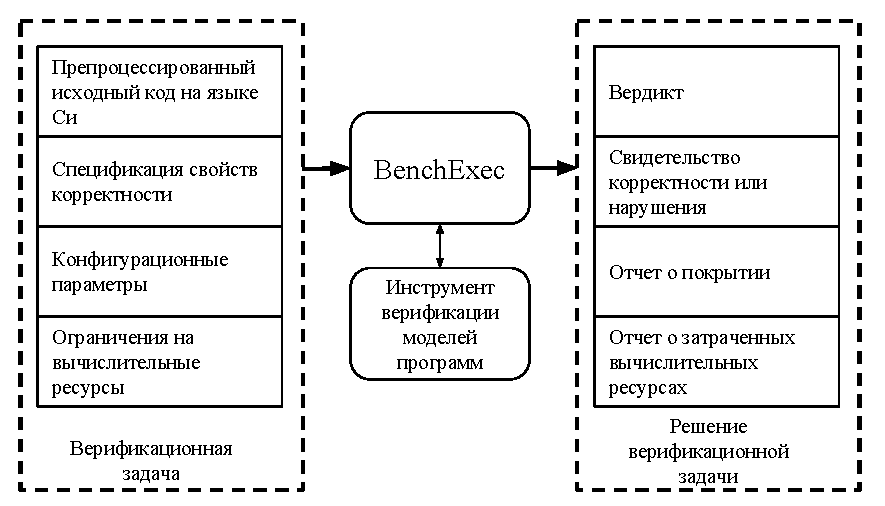
\includegraphics[scale=1]{BenchExec}
\caption{Схема решения верификационных задач.}
\label{figure:benchexec}
\end{figure}

Описание верификационной задачи представляет собой XML файл, который содержит пути к файлам с исходным кодом и спецификацией свойств корректности.
Верификационная задача может дополнительно содержать ограничения на вычислительные ресурсы и конфигурационные параметры для запуска конкретного инструмента верификации моделей программ, но формат не предусматривает единого способа задания конфигурационных параметров в едином виде для разных инструментов верификации.

Отчет о решении верификационной задачи содержит вердикт, пути к файлам свидетельств корректности или нарушения, отчет о покрытии и отчет о затраченных вычислительных ресурсах, включая время решения верификационной задачи, процессорное времени, максимальный объем используемой оперативной и дисковой памяти во время решения.

Вердикт --- это главный результат решения верификационной задачи, который может принимать значения \textbf{True}, \textbf{False} или \textbf{Unknown}.
Значение True означает, что выполнение свойств корректности доказано.
В этом случае инструмент выдает файл свидетельства корректности (англ. correctness witness).
Вердикт False соответствует обнаружению такого ошибочного пути выполнения программы (контрпримера), который опровергает тезис о выполнении свойства корректности.
Инструмент выдает ошибочный путь, содержащий предположения о значении переменных при выполнении инструкций программы, в виде файла свидетельства нарушения (англ. violation witness).
Если инструмент верификации моделей программ не смог доказать или опровергнуть выполнение свойств корректности при заданных ограничениях на вычислительные ресурсы, то вердикт принимает значение Unknown.

BenchExec использует механизм \textit{cgrpoups}~\cite{cgroups} ядра операционной системы Linux для ограничения и подсчета потребляемых процессорного времени и оперативной памяти, а для ограничения дисковой памяти и доступа к файловой системе используются возможности файловой системы \textit{Overlay}~cite{overlay}.
BenchExec останавливает выполнение инструмента при превышении им ограничения на доступные вычислительные ресурсы и в этом случае выдает вердикт Unknown.

Отчет о покрытии отражает ту часть кода, которая достижима из точки входа (функции \textit{main}).
При верификации небольших замкнутых программ, данный отчет обычно не несет большой практической пользы, так как инструменты верификации моделей программ анализируют все пути выполнения, возможные в программе.
Поэтому только некоторые инструменты верификации моделей программ в составе результатов решения верификационной задачи включают файл отчета о покрытии исходного кода программы~\cite{verificationcov}.
Но при верификации модулей программных систем, которые могут не являться замкнутыми программами и иметь несколько точек входа, данный отчет позволяет определить недостатки верификационной задачи, в частности неполноту модели окружения, которая рассмотрена в следующем разделе.

\subsection{Поддержка языка Си}
%Инструменты верификации моделей программ строят модель на основе исходного кода.
Для верификации программ на различных языках программирования инструменты используют специальное внутреннее представление.
Например, инструмент верификации моделей программ Corral опирается на инфраструктуру SMACK для трансляции программ во внутреннем представлении LLVM в программу на языке Boogie~\cite{tacas2015-hcelqr}.
А для работы с программами на языке программирования Си в инструменте CPAchecker~\cite{Beyer:2011:CTC} используется парсер Eclipse CDT.

Инструменты верификации моделей программ реализуют различные методы, но имеют схожие ограничения при верификации программ на языке Си:
\begin{itemize}
    \item фрагменты программы на языке ассемблера не поддерживаются большинством инструментов верификации моделей программ. Если программа содержит такие фрагменты, то либо инструменты игнорируют данный код (анализируют программу в предположении, что данный фрагмент на языке ассемблера не влияет на корректность программы), либо аварийно завершают свою работу.
    \item Инструменты, которые реализуют метод ограничиваемой проверки моделей~\cite{Biere03boundedmodel}, проверяют пути выполнения программы с фиксированным числом итераций и определенной глубиной рекурсии. Другие методы верификации моделей могут не иметь такого ограничения, например, метод k-индукции позволяет анализировать циклы любой длины~\cite{kinduction}.
    \item Инструменты верификации моделей программ имеют разные ограничения при верификации арифметики с указателями, битовыми операциями, операциями с плавающей точкой, строками, массивами, функциональными указателями, списками и т.д. Один инструмент, как правило, может иметь несколько реализаций способов построения модели программы и видов анализа для верификации программы с необходимым уровнем точности. 
    \item Инструменты верификации поддерживают небольшой набор моделей функций стандартной библиотеки языка Си и каждый инструмент имеет собственный список таких моделируемых функций.
    \item Проверку некоторых требований инструменты верификации моделей программ могут выполнять только для последовательных программ.
    Направление верификации параллельных программ развивается и широко представлены инструменты для проверки программ, использующих интерфейс управления потоками согласно стандарту POSIX.
\end{itemize}

\subsection{формализация требований при помощи свойств корректности}
Спецификация свойств корректности содержит формулы темпоральной логики.
Проверка каждого свойства корректности задается при помощи следующего выражения:

\[CHECK( init(main()), LTL(\phi) )\]

При верификации моделей программ анализируются все возможные пути выполнения, которые начинаются из функции \textit{точки входа}.
Имя такой функции указывается в качестве первого аргумента $CHECK$.
В данном примере точкой входа является функция \textit{main}.
Формула $\phi$ соответствует проверяемому свойству корректности и может принимать следующий вид:
\begin{itemize}
\item $\mathbf{G}~!call(\_\_VERIFIER\_error())$ --- свойство недостижимости ошибочного оператора (в данном примере вызова функции \textit{\_\_VERIFIER\_error});
\item $\mathbf{G}~!overflow$ --- свойство непереполнения целочисленного знакового типа;
\item $\mathbf{G}~valid-free$, $\mathbf{G}~valid-deref$, $\mathbf{G}~valid-memtrack$ --- свойство безопасного доступа к памяти, выраженное в виде совокупности трех формул.
\item $\mathbf{F}~end$ --- свойство завершимости.
\end{itemize}

На практике задачу проверки какого-либо требования к программе сводят к проверке одного или нескольких поддерживаемых свойств корректности.
Для этого разрабатывается модель требования на языке программирования Си для добавления к исходному коду верификационной задачи, в том числе и при помощи инструментации оригинального исходного кода верифицируемой программы.
При проверке таких требований, как, например, завершимость программы или корректность работы с памятью такая модель может быть тривиальной или не требоваться вовсе, если инструмент верификации поддерживает проверку соответствующего свойства корректности.
Для функциональных требований или программных контрактов, как правило, нужно разработать существенно более сложную модель требования для сведения задачи к доказательству выполнения свойства недостижимости ошибочного оператора.

Отдельные инструменты верификации моделей программ поддерживают другие способы формализации требований, основанные на спецификации требования при помощи некоторого языка предметной области или формализма.
Например, в инструменте верификации CPAchecker можно задать модель некоторых требований в виде автомата~\cite{Apel:2016}, но такой подход не позволяет применять другие инструменты верификации.

Инструменты верификации моделей программ выполняют анализ верификационной задачи до первого найденного нарушения свойства корректности.
Данная особенность обусловлена тем, что инструменты предназначены для доказательства корректности всей программы в составе верификационной задачи, а не отдельных функций или блоков кода.
Эксперименты по повторному использованию результатов верификации нескольких свойств корректности и требований ведутся разными командами исследователей~\cite{CPAreuse, CMBCreuse, Apel:2016}. 
На практике это затрудняет разработку моделей требований и может привести к ухудшению результатов, если какая-либо модель требования недостаточно точна и приводит к большому числу ложных срабатываний или требует слишком много вычислительных ресурсов для проверки.

В данной работе рассматривается проверка только таких требований, для любых нарушений которых может быть найден ошибочный путь (контрпример) конечной длины.
Из рассмотренных свойств корректности к таким не относится только свойство завершимости.

\subsection{Моделирование окружения}
Инструменты верификации моделей программ предназначены для верификации замкнутых программ на языке программирования Си.
Такие программы имеют одну точку входа, например, функцию \textit{main} и опираются только на стандартную библиотеку языка Си.

На практике программы и в особенности их отдельные модули взаимодействуют с окружением, в которое входят другие модули программы и операционная система.
Для верификации такого модуля программы требуется специфицировать предположения о взаимодействии модуля с окружением.
Для этого следует, как правило, разработать модель окружения на языке Си.
Такая модель содержит недостающие определения функций и реализует искусственную точку входа, если верифицируемый модуль программы не содержит функции \textit{main} и определяет несколько функций, вызываемых в окружении.
%Вызов точек входа в модели должен выполняться согласно устройству окружения программы.

Сообщество разработчиков SV"~COMP не предоставляет специальных средств для автоматизации или сокращения трудоемкости разработки моделей окружения.
Наиболее распространенный подход при моделировании --- это разработка модели окружения в виде отдельных фрагментов на языке программирования Си и инструментация исходного кода автоматически или вручную для добавления данных фрагментов в исходный код модуля.

Неточность и неполнота модели окружения может приводить и к пропуску ошибок, и к ложным предупреждениям об ошибках.
Исследователи подтверждают, что моделирование окружения на практике необходимо при верификации отдельных модулей программных систем и может требовать значительных усилий~\cite{subsystems:Trudy, ZakharovEnv2015, ModelingLargeSystems, neville2016a, FlashDriver, ConcurBugsRakamaric, Ivancic:2015:SSS}.
В то же время для поиска ошибок, а не для формальной верификации, сложность модели окружения может быть значительно снижена по сравнению с устройством реального окружения~\cite{ZakharovEnv2015}.

Некоторые неопределенные функции из стандартной библиотеки языка программирования Си поддерживаются инструментами верификации моделей программ и не требуют явного моделирования.
Для остальных неопределенных функций без разработанной вручную модели инструменты верификации предполагают возвращение неопределенного значения в соответствии с сигнатурой функции и отсутствие побочных эффектов, то есть выполнение функции без изменения значений аргументов, глобальных переменных и памяти во время выполнения.

При моделировании окружения программ на языке программирования Си используются специальные функции, поддерживаемые инструментами верификации, разрабатываемыми в рамках сообщества SV"~COMP.
Например, функция \textit{\_\_VERIFIER\_nondet\_int} возвращает неопределенное целое число, что упрощает моделирование неопределенного поведения окружения.
Полезной при моделировании окружения является функция \textit{\_\_VERIFIER\_assume}.
Единственным аргументом данной функции служит логическое выражение над переменными программы.
Пути, на которых выражение принимает ложное значение, не могут служить контрпримерами для выдачи предупреждений об ошибках.
Некоторые инструменты верификации моделей программ поддерживают более широкий набор функций для моделирования окружения.
Например, режим работы инструмента CPAchecker с анализом символических графов памяти (SMG) позволяет использовать функции \textit{external\_allocated\_data} для обозначения внешней <<корректной>> памяти, выделенной в модели окружения, и ошибки, связанные с некорректным доступом к такой памяти, игнорируются.

\subsection{Требования к вычислительным ресурсам}
При проверке программы с большим количеством циклов, ветвлений или потоков возникает проблема взрыва числа состояний в модели, построенной инструментом верификации для проверки требования на основе исходного кода данной программы.
О существовании метода оценки объема требуемых вычислительных ресурсов для успешного завершения верификации автору не известно.
Сколько потребуется вычислительных ресурсов зависит от многих факторов, например, от проверяемых свойств корректности, конфигурационных параметров инструмента, используемого SMT решателя, сложности исходного кода, производительности вычислительной системы.
Инструменты реализуют разные способы построения модели и алгоритмы для ее верификации.
Снижение точности модели или анализа не приводит к пропуску нарушений требований, но способно вызывать ложные сообщения об ошибках. 
Выбор наиболее точных подходов, как правило, всегда приводит к существенному увеличению времени работы инструментов верификации.

При сравнительном анализе инструментов верификации моделей программ в рамках SV"~COMP на решение каждой верификационной задачи отводится 15 минут процессорного времени и 15 GB оперативной памяти.
Данных ограничений бывает достаточно для верификации программ размером несколько десятков тысяч строк кода на языке программирования Си.

\subsection{Оценка результатов верификации}
Для проверки корректности вердикта сообществом SV"~COMP предложен подход валидации свидетельств корректности и нарушений при помощи специальных инструментов верификации моделей программ --- \textit{валидаторов}~\cite{Beyer:2015:WVS,Beyer:2016:CWE}.
Для выявления ложных сообщений об ошибках свидетельства нарушений могут быть валидированы и при помощи генерации тестов для проверки выполнимости ошибочного пути динамически~\cite{Beyer2018TestsFW, Beyer:2004:GTC}.

При верификации модуля программы верификационная задача содержит модель требования и модель окружения.
Упомянутые методы валидации позволяют определить неверный вердикт, причиной которого может быть только неточный анализ инструмента верификации моделей программ.
Если некорректный вердикт получен из-за неточной или неполной модели окружения или требования, то необходимо выполнение экспертизы свидетельств пользователем.

Свидетельства корректности и нарушения предназначены для валидаторов, которые в составе входных данных получают исходный код верификационной задачи.
Поэтому инструменты опускают важные фрагменты ошибочных путей при выдаче свидетельств нарушения, а для свидетельств корректности предоставляют только инварианты циклов программы.
Следовательно, даже с использованием средств визуализации, без вспомогательной информации анализ свидетельств вручную является трудным.

BenchExec предоставляет средство визуализации свидетельств нарушений, которое, однако, имеет ряд недостатков:
\begin{itemize}
    \item низкая масштабируемость и визуализация только простых ошибочных путей длиной несколько сотен строк кода;
    \item невозможность отличить код моделей окружения и требований от оригинального исходного кода верифицируемой программы;
    \item отсутствие связи между препроцессированным исходным кодом верификационной задачи и исходным кодом программы до препроцессирования;
    \item отсутствие подсказок и сообщений для пользователя о причине и вероятном месте ошибки в программе.
\end{itemize}

\section{Ограничения подходов к применению инструментов верификации моделей Си-программ}
% Применение инструментов на практике CBMC
Инструменты верификации моделей программ применяются для проверки требований различных программных систем на языке программирования Си:
\begin{itemize}
    \item При помощи CMBC была проверена реализация алгоритма сжатия\break Brotli\cite{brotli} и показана возможность обнаружения известной уязвимости~\cite{neville2016a}.
    \item Инструмент CMBC используется для генерации тестов в рамках системы BTC EMBEDDEDTESTER для тестирования встраиваемого программного обеспечения~\cite{CMBCreuse}. CBMC применялся для верификации операционной системы TinyOS и другого программного обеспечения для встраиваемых систем~\cite{Schlich2009, Bucur:2010:SVT}. Также инструменты СBMC и CPAchecker были интегрированы в среду для разработки встраиваемого программного обеспечения $mbeddr$~\cite{mbeddr}. 
    \item Ряд работ рассматривает верификацию драйверов~\cite{Post:2009:TAS,Witkowski:2007:MCC, ModelingLargeSystems, FlashDriver, ConcurBugsRakamaric} и файловых систем~\cite{Galloway:2008:MLV, Yang:2006:UMC}.
    \item При помощи CMC была выполнена проверка реализации сетевого протокола TCP в ядре операционной системы Linux~\cite{Musuvathi:2004:MCL}.
    \item Известны примеры верификации моделей программ на языке Си++. Например, ESBMC++ предлагается использовать для проверки приложений на основе фреймворка Qt~\cite{QTverification}.
\end{itemize}

Перечисленные работы нацелены на поиск ошибок, а не на доказательство корректности модулей Си-программ.
Полученные результаты подтверждают возможность обнаружения ошибок в крупных программных системах на языке программирования Си.
В то же время, работы выполнялись разработчиками инструментов верификации или исследователями с хорошей математической подготовкой.
В процессе верификации требуется модифицировать исходный код, моделировать окружение и требования, изучать ложные срабатывания, устранять их причины.
В большинстве работ весь процесс верификации детально не описан и трудозатраты не представлены.
В некоторых случаях отдельные шаги процесса верификации были автоматизированы, но авторы не предложили каких-либо средств, применимых при верификации другого программного обеспечения.

Основную сложность при подготовке программ к верификации составляют шаги моделирования окружения и формализации требований.
Модели окружения в перечисленных работах разрабатываются на языке Си.
Например, некоторые авторы признают, что только для разработки модели окружения отдельного драйвера операционной системы вручную может требоваться около одного человеко-месяца~\cite{ConcurBugsRakamaric}.
Еще одним ограничением подхода разработки моделей вручную на языке Си является возможность проверять только определенный тип требований.
Например, если модель окружения разработана для применения инструмента верификации моделей программ для проверки требований, сведенных к доказательству недостижимости ошибочного оператора в последовательной программе, то для поиска гонок по данным придется разрабатывать новую параллельную модель окружения.
Схожие ограничения имеет подход, предложенный для поиска ошибок в драйверах при помощи символьного выполнения и реализованный в инструменте SymDrive~\cite{Renzelmann:2012:STD}.
Для применения инструмента также требуется разработать вручную модель окружения на языке программирования Си, которая применима только при поиске ошибок определенного вида.

Для описания моделей различных систем применяется множество языков и формализмов~\cite{Seshia2018}.
Но для применения инструментов верификации моделей Си-программ верификационная задача должна включать исходный код именно на языке программирования Си.
По этой причине на практике не используются подходы к моделированию окружения, которые предполагают описание модели окружения на языке, значительно отличающемся от языка Си по синтаксису или семантике.

Еще одним направлением применения метода проверки моделей для проверки программного обеспечения является композиционная верификация программ на языках Си\IntroCite{LTSA} и Java\IntroCite{Giannakopoulou:2004:AVS, Parizek:2007:SGE, Zhai:2016:AMG,parizek2007partial,Tkachuk:2003:AEG} на основе спецификаций предположений об окружении.
Отличительной особенностью данных работ является цель доказать корректность целевого модуля или программы формально.
Трудоемкость композиционной верификации велика и доказательства корректности могут быть получены только для небольших программ или модулей.
Для описания моделей окружения используется либо непосредственно язык программирования, на котором разработана программа, либо некоторые языки предметной области, которые позволяют описать ограничения на последовательность вызова точек входа модуля в виде спецификации.
Предложенные методы синтеза моделей окружения на основе таких спецификаций позволяют снизить трудоемкость подготовки моделей окружения для классов на языке Java, но не учитывают особенностей устройства интерфейса программ на языке Си.

Для автоматизированного применения инструментов верификации моделей Си-программ для проверки требований к модулям крупных программных систем требуется автоматизировать синтез верификационных задач.
В этом случае возникает задача декомпозиции программы на модули, состоящие из наборов файлов с исходным кодом на языке программирования Си.
Схожие формулировки задачи декомпозиции программы встречаются и в других предметных областях, например, в работах, посвященных рефакторингу.
Отличительной особенностью задачи декомпозиции в области верификации моделей программ является трудность формализации критериев, которым должны удовлетворять полученные после декомпозиции модули программы.
Автору неизвестно о работах, которые предложили бы метод проверки с достаточным уровнем точности возможности успешного решения верификационной задачи, полученной на основе некоторого модуля программы.
Как было ранее упомянуто при рассмотрении вопроса масштабируемости инструментов верификации, процесс верификации зависит от множества факторов.
Схожая трудность возникает при попытке оценить трудоемкость разработки моделей окружения для заданного модуля.
Число точек входа и неопределенных функций в модуле лишь косвенно влияет на трудоемкость разработки таких моделей.
Поэтому задача декомпозиции для каждой верифицируемой программной системы решается с учетом устройства ее модулей и о попытках обобщить полученные результаты для декомпозиции программ, имеющих разный вид и устройство, автору не известно.

Для автоматизированного применения инструментов верификации моделей программ были реализованы системы верификации.
Системы верификации LDV Tools~\cite{Zakharov2015} и SDV~\cite{Ball2004} нацелены на проверку требований корректного использования интерфейса ядра операционной системы (ОС) в драйверах Linux и Windows соответственно.
Система верификации DC2~\cite{Ivancic:2015:SSS} позволяет проверять требование корректности работы с памятью к программному обеспечению встраиваемых систем.

% Система статической верификации драйеров Windows
Система верификации SDV была включена в состав набора средств для разработки драйверов Microsoft Windows Driver Development Kit в 2006 году.
SDV может быть использована в качестве плагина среды разработки Visual Studio.
Исходный код системы верификации является закрытым.

% Подготовка драйвера и Модель окружения
Система поддерживает верификацию драйверов устройств ОС Windows определенных типов.
Для таких типов были разработаны модели окружения на языке программирования Си вручную.
Модели позволяют проверять исходный код драйверов обработки IRP запросов и драйверов минипорта для сетевых устройств отдельно от исходного кода ОС Windows.
Обработчики проверяемого драйвера, которые являются его точками входа, должны быть аннотированы пользователем вручную.

В состав системы верификации входит несколько сотен спецификаций требований.
Для их задания используется аспектно-ориентированное расширение языка программирования Си SLIC (англ. Specification Language for Interface Checking)~\cite{SLIC}.
Язык схож с языком Си по синтаксису, поэтому в разработке спецификаций корректности использования интерфейса ядра драйвером участвуют не только эксперты в области верификации.

% Инструмент верификации
Первоначально в системе применялся инструмент верификации моделей программ SLAM~\cite{Ball:2011:DSM}.
Затем стало возможным использование инструментов SLAM2~\cite{SLAM2}, Yogi~\cite{Yogi} и Q, основанном на CORRAL~\cite{Lal:2014:PSD}. 
Перечисленные инструменты не поддерживают предложенные в SV"~COMP форматы верификационных задач.

% Вывод
Система верификации SDV имеет высокую практическую значимость:
\begin{itemize}
\item Система верификации используется не только специалистами в области верификации, но и разработчиками драйверов ОС Windows.
\item Результаты верификации имеют крайне низкий процент ложных сообщений об ошибках. 
В работе о SLAM2 сообщается, что этот показатель составляет 4\%~\cite{SLAM2}.
\item По состоянию на 2010 год при помощи системы верификации было выявлено 270 ошибок, что существенно повысило надежность драйверов операционной системы Windows, согласно утверждениям разработчиков системы верификации.
\end{itemize}

% Система статической верификации драйверов Linux LDV Tools
В рамках проекта LDV (англ. Linux Drivers Verification) по верификации драйверов ядра ОС Linux, который начался в 2012 году, была разработана система верификации LDV Tools~\cite{configurable:Trudy, Zakharov2015, Beyer:2012:LDV}.

Система верификации выполняет синтез моделей окружения и моделей требований.
Для синтеза моделей окружения используется подход вызова обработчиков драйверов на основе шаблонов.
При помощи шаблонов могут быть заданы ограничения на порядок вызова обработчиков, но описать ограничения на параметры при вызове реализованный подход не позволяет.
Процесс подготовки моделей окружения не предполагает возможности проверки разных свойств корректности, отличных от свойства недостижимости ошибочного оператора.

Система статической верификации позволяет проверять несколько десятков специальных требований корректности использования интерфейса ядра в драйверах, например, корректность синхронизации процессов, инициализации, захвата и освобождения различных ресурсов, передачи параметров функциям ядра в зависимости от контекста выполнения.
Каждое требование формализовано в виде контрактной спецификации на аспектном расширении языка Си.
Для синтеза верификационных задач исходный код драйвера инструментируется при помощи инструмента CIF для добавления моделей окружения и требований к исходному коду драйверов~\cite{Novikov2013}.

Система верификации позволяет использовать инструменты верификации моделей программ CBMC, CPAchecker и Blast, разрабатываемые и поддерживаемые сообществом SV"~COMP.
Но инструмент BenchExec в системе не используется, поэтому для применения инструментов разработаны адаптеры для конвертирования входных и выходных данных в необходимые форматы.

Одним из главных недостатков системы является низкая масштабируемость.
Система верификации не позволяет синтезировать верификационные задачи параллельно, что значительно увеличивает время получения результатов.
Например, для верификации всех модулей ядра Linux, которых в исходном коде ядра порядка четырех тысяч, на соответствие одному требованию требуется более суток.
Архитектура системы верификации имеет ряд важных ограничений, например, систему не может использовать несколько пользователей одновременно, что при высоких требованиях к вычислительным ресурсам затрудняет ее использование в рамках распределенных вычислительных систем.

Система верификации позволила найти более 200 ошибок в драйверах ОС Linux, которые были подтверждены их разработчиками.
В то же время число ложных предупреждений об ошибках в результатах верификации достаточно велико.
Согласно результатам, представленным в работах~\cite{configurable:Trudy, Zakharov2015}, 60\% ложных сообщений об ошибках вызваны именно неточностью моделей окружения, для исправления которых в системе не предусмотрено необходимых средств.

% Система верификации DC2
Система верификации DC2 нацелена на проверку требований корректности работы с памятью к программному обеспечению встраиваемых систем ~\cite{Ivancic:2015:SSS}.
Система является закрытым проектом, разрабатываемым компанией NEC.

% Модель окружения
Система верификации реализует метод уточнения модели окружения по контр-примеру CEGER (англ. Counter-Example Guided Environment Refinement).
Перед верификацией система выполняет легковесный межпроцедурный статический анализ исходного кода программы \textsc{SpecTackle}.
Анализ нацелен на генерацию моделей окружения с условиями (англ. constraints) для разных точек программы, например, предусловий или постусловий вызова функций.
Анализ выделяет условия, связанные с разыменованием указателей, выделением памяти, обращениями к массивам.
Модель окружения генерируются в виде аннотаций к исходному коду.
\textsc{SpecTackle} опирается на различные эвристики и может генерировать некорректные модели окружения.
Предполагается, что пользователь может исправить модели окружения вручную, выполняя процесс верификации итеративно.
Данный подход автоматизирует подготовку модели окружения для программ размера несколько сотен тысяч строк кода на языке Си.
Предложенный метод нацелен на замену функций на их упрощенные заглушки, но не позволяет генерировать вызовы точек входа.
Данным недостатком обладают и методы верификации программ с ограничением области видимости (англ. scope-bounded verification) и межпроцедурного статического анализа.

В качестве единственного инструмента верификации используется VARVEL, разрабатываемый корпорацией NEC.
Инструмент в системе верификации используется для проверки свойства корректности работы с памятью и позволяет обнаруживать такие дефекты, как, например, выход за границу массива, повторное освобождение памяти, утечки памяти.

% Анализ результатов
Сообщается об успешном пилотном применении системы верификации разработчиками компании для проверки проектов размера более сотни тысяч строк кода.
В рамках применения системы верификации удалось обнаружить и исправить более десятка ошибок. 
Так как проект является закрытым, то оценить в полной мере применимость предложенных методов для верификации различных программ на языке программирования Си не удается.

\begin{table}
\centering
\begin{tabular}{ | l | c | c | c | }
\hline
Критерий сравнения & SDV & LDV & DC2 \\
\hline
\begin{tabular}{@{}l@{}} Поддержка адаптивной декомпозиции программ\end{tabular} & \ding{55} & \ding{55} & \ding{55} \\
\hline
\begin{tabular}{@{}l@{}} Наличие средств для разработки или \\ исправления моделей окружения  \end{tabular} & \ding{51} & \ding{55} & \ding{55} \\
\hline
\begin{tabular}{@{}l@{}} Синтез моделей окружения\end{tabular} & \ding{55} & \ding{51} & \ding{51} \\
\hline
\begin{tabular}{@{}l@{}} Наличие средств для разработки или \\ исправления моделей требований \end{tabular} & \ding{51} & \ding{51} & \ding{55} \\
\hline
\begin{tabular}{@{}l@{}} Синтез моделей требований \end{tabular} & \ding{51} & \ding{51} & \ding{51} \\
\hline
\begin{tabular}{@{}l@{}} Поддержка проверки разных свойств корректности\end{tabular} & \ding{55} & \ding{55} & \ding{55} \\
\hline
\end{tabular}
\caption{Сравнение систем верификации моделей программ.}
\label{table:systems}
\end{table}

В таблице~\ref{table:systems} представлено сравнение систем верификации моделей программ.
Рассмотренные системы верификации не предлагают средств автоматизации декомпозиции программ разных видов.
Средства для разработки моделей окружения, в которых можно задать и вызов точек входа, и модели отсутствующих функций, реализованы только в SDV, но разработка моделей окружения предусмотрена только на языке Си.
Системы верификации нацелены на проверку конкретных видов требований к определенным программным системам и не предполагают возможности адаптировать процесс синтеза верификационных задач для верификации других программных систем.
Системы верификации LDV и SDV позволяют проверять выполнение только свойства недостижимости ошибочного оператора, а DC2 только свойства корректности работы с памятью.
LDV, и SDV реализуют подходы для сведения проверки различных требований к проверке свойства недостижимости ошибочного оператора.

Согласно рассмотренным работам, при применении инструментов верификации моделей Си-программ для проверки требований к крупным программным системам основными ограничениями остаются отсутствие методов автоматизации декомпозиции программ разных видов и высокая трудоемкость моделирования окружения.
Существующие системы верификации, предназначенные для автоматизации применения инструментов верификации, не предусматривают адаптации процесса синтеза верификационных задач для различных программных систем и для проверки требований к ним, формализованных на основе различных свойств корректности.

\section{Методы распараллеливания верификации моделей программ}

Инструменты верификации моделей программ реализуют, как правило, последовательные алгоритмы верификации моделей.
Они не используют преимуществ многоядерных и графических процессоров или распределенных вычислительных систем.
Применение инструментов верификации для проверки требований к крупным программным системам на языке Си может требовать решения большого числа верификационных задач, что подтверждается опытом практического применения систем верификации LDV и SDV.
Поэтому следует рассмотреть методы сокращения времени решения совокупности верификационных задач и каждой задачи в отдельности.
За последние годы появилось много примеров применения высокопроизводительных вычислений (англ. high-perfromance computing) в области верификации моделей~\cite{survey:new}.
Чтобы определить на какие вычислительные системы впоследствии могут быть рассчитаны инструменты верификации моделей программ, требуется рассмотреть исследования в данной области. 

% Кластеры
\subsection{Распределенные вычислительные системы}
Распределенные вычислительные системы (вычислительные кластеры) широко используются для повышения производительности различных приложений.
Параллельные версии алгоритмов для верификации моделей с применением вычислительных кластеров были предложены до появления инструментов верификации моделей программ.
Например, параллельная реализация инструмента верификации моделей Mur$\varphi$ была представлена уже в 1997 году~\cite{Stern97parallelizingthe}.
Алгоритм, представленный в работе, предполагает распределение частей пространства состояний проверяемой модели для обработки между узлам вычислительного кластера при помощи хэш-функции.
Другим примером применения распределенных вычислительных систем является работа, опубликованная в 1999 году разработчиками инструмента SPIN~\cite{Lerda1999}.
Инструмент DiVinE реализует результаты современного исследования в данной области~\cite{VW86b}.
Авторы представили версии алгоритмов как для распределенных вычислительных систем, так и для многоядерных процессоров с общей памятью ~\cite{Barnat:2010:SSM,HiBi.2009,Barnat2009,Barnat5161000}.
Наилучшее ускорение составило 8 раз относительно последовательной версии инструмента при использовании 10 узлов распределенной вычислительной системы.

Многие инструменты верификации моделей программ реализуют алгоритм уточнения абстракции по контрпримеру~\cite{Clarke:2003:CAR}.
Параллельная версия данного алгоритма для верификации моделей реализована в инструменте ARMC~\cite{Lopes2011}.
Алгоритм, представленный в работе, подразумевает использование одного главного и нескольких рабочих узлов.
Главный узел выполняет интерполяцию, проверку выполнимости формулы пути и хранит граф пространства состояний модели программы.
Рабочие узлы выполняют обход подмножества пространства состояний, полученного от главного узла, и отправляют результат работы на главный узел после расчета новых состояний.
Авторы уделили внимание проблеме воспроизведения результатов.
Наибольшее ускорение составило 28 раз относительно последовательной версии алгоритма при использовании вычислительного кластера из 40 узлов.

Облачные сервисы представляют собой масштабируемую распределенную систему, число задействованных узлов в которой может изменяться в зависимости от сложности решаемой задачи.
Универсальными облачными являются сервисы IaaS (англ. infrastructure as a service) и PaaS (platform as a service).
Сервисы IaaS позволяют получить распределенную вычислительную систему, состоящую из виртуальных машин с заданными характеристиками в качестве вычислительных узлов.
Примером такого сервиса является Amazon Elastic Cloud EC2~\cite{ec2}.
Альтернативным решением являются PaaS облачные сервисы, которые предоставляют пользователю возможность запускать экземпляры целевого приложения, обрабатывающие независимые запросы, в специальной вычислительной среде.
Сервис динамически регулирует число активных экземпляров приложения в зависимости от числа ожидающих обработки запросов.
Примером такой системы является Google App Engine~\cite{gae}.

% А также верификацию в PAAS GAE
Инструмент верификации моделей программ CPAchecker был адаптирован для запуска в облачном сервисе Google App Engine~\cite{Beyer:2014:SVG}. 
Для этого потребовалось отказаться от запуска вспомогательных сторонних компонентов в рамках работы инструмента, а также использовать заданный интерфейс для доступа к ресурсам операционной системы, например, к дисковой памяти.
Основным недостатком использования данного облачного сервиса на практике является запрет на задание достаточно высоких ограничений на вычислительные ресурсы, из-за чего верифицировать модули программ размером десятки тысяч строк кода на языке Си не удается.

Существуют также и специальные облачные сервисы, нацеленные на решение конкретной задачи в заданной предметной области.
Проект VerifierCloud~\cite{VerifierCloud} представляет собой облачный сервис, который также управляет вычислительным кластером для запуска инструментов верификации моделей программ изолированно на разных вычислительных узлах.
Данный проект широко используется для выполнения сравнительного анализа инструментов верификации моделей программ сообществом SV"~COMP~\cite{SVCOMP2014,Beyer2016}.
Разработчики также предоставляют специальный облачный сервис для решения верификационных задач при помощи инструмента CPAchecker.

% Многоядерные системы 
\subsection{Многоядерные вычислительные системы}
Современные процессоры имеют несколько ядер c функцией одновременной многопоточности (англ. simultaneous multithreading — SMT).
Для того, чтобы полноценно использовать многоядерную архитектуру необходимо реализовать параллельные алгоритмы, эффективно использующие разделяемую память.

Разработчики инструментов верификации моделей представили ряд работ по применению параллельных алгоритмов для работы с разделяемой памятью. 
Алгоритмы реализованы в таких инструментах, как SPIN~\cite{Holzmann:2003:SMC,5661793,Holzmann:2012:PSM}, DiVinE~\cite{Brim2001,BARNAT2003,Brim2004,Brim:2006:OVD,Barnat:2010:SSM} и LTSmin~\cite{Laarman2011,Laarman:2010:BMR}.
В представленных работах авторы уделили внимание проблеме реализации структур данных для хранения пространства состояний и параллельного доступа к ним из разных потоков.
При использовании многопоточных процессоров нехватка памяти при верификации снова выходит на первый план.
Для преодоления данной проблемы в SPIN было реализовано сокращение частичных порядков~\cite{Bosnacki2006}, а разработчики LTSmin предложили алгоритм Collapse для сжатия данных~\cite{Laarman2011mem}.

В рассмотренных работах были достигнуты различные результаты.
Но в все инструменты смогли достигнуть ускорения порядка 5-10 раз при эффективности (отношение ускорения к числу потоков) 50\% при использовании до 10-30 потоков.

\subsubsection{Графические процессоры}
Успехи в разработке высокопроизводительных графических процессоров привели к широкому их распространению для организации вычислений в различных сферах.
А появление такой платформы как NVIDIA CUDA сделало применение графических процессоров менее трудоемким~\cite{cuda}.
Автору не известны применения графических процессоров для верификации моделей программ, но результаты экспериментов по верификации моделей при помощи данной аппаратуры уже опубликованы разными командами исследователей.

Современные графические процессоры обладают высокой производительностью, но имеют свои отличительные особенности.
Графические процессоры адаптированы под операции с данными в матрично-векторной форме.
Исходный код отличается от кода для центрального процессора.
Из-за более длительного такта системные вызовы и ожидания при выполнении существенно снижают производительность.
Кроме того, графические процессоры обладают своей иерархией памяти и объем соответствующей разделяемой памяти обычно значительно меньше, чем объем оперативной памяти.

Разработчики инструмента DiVinE представили ряд работ, посвященных применению графических процессоров при проверке моделей~\cite{Barnat2009CUDA,Barnat2010CUDA,Barnat2012CUDA}.
Авторы адаптировали алгоритм MAP к матрично-векторной форме, а также реализовали параллельное выполнение центральным процессором поиска допускающего цикла.
В работе сообщается об ускорении в среднем в пять раз относительно последовательной версии инструмента, использующей только центральный процессор.
В работе, посвященной вероятностной верификации моделей (англ. probabilistic model checking), предлагается использовать обратную польскую запись~\cite{Burks:1954:ALM} для описания изменения состояний в модели~\cite{Bosnacki2009}.
Реализация алгоритма с использованием NVIDIA CUDA в инструменте SPIN представлена в работе~\cite{Bartocci:2014:TGS}.
Авторы сообщают также об ускорении до 7 раз по сравнению с последовательной версией алгоритма для центрального процессора.
Еще одним примером вероятностной проверки моделей является реализация инструмента PRISM~\cite{Kwiatkowska2002,Bosnacki:2010:GEP}.
Ряд работ опубликовали разработчики инструмента GPUexplore, нацеленного на верификацию моделей с явными значениями (англ. explicit state model checking)~\cite{Wijs2014,Wijs2016GPUexplore2U,Wijs2014,Neele2016}.
Авторы заявляют об ускорении верификации вплоть до 100 раз.

Результаты представленных выше работ демонстрируют возможность существенно сократить время верификации моделей с использованием графических процессоров.
В то же время верификация моделей с большим числом состояний при помощи графических процессоров затруднительна из-за ограниченного объема доступной памяти, и это ставит под сомнение эффективность данного направления для верификации моделей программ.
Чтобы достичь высокой производительности необходимо оптимизировать представление данных, что требует от разработчика хорошего понимания устройства иерархии памяти в графических процессорах, которая также развивается с появлением новых версий аппаратуры.

\subsection{Выводы}
Для сокращения времени решения верификационных задач при автоматизированном применении инструментов верификации моделей программ для проверки требований к крупным программным системам на языке программирования Си в данной работе предпочтение отдается методам распределенного параллельного решения верификационных задач с использованием вычислительных кластеров, IaaS платформ и специальных облачных сервисов.
Данный подход позволит применять как доступные сегодня инструменты верификации моделей программ, которые реализуют последовательные алгоритмы, так и инструменты, реализующие алгоритмы для многоядерных процессоров, эффективность которых показана в упомянутых работах по верификации моделей.

% Промежуточный вывод касательно верификационных задач SV"~COMP
\section{Требования к системе верификации моделей крупных программных систем на языке Си}
Данная работа посвящена развитию систем верификации моделей Си-программ для преодоления существующих ограничений, возникающих при их применении к крупным программным системам.
Для преодоления данных ограничений необходимо в первую очередь сократить трудоемкость подготовки верификационных задач и время их решения.
Для этого предлагается разработать новые методы автоматизированных декомпозиции Си-программ и синтеза моделей окружения, удовлетворяющие следующим требованиям:
\begin{itemize}
    \item Декомпозицию и синтез моделей окружения следует  автоматизировать таким образом, чтобы пользователь имел возможность выполнять адаптацию данных процессов, выполняемых при генерации верификационных задач, для разных программ и при проверке различных видов требований, предъявляемых к этим программам.
    Адаптацию предлагается выполнять при помощи конфигурирования и разработки спецификаций.
    \item Синтез моделей окружения следует выполнять на основе подготовленных вручную спецификаций предположений об окружении.
    Формат спецификаций должен позволять описывать и модели вызова точек входа модулей программ, и модели неопределенных функций.
    \item Для применения различных инструментов верификации моделей Си-программ следует использовать формат верификационных задач, разработанный сообществом SV"~COMP.
\end{itemize}

Предложенные методы предлагается реализовать в новой системе верификации, которая должна отвечать современным требованиям к системам такого класса.
В частности система должна обеспечивать следующие возможности:
\begin{itemize}
    \item Система верификации должна автоматизировать весь процесс верификации Си-программ, который включает этапы генерации верификационных задач, решения верификационных задач при помощи инструментов верификации и анализ результатов.
    \item Генерация и решение верификационных задач должны выполняться параллельно с использованием многоядерных процессоров для сокращения времени решения верификационных задач.
    \item Необходимо предусмотреть возможность применения распределенных вычислительных систем для параллельного решения верификационных задач.
    \item Требуется обеспечить воспроизводимость результатов верификации. 
    \item Система верификации должна предусматривать возможность одновременного использования несколькими пользователями. 
\end{itemize}

% Глава 2 Синтез верификационных задач
\chapter{Подготовка верификационных задач}

В данной главе описан процесс подготовки верификационных задач, в основе которого лежат новые методы автоматизированной декомпозиции Си-программ на модули и синтеза для них моделей окружения.

\section{Программный интерфейс модулей Си-программ}
Процесс генерации верификационных задач предполагает выполнение декомпозиции программной системы на языке программирования Си на модули, для каждого из которых в зависимости от его программного интерфейса выполняется подготовка соответствующих моделей окружения и требований.
Прежде чем изложить новые методы, рассмотрим что из себя представляет программный интерфейс таких модулей.

Модулем программы называется один или несколько Си-файлов с исходным кодом программы.
Построенная на основе модуля программы верификационная задача содержит препроцессированный исходный код данных файлов.
Исходный код верификационной задачи анализируется инструментом верификации моделей программ  отдельно от остальной программы и других верификационных задач.

Окружением модуля программы будем называть некоторый внешний по отношению к модулю исходный код, который содержит недостающие определения функций и который может обращаться к программному интерфейсу модуля, изменяя значения глобальных переменных и памяти, а также вызывая функции из модуля программы.
Некоторой частью окружения служит конкретный исходный код программы и заголовочных файлов системных библиотек, но некоторая часть окружения не может быть однозначно сопоставлена с каким-либо определенным исходным кодом на языке программирования Си.
Так, например, системные вызовы в исходном коде модуля зависят от реализации операционной системы, которая может быть разработана и не на языке программирования Си.

Программным интерфейсом модуля будем называть следующие глобальные переменные, функции, типы и макросы:
\begin{itemize}
    \item Функции относятся к программному интерфейсу, если они не определены в исходном коде модуля, но вызываются в нем. Определенные в исходном коде модуля функции, которые вызываются в окружении, будем называть \textit{точками входа}.
    Точки входа тоже являются частью программного интерфейса модуля.
    \item Аналогично макросы относятся к программному интерфейсу, если соответствующие макроподстановки используются и в окружении, и в исходном коде модуля.
    \item Параметры макрофункций и функций программного интерфейса тоже являются частью программного интерфейса модуля.
    \item Тип относится к программному интерфейсу, если он используется и в исходном коде модуля, и в окружении.
    Стандартные типы языка Си не относятся к программному интерфейсу модуля.
    \item К программному интерфейсу модуля относятся глобальные переменные, доступ к которым осуществляется и в исходном коде модуля, и в окружении.
\end{itemize}

Программный интерфейс нескольких модулей может содержать одни и те же элементы.
Так, например, программный интерфейс нескольких модулей программы может быть частично определен в заголовочных файлах, которые содержат декларации и определения функций и типов, декларации и инициализации глобальных переменных, а также макросы программного интерфейса модулей.

Рассмотрим пример модуля программы и его программный интерфейс:
\begin{lstlisting}[language=C,basicstyle=\small]
extern int b;
extern int f4(int a, int b);
int f1(int a, int b);
int f2(int a, int b);
static int f3(int a, int b)

int f1(int a) {
    return f3;
}

int f2(int a) {
    int c;
    
    c = nondet_int();
    return f4(a, c);
}

static int f3(int a) {
    if (a < b)
        return a - b;
    else
        return b - a;
}
\end{lstlisting}

Функции \textit{f1}, \textit{f2}, \textit{f4}, \textit{nondet\_int}, параметры функций и переменная \textit{b} определяют программный интерфейс данного модуля. 
Функции \textit{f1} и \textit{f2} являются точками входа, так как могут быть вызваны в окружении.
Функция \textit{f4} определена и переменная \textit{b} инициализирована в окружении, так как определение \textit{f4} и инициализация \textit{b} отсутствуют в примере.

Назовем \textit{событиями взаимодействия} модуля и окружения следующие операции на языке программирования Си:
\begin{itemize}
    \item Вызовы функций и макрофункций программного интерфейса модуля.
    \item Обращения на чтение или запись к глобальным переменным программного интерфейса модуля и к областям памяти в куче или на стеке, с указателями на которые выполняются операции и в исходном коде модуля, и в окружении.
\end{itemize}

\textit{Сценариями взаимодействия} модуля и окружения называются последовательности событий взаимодействия модуля и окружения, которые могут происходить при реальном выполнении программы, содержащей рассматриваемый модуль.
Сценарии взаимодействия, как правило, допускают разные пути выполнения программы с различными последовательностями событий взаимодействия в каждом из них.
К последовательностям событий в рамках сценария взаимодействия можно сформулировать следующие виды требований:
\begin{itemize}
    \item Ограничения на порядок следования событий взаимодействия, которые определяются:
        \begin{itemize}
            \item Отношениями до или после. Например, вызов одной функции происходит строго после другой. 
            \item Отношениями по возможности параллельного выполнения событий взаимодействия. Например, некоторые события выполняются параллельно или строго в одном и том же потоке или процессе программы.
            \item Отношениями зависимости событий, то есть события могут возникать обязательно или взаимоисключающим образом относительно друг друга. Например, вызов некоторой точки входа модуля программы выполняется строго при условии захвата определенного мютекса или другого механизма синхронизации.
        \end{itemize}
    \item События взаимодействия зависят по данным:
        \begin{itemize}
            \item В качестве параметров функций должны передаваться одни и те же значения или указатели на одну и ту же память. При выполнении доступа на чтение или запись должны быть прочитаны или записаны определенные данные.
            \item Могут быть справедливы ограничения на значения параметров функций и содержание определенных областей памяти. 
            Примером такого ограничения является требование, что некоторая точка входа модуля программы может быть вызвана с произвольным целым неотрицательным параметром.
        \end{itemize}
\end{itemize}

\textit{Моделью окружения} называется вспомогательный исходный код на языке программирования Си, который реализует сценарии взаимодействия модуля и окружения.
Такой код может состоять из отдельного файла, набора файлов или может быть представлен в виде отдельных фрагментов кода, предназначенных для вставки в исходный код модуля программы при помощи инструментации.
Любое описание модели окружения или ее модулей на каком-либо языке предметной области будем называть спецификацией модели окружения.

\textit{Полная} модель окружения реализует все возможные сценарии взаимодействия модуля программы и окружения, а \textit{корректная} модель окружения не реализует таких сценариев взаимодействия, которые не могут происходить при реальном выполнении программы.
В ряде случаев реализовать полную и корректную модель окружения бывает крайне трудно.
При поиске ошибок необходимо стремиться к полноте модели окружения, чтобы избежать пропуска ошибок.
Некорректная модель окружения может приводить к ложным предупреждениям об ошибках, но если их число невелико, то такая некорректная модель может быть применима на практике.
Надлежащий уровень полноты и корректности модели окружения может быть сложно оценить, а на практике он зависит в существенной степени от проверяемых требований.

Для преобразующих программ, у которых точкой входа является main, моделирование окружения сводится к разработке моделей функций, которые вызываются в исходном коде модуля и определены окружением.
Модель окружения для модулей библиотек и событийно-ориентированных программ имеет, как правило, более сложное устройство.
Для иллюстрации процесса моделирования окружения таких модулей рассмотрим следующий пример:
\begin{lstlisting}[language=C,basicstyle=\small]
/* drivers/tty/tty_io.c */
LIST_HEAD(tty_drivers);
struct tty_driver *tty_alloc_driver(...) {
	struct tty_driver *driver = kzalloc(...);
	if (!driver)
		return ERR_PTR(-ENOMEM);
	return driver;
}
void tty_set_operations(struct tty_driver *driver, 
                        struct tty_operations *op) {
	driver->ops = op;
};
void put_tty_driver(struct tty_driver *d) {
	kfree(d);
}
int tty_register_driver(struct tty_driver *driver) {
	list_add(&driver->tty_drivers, &tty_drivers);
	return 0;
}
int tty_unregister_driver(struct tty_driver *driver) {
	list_del(&driver->tty_drivers);
	return 0;
}
int __init tty_init(void) {
	...
	return 0;
}
\end{lstlisting}

Данный пример построен на основе файла \textit{drivers/tty/tty\_io.c} подсистемы TTY ядра ОС Linux версии 3.14.79.
Будем называть его модулем подсистемы.
Точками входа модуля подсистемы являются функции \textit{tty\_alloc\_driver}, \textit{tty\_set\_operations}, \textit{tty\_register\_driver}, \textit{tty\_unregister\_driver}, \textit{put\_tty\_driver}, используемые драйверами, и функция \textit{tty\_init}, которую вызывает ядро ОС на этапе загрузки.
Каждый вызов точки входа подсистемы является событием сценария взаимодействия модуля подсистемы и окружения, который назовем сценарием вызова библиотечных функций.
Сценарий, состоящий из одного события вызова функции инициализации подсистемы, назовем сценарием инициализации подсистемы.
Таким образом, модель окружения должна содержать модели двух сценариев, реализующих последовательности вызова точек входа.
Рассмотрим пример последовательности событий взаимодействия сценария вызова библиотечных функций, в которой функции подсистемы вызываются в следующем порядке для одного и того же указателя \textit{driver}:
\begin{enumerate}
    \item В начале вызывается функция выделения памяти \textit{tty\_alloc\_driver}, возвращающая указатель \textit{driver}.
    \item Затем выполняется сохранение указателя на структуру с обработчиками драйвера в структуре, на которую указывает указатель \textit{driver}, при помощи вызова \textit{tty\_set\_operations}.
    \item Затем следует регистрация обработчиков, выполняемая при помощи вызова функции \textit{tty\_register\_driver}, после которой ядро операционной системы может вызывать зарегистрированные обработчики.
    \item Дерегистрация обработчиков выполняется при помощи \textit{tty\_unregister\_driver}.
    \item В конце выполняется освобождение памяти при помощи вызова функции \textit{put\_tty\_driver}.
\end{enumerate}

Простейшая модель окружения для данного примера будет иметь вид:
\begin{lstlisting}[language=C,basicstyle=\small]
int main(void) {
    int ret;
    struct tty_driver *driver;
    struct tty_operations *ops;
    ret = tty_init();
    if (ret)
        goto exit;
    ops = __VERIFIER_nondet_pointer();
    driver = tty_alloc_driver(...);
    if (driver == 0)
        goto exit;
    tty_set_operations(driver, ops);
    if (tty_register_driver(driver))
        goto clean;
    tty_unregister_driver(driver);
clean:
    put_tty_driver(driver);
exit:
    return 0;
}
\end{lstlisting}

В данном примере точкой входа модели окружения является функция $main$, в которой в одном потоке осуществляется вызов точек входа модуля.
Модель является неполной, так как функции могут быть вызваны в разных потоках и с разными параметрами, а не только с одним указателем $driver$.

Теперь рассмотрим модуль драйвера, вызывающего точки входа рассматриваемого модуля подсистемы:
\begin{lstlisting}[language=C,basicstyle=\small]
/* drivers/tty/moxa.c */
static const struct tty_operations moxa_ops = {
	.open = moxa_open,
	.close = moxa_close,
	.write = moxa_write
};
static struct tty_driver *moxaDriver;
static int __init moxa_init(void) {
	int retval = 0;
	moxaDriver = tty_alloc_driver(...);
	if (IS_ERR(moxaDriver))
		return PTR_ERR(moxaDriver);
    tty_set_operations(moxaDriver, &moxa_ops);
    if (tty_register_driver(moxaDriver)) {
		put_tty_driver(moxaDriver);
		return -1;
	}
	return 0;
}
static void __exit moxa_exit(void) {
    tty_unregister_driver(moxaDriver);
	put_tty_driver(moxaDriver);
}
module_init(moxa_init);
module_exit(moxa_exit);
\end{lstlisting}

Модуль основан на исходном коде файла драйвера \textit{drivers/tty/moxa.c} ядра ОС Linux версии 3.14.79.
В данном модуле точками входа являются обработчики \textit{moxa\_open}, \textit{moxa\_close}, \textit{moxa\_write} и функции инициализации и выхода драйвера \textit{moxa\_init} и \textit{moxa\_exit}.
Для данного модуля можно определить два сценария взаимодействия модуля и окружения: сценарий вызова обработчиков и сценарий инициализации и выхода драйвера.
Сценарий инициализации и выхода драйвера состоит из двух событий взаимодействия: вызова функции инициализации драйвера при загрузке драйвера в память и события вызова функции выхода при выгрузке драйвера из памяти.
Сценарий вызова обработчиков может быть выполнен окружением строго после успешного вызова функции \textit{tty\_register\_driver} и до вызова функции \textit{tty\_unregister\_driver}.
Рассматриваемый модуль драйвера реализует последовательность вызова библиотечных функций из соответствующего сценария взаимодействия модуля подсистемы.
 
Если требуется верифицировать два модуля вместе, то необходимо моделировать меньше сценариев взаимодействия, так как события сценария вызова библиотечных функций уже не выполняются окружением, а выполнены в исходном коде модуля драйвера.
В то же время возникают дополнительные требования к допустимым последовательностям событий из разных сценариев взаимодействия.
Например, сценарий инициализации подсистемы выполняется всегда строго до сценария инициализации и выхода драйвера. То есть точка входа модели окружения должна вызвать функцию инициализации драйвера \textit{moxa\_init} строго после завершения работы функции инициализации подсистемы \textit{tty\_init}.
Данные рассуждения являются упрощенными и неполными, например, не рассматриваются ограничения по данным и отношения возможности параллельного выполнения функций.

Трудность моделирования окружения зависит от программного интерфейса модулей.
Чем больше точек входа, тем, как правило, больше сил требуется потратить на описание сценариев взаимодействия.
Между сценариями взаимодействия могут быть явные или неявные зависимости по порядку следования событий взаимодействия и по данным.

\section{Схема генерации верификационных задач}

В данном разделе рассматривается генерация верификационных задач, которая выполняется \textit{генератором верификационных задач}, схема работы которого представлена на рисунке~\ref{figure:vt_generator}.
Входными данными генератора являются:
\begin{itemize}
    \item База сборки программы, которая содержит структурированную информацию о процессе сборке верифицируемой программной системы на языке программирования Си и ее составе, включая сами файлы с исходным кодом.
    \item Конфигурационные параметры для адаптации процесса генерации верификационных задач в зависимости от проверяемых требований и программной системы.
    \item Спецификация декомпозиции, разработанная пользователем для уточнения состава модулей программной системы.
    \item Спецификации предположений об окружении, заданные на языке предметной области.
    \item Спецификации требований с формальным описанием каждого проверяемого требования.
\end{itemize}

\begin{figure}
\centering
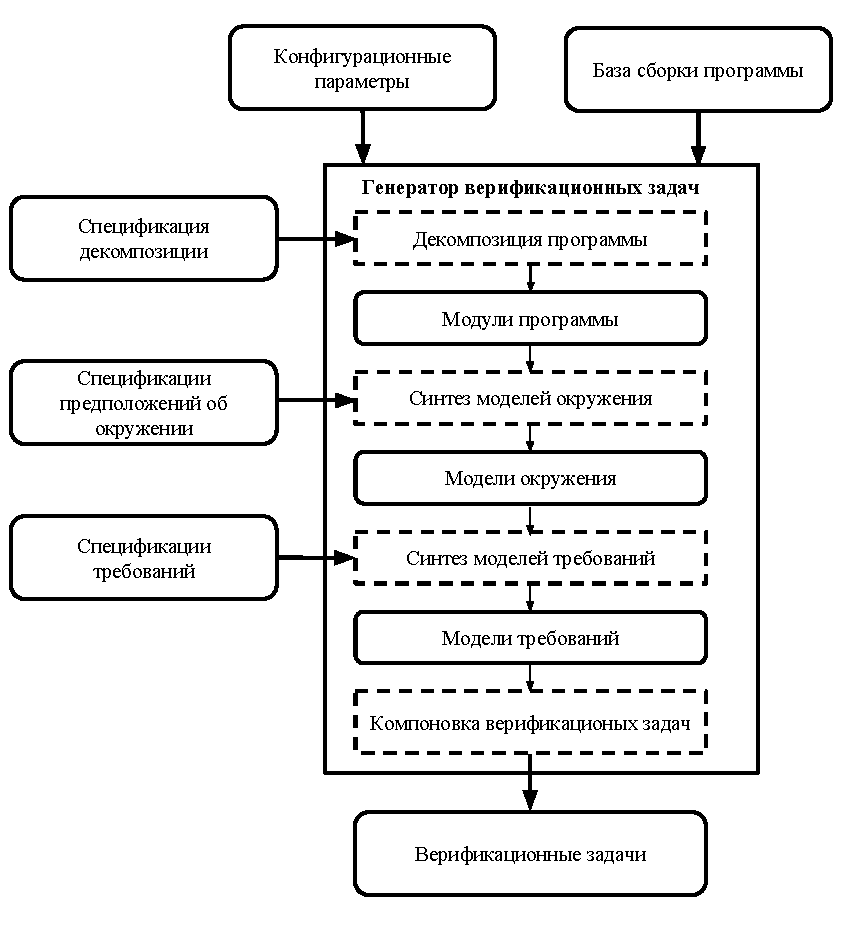
\includegraphics[scale=1]{vt_generator}
\caption{Схема генератора верификационных задач.}
\label{figure:vt_generator}
\end{figure}

Программные системы на языке Си, как правило, распространяются в виде файлов с исходным кодом и скриптов для их компиляции и компоновки.
Для получения информации об устройстве такой системы выполняется контролируемая сборка, в ходе которой подготавливается \textit{база сборки}.
В рамках данного метода процесс сбора такой базы не рассматривается и предлагается использовать для этого доступные инструменты.
База сборки должна содержать следующие данные в своем составе:
\begin{itemize}
    \item файлы с исходным кодом программной системы на языке программирования Си;
    \item команды компиляции и компоновки в виде графа зависимостей между командами сборки;
    \item описание программного интерфейса файлов программной системы.
    \end{itemize}
    
В базе сборки сохраняются все файлы программной системы с расширением <<.c>> и заголовочные файлы зависимостей, необходимые для выполнения препроцессирования.

Пример фрагмента графа зависимостей между командами сборки изображен на рисунке \ref{figure:cbg}.
Граф является ориентированным и его вершинам соответствуют файлы, которые являются входными и выходными файлами команд сборки, а ребра графа соответствуют самим командам сборки.
Граф должен включать не только команды компиляции и компоновки, но и команды перемещения, удаления, переименования файлов и т.п.
Наличие ребра в графе между двумя вершинами означает, что некоторая команда сборки принимает на вход исходный файл и получает на выходе новый файл.
В составе графа хранится вспомогательная информация о командах сборки, например, опции команд, путь к директории выполнения, значения переменных окружения.
Если граф построен корректно, то в графе нет ребер направленных к вершинам, которые соответствуют файлам с исходным кодом, а вершины, соответствующие финальным исполняемым файлам программной системы, не содержат исходящих ребер.

\begin{figure}
\centering
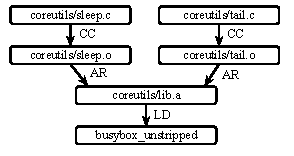
\includegraphics[scale=2]{cbg}
\caption{Фрагмент графа зависимостей команд сборки апплетов проекта BusyBox.}
\label{figure:cbg}
\end{figure}

Описание программного интерфейса программной системы представляет собой структурированные данные о составе каждого файла с исходным кодом, которые содержат:
\begin{itemize}
    \item Список деклараций и определений функций вместе с их сигнатурами.
    \item Граф вызова функций. Для каждого вызова должна быть сохранена информация о вызываемой и вызывающей функциях.
    Параметры вызова сохраняются в том случае, если среди них есть указатели на глобальные переменные или функции.
    \item Список инициализируемых глобальных переменных и их декларации.
    \item Список макросов и макроподстановок сохраняется аналогично списку определений и деклараций функций.
    \item Список определений и области видимости типов, определенных в программной системе.
\end{itemize}

Результатом работы генератора верификационных задач является набор верификационных задач в формате сообщества SV"~COMP.
Процесс генерации верификационных задач состоит из 4 шагов:
\begin{enumerate}
    \item На первом шаге в процессе декомпозиции определяются модули программной системы. 
    \item Затем для каждого модуля выполняется подготовка модели окружения на языке программирования Си.
    \item После моделей окружения синтезируются модели требований на языке программирования Си.
    \item Заключительным шагом является компоновка полученных на предыдущих шагах данных для получения верификационных задач в заданном формате.
\end{enumerate}

Каждый из перечисленных шагов выполняется отдельным компонентом генератора верификационных задач.
В рамках компонентов могут быть реализованы разные подходы и алгоритмы для выполнения конфигурирования в зависимости от проверяемых требований и программной системы.
Настройка процесса генерации верификационных задач выполняется согласно конфигурационным параметрам, заданным пользователем.

\section{Метод декомпозиции Си-программ на модули}
В данном разделе представлен метод автоматизированной декомпозиции Си-программ на модули, нацеленный на решение следующих задач:
\begin{itemize}
    \item выделить часть исходного кода программной системы, которую требуется верифицировать;
    \item декомпозировать выделенную часть исходного кода программной системы на модули, которые инструменты верификации моделей программ способны проверить по отдельности в составе верификационных задач.
\end{itemize}

Результат декомпозиции программной системы характеризуется следующими показателями:
\begin{itemize}
    \item \textit{Число полученных модулей}. Чем модулей меньше, тем, как правило, меньше времени потребуется на верификацию и ниже трудозатраты на моделирование окружения.
    \item \textit{Трудозатраты на моделирование окружения}. Трудозатраты зависят от сложности программного интерфейса модулей. Чем больше число точек входа и неопределенных функций в каждом модуле, тем больше моделей сценариев взаимодействия и неопределенных функций требуется подготовить пользователю.
    \item \textit{Число таких модулей, верификационные задачи на основе которых могут быть решены инструментом верификации моделей программ}.
\end{itemize}

Число точек входа и размер модулей лишь косвенно влияют на трудоемкость моделирования окружения и возможность решить верификационные задачи, построенные на основе модулей, в заданных ограничениях на вычислительные ресурсы при использовании определенного инструмента верификации моделей программ.
Трудоемкость моделирования окружения может оценить только пользователь, выполняющий верификацию, а вердикт станет известен только после непосредственного запуска инструмента верификации моделей программ.
Поэтому в данной работе предлагается выполнять процесс декомпозиции автоматически, но с возможностью конфигурирования и коррекции состава полученных модулей программы пользователем при помощи спецификации декомпозиции в зависимости от проверяемых требований и программы.

Для декомпозиции программной системы на языке Си предлагается выполнять следующие шаги:
\begin{enumerate}
    \item определить файлы и функции в составе программы;
    \item выделить модули;
    \item выбрать целевые модули;
    \item скорректировать состав модулей согласно спецификации декомпозиции;
    \item агрегировать модули.
\end{enumerate}

На шаге определения состава программы выполняется построение двух ориентированных графов на основе базы сборки: графа файлов и графа функций. 
Вершины графа функций соответствуют уникальным функциям, а ребро между вершинами присутствует в графе, если одна функция вызывается из другой.
Граф может не содержать тех функций, в которых нет вызова функций из других файлов программы и которые сами не вызываются за пределами файла с их определением.
Граф файлов строится таким образом, чтобы вершины соответствовали уникальным файлам с исходным кодом программы, а ребра связывали вершины, если хотя бы одна функция из файла вызывает некоторую функцию из другого файла.

На следующем шаге выполняется деление множества вершин графа файлов на непересекающиеся подмножества, согласно некоторой \textit{стратегии выделения модулей}.
При решении поставленной задачи могут использоваться данные из базы сборки, графа функций и графа файлов.
В результате декомпозиции должен быть получен граф модулей.
Вершиной графа является модуль программы --- это набор из одного или нескольких файлов программы.
Каждый файл программы должен быть частью некоторого модуля.
Между вершинами графа есть ребро, если есть хотя бы одно ребро в графе файлов между вершинами, которые соответствуют файлам из разных модулей.
Каждому модулю назначается уникальное имя.
Требуется, чтобы при верификации одной и той же версии программы с одними и теми же конфигурационными параметрами алгоритм получал всегда один и тот же граф модулей с одними и теми же именами вершин и составом каждого модуля.

Для каждой новой верифицируемой программы предлагается разрабатывать подходящую стратегию выделения логических компонентов.
Архитектура компонента декомпозиции программ должна позволять выделять общие между реализациями стратегий алгоритмы и функции, чтобы сократить трудоемкость разработки.

Шаг выделения модулей является необязательным и может быть пропущен на начальной стадии выполнения верификации или при проверке программ небольшого размера, для которых состав модулей нетрудно задать вручную при помощи спецификации декомпозиции.

Задачу декомпозиции графа файлов можно свести к строго математической задаче разбиения множества вершин графа на подмножества и использовать для ее решения различные существующие алгоритмы, не опирающиеся на особенности устройства декомпозируемых программных систем.
Данный подход может быть реализован в качестве одной из стратегий выделения модулей в рамках данного метода.
Трудность такого подхода заключается в определении способа формализации данной задачи таким образом, чтобы ее решение действительно способствовало улучшению показателей применимости метода на практике, то есть снижению показателя трудоемкости моделирования окружения и повышению числа верификационных задач, подготовленных на основе модулей, для которых возможно получить вердикт при заданных ограничениях на вычислительные ресурсы. 
Так как набора таких характеристик модуля, которые явно влияют на целевые показатели, предложить не удается, то и разные алгоритмы решения данной задачи оказываются применимы только в некоторых частных случаях.

Следующим шагом является выбор целевых модулей.
Пользователь в числе конфигурационных параметров может перечислить два списка имен директорий, файлов, функций или модулей.
Списки могут содержать и регулярные выражения для определения таких имен.
Один список перечисляет те объекты, которые требуется верифицировать, а другой те, которые верифицировать не требуется.
На шаге выбора целевых модулей должны быть помечены вершины графа модулей, которые требуется верифицировать на основе данных списков.
Для каждого заданного пользователем элемента списка определяется соответствующее множество целевых файлов: для директории все файлы с исходным кодом, включая и файлы из поддиректорий, для модулей все файлы из их состава, а для функции файл с ее определением.
Затем формируется множество целевых файлов, предназначенных для верификации, а затем из него вычитается множество элементов, полученных для списка имен объектов, которые следует исключить.
В результате должно быть сформировано непустое множество целевых файлов, которые требуется верифицировать, и каждая вершина графа файлов, соответствующая элементу данного множества, помечается как целевая.
Каждая вершина графа модулей тоже помечается как целевая, если соответствующий модуль содержит хотя бы один целевой файл.

Затем выполняется шаг коррекции состава модулей, который является необязательным и выполняется в том случае, если пользователь подготовил спецификацию декомпозиции.
Спецификация декомпозиции может содержать следующие команды:
\begin{itemize}
    \item Добавить или заменить состав файлов модуля с определенным именем.
    \item Добавить или удалить определенные файлы из модуля с некоторым именем.
    \item Удалить определенные файлы из всех модулей.
    \item Добавить определенные файлы ко всем модулям.
\end{itemize}

Для удобства пользователя следует предоставить возможность задавать не только имена файлов, но и функций, логических компонентов и директорий, а также поддержать использование регулярных выражений при задании спецификации декомпозиции.

На основе заданной пользователем спецификации декомпозиции выполняется коррекция вершин графа модулей, а затем на основе графа файлов заново определяются множества ребер графа модулей и его целевые вершины. 

Последним шагом является агрегация модулей.
На данном шаге выполняется для каждого целевого модуля поиск наборов модулей, которые могут включать и нецелевые модули, согласно некоторой \textit{стратегии агрегации}.
Стратегия реализует алгоритм для выбора модулей, чтобы либо снизить число точек входа целевого модуля, либо снизить число неопределенных функций при объединении модулей из набора в новый модуль.
Агрегация нацелена на сокращение трудоемкости моделирования окружения при помощи верификации модулей вместе.
При разработке стратегии стоит учесть, что увеличение числа наборов объединенных модулей приводит к увеличению времени верификации, а увеличение размера наборов повышает риск возникновения взрыва числа состояний в модели, построенной инструментом верификации на основе исходного кода объединенных модулей.

В рамках предложенного метода предлагается разработать несколько стратегий агрегации на основе различных алгоритмов.
Стратегии могут опираться не только на графы модулей, файлов и функций, но и на некоторую вспомогательную информацию, которую может предоставить пользователь.
Например, такими данными могут быть отчеты о покрытии, полученные при верификации модулей по-отдельности.

Каждый набор модулей, полученный в ходе агрегации, становится новым модулем, для которого затем выполняется синтез моделей окружения и требования.

\begin{figure}
\centering
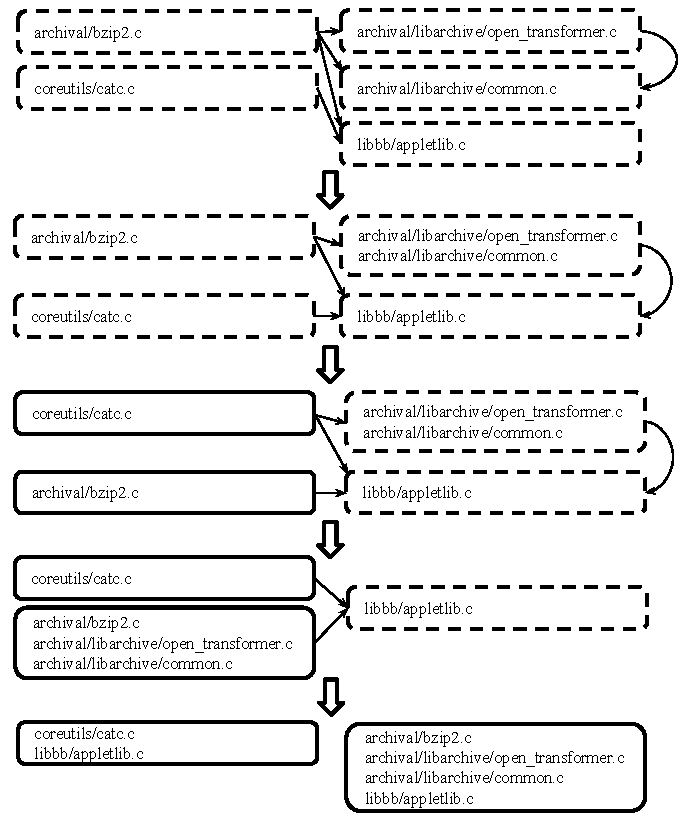
\includegraphics[scale=1.2]{decomposition_example}
\caption{Пример декомпозиции фрагмента проекта BusyBox на модули.}
\label{figure:decomposition_example}
\end{figure}

Рассмотрим процесс декомпозиции на примере, представленном на рисунке~\ref{figure:decomposition_example} и основанном на небольшой части проекта BusyBox.
Пример иллюстрирует результат работы каждого шага метода.
Прямоугольниками со сплошными границами представлены целевые модули, а нецелевые модули имеют пунктирные границы.
Стрелки соответствуют зависимостям по вызову функций между файлами и модулями.
\begin{itemize}
    \item Пусть после выполнения определения состава программы оказалось, что в программе 5 файлов, зависимости по вызову функций между которыми представлены на рисунке. 
    В данном примере файлы в левой части соответствуют апплетам \textit{bzip2} и \textit{catc}, каждый из которых имеет свою функцию \textit{main}.
    Файл из директории \textit{libbb} соответствует одноименной библиотеке функций, которая может быть использована любым апплетом.
    Файлы из директории \textit{archival/libarchive} реализуют вспомогательные функции для различных апплетов, предназначенных для сжатия и распаковки архивов.
    \item На втором шаге выполняется выделение модулей на основе некоторой стратегии.
    Пусть в данном примере стратегия на основе графа вызова функций предполагает объединение файлов из одной директории, отделяя друг от друга те модули, в которых в каждом есть своя функция \textit{main}.
    \item На третьем шаге выбираются целевые модули.
    В данном случае целевыми являются модули с файлами \textit{bzip2} и \textit{catc}, которые содержат функции \textit{main}.
    \item На предпоследнем шаге выполняется коррекция состава модулей согласно спецификации декомпозиции.
    Предположим, что пользователь указал, что для всех апплетов из \textit{archival} необходимо добавить файлы из\break \textit{archival/libarchive}, которые в свою очередь не нужно выделять в отдельный модуль.
    \item На заключительном этапе на основе графа вызова функций между модулями для сокращения затрат на моделирование окружения выполняется агрегация апплетов со вспомогательной библиотекой \textit{libbb}.
\end{itemize}

Предложенный метод позволяет адаптировать процесс декомпозиции для проверки различных программных систем на языке программирования Си.
Для этого предлагается разрабатывать стратегии выделения модулей и агрегации, а также спецификации декомпозиции.

\section{Метод спецификации моделей окружения}
В данном разделе представлен метод спецификации моделей окружения модулей на основе систем переходов.

\subsection{Промежуточная модель окружения}
После декомпозиции программы требуется для каждого модуля Си-программы подготовить модель окружения, которая состоит из моделей неопределенных функций и моделей сценариев взаимодействия.

Для преобразующих программ с функцией \textit{main} не требуется описывать разные последовательности вызова точек входа и прежде всего нужно разработать модели определенных в окружении функций на языке программирования Си.
В данной работе внимание сосредоточено именно на задаче моделирования сценариев взаимодействия, в которых выполняется вызов точек входа модулей.

Процесс моделирования окружения для библиотек и событийно-ориентированных программ требует построения композиции из отдельных моделей сценариев взаимодействия.
Объединение модулей программы при использовании стратегий агрегации ведет, как правило, к уменьшению трудозатрат на моделирование.
Однако при этом могут возникать новые ограничения на последовательности событий из разных сценариев взаимодействия.
Способ описания таких требований не должен препятствовать раздельной верификации модулей с одними и теми же моделями сценариев, то есть реализации таких моделей не должны существенным образом зависеть друг от друга.
Для решения данной задачи в настоящей работе предлагается метод задания моделей сценариев на основе систем переходов.
Спецификацию предположений об окружении для некоторого модуля программы, подготовленную при помощи данного метода, назовем промежуточной моделью окружения.

Способ описания промежуточной модели окружения должен удовлетворять ряду требований для удобства применения на практике:
\begin{itemize}
    \item Модели сценариев взаимодействия должны быть описаны отдельно друг от друга.
    \item Модели событий следует описывать на языке программирования Си. 
    Такой подход призван облегчить восприятие моделей пользователем и упростить их трансляцию на язык Си при подготовке финальной модели окружения.
    \item При агрегации нескольких модулей модель окружения в промежуточном представлении для группы модулей должна быть построена как параллельная композиция моделей сценариев, подготовленных для отдельных модулей.
    Каждая модель сценария описывает события взаимодействия, которые происходят в отдельном потоке окружения согласно семантике выполнения многопоточной программы в соответствии со стандартом POSIX.
\end{itemize}

Рассмотрим способ задания промежуточной модели окружения, не опираясь на конкретный синтаксис, который может быть реализован по-разному.
Пусть требуется разработать модель окружения для модуля программы на языке программирования Си с программным интерфейсом $I = <V_p, F_p, R_e, T_e>$, который содержит множества глобальных переменных, функций, макросов и типов, для которых известны сигнатуры, область видимости в файлах программы и файл с объявлением или определением.
Описание программного интерфейса может быть получено из базы сборки программы.

Промежуточную модель окружения данного модуля обозначим как $M$, где:
\[ M = <V_e, F_e, R_e, T_e, E> \]
Здесь $V_e, F_e, R_e, T_e$ --- это множества вспомогательных вспомогательных переменных, функций, макросов и типов.
Для переменных заданы объявления и инициализаторы, а для остальных элементов даны определения на языке программирования Си.
Пересечения перечисленных множеств с соответствующими множествами из $I$ могут быть непустыми.
$E$ содержит конечное множество моделей сценариев взаимодействия модуля программы и окружения.

Множество $F_e$ содержит определения моделей функций из окружения и \textit{служебных функций}.
Множества $R_e, T_e$ и $V_e$ являются вспомогательными и необходимы для реализации моделей функций окружения и моделей сценариев взаимодействия.
Служебные функции выполняют следующие задачи:
\begin{itemize}
    \item При помощи данных функций может быть выделена общая функциональность ряда моделей.
    \item Служебные функции могут реализовывать модели функций стандартной и других библиотек, которые необходимы при использовании определенных инструментов верификации моделей программ.
    К таким функциям относятся функции выделения памяти, работы со строками, механизмами синхронизации и др.
    \item Некоторые служебные функции служат для <<связывания>> моделей окружения и моделей требований. Подробнее этот вопрос рассматривается в разделе, посвященном синтезу моделей требований.
\end{itemize}

Множество моделей сценариев взаимодействия $E$ содержит модели сценариев, которые делятся на два вида: модели функций окружения и модели потоков окружения. 
Каждая модель функции окружения реализует модель сценария взаимодействия, события которого происходят во время выполнения некоторой функции окружения из $F_p \setminus F_e$. 
Модель потока окружения реализует модель сценария, события которого выполняются
в некотором отдельном потоке окружения.
Все модели потоков окружения в точке входа модели окружения начинают выполнение одновременно.

Каждая модель сценария определяется четверкой:
\[ \varepsilon = <\mathcal{V}, \mathcal{A}, \alpha_0 ,\mathcal{R}>\]
Где $\mathcal{V}$ --- это множество переменных состояния, а $\mathcal{A}$ --- это множество \textit{действий} $\mathcal{R}:~ \mathcal{A}~\times~\mathcal{A}$ --- отношение переходов, описывающее допустимый порядок следования действий.

Модель сценария всегда начинается с выполнения действия $\alpha_0$, а последующие действия определяются отношением переходов $\mathcal{R}$. 
Будем различать действия трех видов: \textit{прием} и \textit{отправка} сигналов, а также \textit{модели событий}.

Модели событий предназначены для вызова точек входа и выполнения операций с их параметрами.
Модель события определяется тройкой:
\[\alpha = <\varphi, \beta, \psi> \]
Где $\beta$ --- это базовый блок кода на языке программирования Си, состоящий из операций над переменными $\mathcal{V} \cup V_p \cup V_e$, в котором могут быть вызваны функции из $F_p$ и $F_e$.
Базовый блок должен содержать корректный код и иметь один вход и один выход, то есть, если в блоке есть операторы ветвления или циклов, то они полностью должны входить в состав блока.
В базовых блоках запрещено объявлять новые переменные и использовать оператор $goto$.
Логические выражения $\varphi$ и $\psi$ на языке программирования Си над переменными $\mathcal{V}_i \cup V_p \cup V_e$ описывают предусловия и постусловия действия.

Действия передачи сигналов служат для описания зависимостей по порядку и данным между моделями событий из разных сценариев.
Рассмотрим модель сценария $\varepsilon_i$ с действием отправки сигнала и модель сценария $\varepsilon_j$ с действием получения сигнала.
Соответствующие действия $\alpha_i \in \mathcal{A}_i$ и $\alpha_j \in \mathcal{A}_j$ имеют вид:
\begin{align*}
&\alpha_i = <\varphi_i, \varepsilon_i, l_m>
&\alpha_j = <\varphi_j, \pi_j, l_n, \psi_j>    
\end{align*}
Константы $l_m$ и $l_n$ называются именами сигналов.
Передача сигнала возможна только тогда, когда в соответствующих действиях отправки и получения указано одно и то же имя сигнала $l_m = l_n$.
Логические выражения $\varphi_j$ и $\psi_j$ на языке программирования Си над переменными из $\mathcal{V}_j \cup V_p \cup V_e$ определяют предусловие и постусловие приема сигнала.
Предусловие посылки сигнала является логическим выражением $\varphi_i$, определенным на множестве переменных $\mathcal{V}_i \cup V_p \cup V_e$.
Два набора переменных $\varepsilon_i: {v_1, ..., v_k}$ где $t = 1..k, v_t \in \mathcal{V}_i$ и $\pi_j: {u_1, ..., u_k}$ где $t = 1..k, u_t \in \mathcal{V}_j$ предназначены для передачи значений между переменными состояния отправителя и получателя:
\begin{align*}
&\forall t = 0..k:~v_t := u_t
\end{align*}
Типы переменных должны либо совпадать, либо допускать преобразование.

Посылка сигнала происходит между одним получателем и одним отправителем согласно модели синхронизации потоков рандеву, предложенной в работе~\cite{Hoare:1978:CSP}.
Передача происходит между двумя моделями сценариев, одна из которых отправляет сигнал, а другая получает, причем имя сигнала в заданных действиях должно совпадать.
Для этого получатель должен выполнить действие получения сигнала, разрешенное отношением переходов, а отправитель выполнить соответствующее действие посылки сигнала.
Как только и отправитель, и получатель начали выполнять соответствующие действия, то может быть произведена передача данных.
После передачи данных отправитель может продолжать выполнение других действий, а получатель продолжит свою работу только после получения данных, которое может произойти не одновременно с отправкой.
Отправитель или получатель могут предпринять и другие действия, допустимые отношением переходов, независимо от наличия потенциальных получателей или отправителей.
Если же отношение переходов не разрешает выполнение других действий кроме посылки или отправки сигнала, то никаких действий в модели сценария выполняться не должно до появления необходимой пары для передачи сигнала.
Если потенциальных получателей или отправителей несколько, то пересылка сигнала происходит согласно недетерминированному выбору двух участников, а остальные модели сценариев, которые должны выполнить посылку или отправку сигнала с тем же именем, ожидают завершения передачи сигнала.

Модели сценариев можно описывать на языке программирования Си, как и остальные части промежуточной модели окружения $M$.
В этом случае каждая модель сценария может быть определена при помощи функции, в которой будут объявлены переменные состояния, а порядок действий может быть задан при помощи операторов языка.
Для действий посылки и получения сигналов предлагается расширить язык Си вспомогательными операциями для удобства спецификации.
Но и данные операции можно транслировать на язык Си, что будет описано в следующем разделе.
При реализации метода синтеза моделей окружения для задания моделей сценариев промежуточной модели окружения могут быть использованы и дополнительные расширения языка Си для решения ряда задач, возникающих на практике для преодоления ограничений инструментов верификации моделей Си-программ.

При спецификации промежуточной модели окружения целесообразно использовать специальные поддерживаемые инструментами верификации функции.
Поэтому исходный код модели окружения не предназначен для выполнения и служит только для компоновки с исходным кодом модуля программы в рамках верификационной задачи.

Семантика выполнения модели окружения без исходного кода модуля не имеет смысла, так как модель окружения предназначена для того, чтобы дополнить исходный код модуля до структурно-полной программы на языке Си.
В такой программе только одна точка входа и неопределенными могут быть только некоторые функции стандартной библиотеки и те функции, для которых инструмент верификации имеет встроенную модель.

\subsection{Пример промежуточной модели окружения}
Рассмотрим пример промежуточной модели окружения для модуля подсистемы.
Для задания моделей сценариев промежуточной модели окружения будем использовать язык Си, в котором будут добавлены расширения для обозначения действий передачи и получения сигналов.
Операции для посылки и приема сигнала $A$ пусть имеют вид $send(A, p1, ..., pN);$ и \break $receive(A, p1, ..., pN);$ соответственно.
Порядок действий будем задавать при помощи условного оператора и функции \textit{\_\_VERIFIER\_nondet\_int}, а предусловия и постусловия будут заданы при помощи функции \textit{\_\_VERIFIER\_assume}.
Такой способ несколько затрудняет восприятие, зато позволяет строго обозначить начало и конец описания каждого действия, которые будем сопровождать соответствующими комментариями.

Для данного модуля был предложен пример модели окружения, которая состояла из моделей сценария вызова библиотечных функций и сценария инициализации подсистемы.
Модель сценария инициализации подсистемы пусть имеет вид:

\begin{lstlisting}[language=C,basicstyle=\small]
void init_scenario(void) {
    // State vars
    int ret;

    // Transition Relation    
    // Block Action 1 begin
    ret = tty_init();
    // Block Action 2 end
    if (__VERIFIER_nondet_int()) {
        // Send Action 2 begin
        __VERIFIER_assume(ret == 0);
        send("INITIALIZED");
        // Send Action 2 end
    }
}
\end{lstlisting}

Здесь при помощи комментариев на языке Си обозначены конкретные части описания сценария: переменные состояния, операторы отношения переходов и действия.
Первое действие является блоком кода, в котором выполняется вызов функции инициализации подсистемы.
А второе действие с предусловием, выраженным при помощи вызова функции \textit{\_\_VERIFIER\_assume}, отправляет сигнал для активации сценария вызова библиотечных функций, который в свою очередь может быть задан следующим образом:

\begin{lstlisting}[language=C,basicstyle=\small]
void functions_scenario(void) {
    // State vars
    int ret;
    struct tty_driver *driver;
    struct tty_operations *ops;
    
    // Transition Relation
    // Receive Action 1 begin
    receive("INITIALIZED");
    // Receive Action 1 end
    // Block action 2 begin
    driver = tty_alloc_driver(...)
    // Block action 2 end
    if (__VERIFIER_nondet_int()) {
        // Block action 3 begin
        __VERIFIER_assume(driver != 0);
        ops = __VERIFIER_nondet_pointer();
        tty_set_operations(driver, ops);
        // Block action 3 end
        // Block action 4 begin
        ret = tty_register_driver(driver)
        // Block action 4 end
        if (__VERIFIER_nondet_int()) {
            // Send Action 5 begin
            __VERIFIER_assume(ret == 0);
            send("Register TTY callbacks", driver);
            // Send Action 5 end
            // Receive Action 6 begin
            receive("Unregister TTY callbacks", driver);
            __VERIFIER_assume(driver->ops == ops);
            // Receive Action 6 end
            // Block action 7 begin
            tty_unregister_driver(driver);    
            put_tty_driver(driver);
            // Block action 7 end
        } else {
            // Block action 8 begin
            __VERIFIER_assume(ret != 0);
            // Block action 8 end
        }
    }    
}
\end{lstlisting}

Первым действием сценария является прием сигнала, который означает, что подсистема инициализирована.
Затем выполняется вызов точек функций подсистемы.
Отличительной особенностью данной модели по сравнению с моделью окружения на языке Си, которая была предложена в первом разделе данной главы, является посылка и ожидание сигналов \textit{Register TTY callbacks} и \textit{Unregister TTY callbacks} после успешного вызова функции \textit{tty\_register\_driver}.
Данные действия указаны для демонстрации того, как указание о возможности вызова обработчиков драйверов может быть передано соответствующим моделям сценариев.
Данная модель сценария ожидает сигнал \textit{Unregister TTY callbacks}, который означает, что вызов обработчиков драйверов завершен.
Если в промежуточной модели окружения нет моделей сценариев, которые отправляют или принимают сигналы \textit{Register TTY callbacks} и \textit{Unregister TTY callbacks}, то они могут быть удалены из рассматриваемой модели вызова библиотечных функций при трансляции на язык Си.

\subsection{Трансляция промежуточных моделей окружения}
Модели сценариев, согласно предложенному методу, можно описывать на языке программирования Си, но для описания действий посылки и получения сигналов предлагается расширить язык Си вспомогательными операциями для удобства спецификации.
Поэтому промежуточные модели окружения должны быть предварительно транслированы на язык программирования Си. 
Тогда нужно показать, что трансляция промежуточной модели окружения не влияет на возможность обнаружения ошибок в модуле.

Модель окружения на языке программирования Си анализируется в рамках верификационной задачи инструментом верификации моделей программ при проверке некоторого свойства корректности.
Под программой далее будем понимать именно совокупность исходного кода модели окружения и модуля программы.
По исходному Си-программы строится модель, которая проверяется на соответствие свойству недостижимости ошибочных состояний\footnote{В данной работе рассматриваются только такие свойства корректности, которые могут быть сведены к задаче недостижимости ошибочного оператора.} методом верификации моделей.
Покажем, что множества ошибочных состояний исходной программы и программы, полученной после трансляции исходной программы на язык Си, изоморфны.
Для этого необходимо рассмотреть свойства таких моделей рассматриваемых программ, которые используются инструментами верификации моделей при проверке свойств недостижимости ошибочного оператора.

\subsubsection{Символическая система переходов}

Для описания моделей программ воспользуемся символическими системами переходов (англ. symbolic transition system)~\cite{Clarke:1981}.
Система определяется тройкой $STS \mathbf{:=} <V, \alpha, \delta>$. Где $V$ --- конечное множество типизированных переменных системы, каждая из которых задана на дискретном конечном множестве значений.
Функция означивания $s \in \Sigma_V$ переменных из множества $V$ называется состоянием системы. Множество $\Sigma_V$ --- это множество состояний системы, полученное перебором всех возможных значений переменных из множества $V$.
Формула пропозициональной логики $\alpha(V)$ над переменными из множества $V$ называется \textit{характеристической функцией множества начальных состояний}.
Состояния, при которых данный предикат принимает истинное значение, называются \textit{начальными состояниями}.
Формула пропозициональной логики $\delta(V, V^{'})$ --- это \textit{характеристическая функция отношения переходов} между состояниями.
Функция определена над переменными из $V \cup V^{'}$, то есть переменными в данном и в следующем состояниях системы.
Если для двух состояний $s_1 \in \Sigma_V$ и $s_2 \in \Sigma_V$ выполняется $(s_1, s_2) \models \delta$, то между ними возможен переход.

\textit{Путь} --- это конечная последовательность $\xi_k = s^0, s^1, ..., s^k$ состояний \break $s^{i} \in \Sigma_{V}$, в которой для каждого состояния справедливо $(s^{i}, s^{i+1}) \models \delta$ и для начального состояния $s^1 \models \alpha$. 
\textit{Предикат пути} длины $k$ шагов имеет вид:

\[
\eta_k \mathbf{:=} \alpha(V^{1}) \land \bigwedge_{i \in [1,k]}\delta[V = V^{i}, V^{'} = V^{i+1}](V, V^{'})
\]

$V^{i}$ обозначает множество переменных системы на шаге выполнения $i$.
Будем говорить, что состояние $s^k \in \Sigma_{V}$ достижимо за $k$ шагов, если существует такой путь выполнения $\xi_k = {s^1, s^2, ... s^k}$, что $\xi_k \models \eta_k$.
Обозначим множество всех достижимых за $k$ шагов состояний как $R_k$, а множество всех достижимых состояний как $R$.

Рассмотрим некоторое подмножество переменных системы $U \subseteq V$.
Проекцией состояния $s \in \Sigma_{V}$ на множество переменных $U$ называется такая функция означивания переменных $U$, обозначаемая как $s \Downarrow U$, которая переменным из $U$ ставит в соответствие те же значения, что и $s$.
Проекцией $K \Downarrow U$ некоторого подмножества всех состояний системы $K \subseteq \Sigma_V$ на множество переменных $U$ назовем множество всех проекций состояний из $K$ на множество переменных $U$.


\subsubsection{Символическая система переходов и структуры Крипке}
Каждый способ моделирования систем <<фиксирует>> свой набор свойств системы.
Метод описания систем при помощи структур Крипке широко распространен и применяется в том числе и для проверки свойства недостижимости ошибочных состояний.
Метод моделирования систем при помощи систем символических переходов не уступает в выразительности структурам Крипке.

Построим следующую структуру Крипке про произвольной $STS$:
\[K \mathbf{:=} <S, S_0, R, L>\]

\begin{itemize}
    \item $S = \Sigma_V$ --- конечное множество абстрактных состояний, полученное путем рассмотрения всех значений переменных $V$.
    \item $S_0 = \{s \in S| s \models \alpha\}$ --- множество начальных состояний, удовлетворяющих характеристической функции $\alpha$.
    \item $R = \{(s, t)| (s, t) \models \delta\}$ --- отношение переходов, которое определяется определяется характеристической функцией $\delta$.
    \item $L(s)$ --- такая функция разметки, которая ставит в соответствие состоянию набор истинных предикатов из $AP = \{a_1, ..., a_k\}$, определенных на множестве переменных $V$. То есть $a_i \in L(s)$, если $s \models a_i$.
\end{itemize}

В построенной структуре Крипке $K$ и в $STS$ множества всех состояний системы, начальных состояний и переходов попарно совпадают.
То есть для любой символической системы переходов может быть построена эквивалентная структура Крипке.

\subsubsection{Язык программирования $LZ$}

Расширения языка Си для отправки и получения сигналов влияют на порядок выполнения операций в программе и передачу данных между потоками.
Предположим, что и при трансляции новых операций на язык Си будут использоваться некоторые только операции с целыми числами, захват и освобождение блокировок, проверка простых логических выражений.
При посылке и получении сигналов, а также при трансляции данных операций на язык Си, не предполагается использовать вызовы произвольных функций, циклы с переменным числом итераций, рекурсию, изменять значения по указателям, выделять или освобождать память, создавать или останавливать потоки, выполнять переходы по goto и т.п.
Поэтому при рассмотрении программ и их моделей целесообразно рассмотреть упрощенный Си-подобный язык, который сохранит именно те особенности семантики программ на языке Си, на которые влияет добавление операций посылки и получения сигналов.
Таким языком станет некоторый структурный статически типизированный язык программирования $LZ$.

Программа на языке $LZ$ имеет следующий синтаксис:
\begin{flalign*}
& Globals:~g_1:~\tau_1;~g_2:~\tau_2;~...~g_n:~\tau_n;\\
& Procedures: \\
& ~~~Procedure~1:\\
& ~~~~~~Locals:~v_1:~\tau_1;~v_2:~\tau_2;~...~v_{k_1}:~\tau_{k_1}; \\
& ~~~~~~P_1; \\
\\
& ~~~Procedure~2:\\
& ~~~~~~Locals:~v_2:~\tau_1;~v_2:~\tau_2;~...~v_{k_2}:~\tau_{k_2}; \\
& ~~~~~~P_2; \\
& ~~~... \\
& ~~~Procedure~N:\\
& ~~~~~~Locals:~v_2:~\tau_1;~v_2:~\tau_2;~...~v_{k_N}:~\tau_{k_N}; \\
& ~~~~~~P_N; \\
\end{flalign*}

Здесь использовались следующие обозначения:
\begin{itemize}
    \item $g_i$ --- глобальные переменные программы с типами $\tau_i$. Множества значений типов $\{int, lock, bool\}$ являются конечными и дискретными. Тип $int$ соответствует подмножеству целых чисел, $bool$ соответствует истинностным значениям, множество значений типа $lock$ содержит два элемента: 0 (блокировка не захвачена) и 1 (блокировка захвачена). \item $Procedure~i$ --- заголовок описания процедуры с номером $i$, которое состоит из деклараций локальных переменных $v_i$ и кода $P_i$ процедуры.
\end{itemize}

Выполнение программы представляет собой параллельное выполнение операций из процедур программы в отдельных потоках. 
Каждый $i$-ый поток выполняет соответствующую ему процедуру $P_i$.
Потоков в программе всегда не менее 1 и все они начинают выполнение одновременно.
Порядок выполнения операций одной процедуры определяется операторами следования ($;$), ветвления ($if$) и цикла ($while$).

Грамматика кода процедуры $P_i$ имеет вид:
\begin{flalign*}
P \mathbf{:=} &~P;P~|~if~(A)~\{P\}~else~\{P\}~|~while~(A)~\{P\}~|~op~|~skip \\
op \mathbf{:=} &~x = t~|~lock(x)~|~unlock(x)~|~assume(A) \\
t \mathbf{:=} &~(t)~|~t - t~|~x~|~t + t \\
A \mathbf{:=} &~\neg A~|~A \land A~|~A \lor A~|~A \to A~|~(A)~|~x~|~nondet()
\end{flalign*}

Рассмотрим каждый символ подробнее:
\begin{itemize}
    \item $op$ --- операция в программе. Операциями являются $lock$, $unlock$, $assume$, $skip$ и присваивание.
    \item t --- выражение, составленное при помощи арифметических операторов \{+, -\} над переменными программы с типом $int$. Выражения используются только в операциях присваивания.
    \item x --- имя некоторой переменной. В любой процедуре может выполняться доступ к глобальным переменных и локальным переменным данной процедуры. Локальные переменные могут иметь только типы $int$ и $bool$.
    \item $lock(x)$ и $unlock(x)$ --- функции захвата и освобождения блокировки $x$. Блокировками являются глобальные переменные с типом $lock$.
    \item nondet() --- неопределенное значение из множества значений типа $bool$;
    \item $A$ --- логическая формула пропозициональной логики, расширенная теорией целых чисел. Формула может быть составлена при помощи логических связок $\{!, \&\&, ||, ==\}$ над переменными программы;
    \item $assume(A)$ --- проверка выполнения формулы $A$. Если формула не истинна, то процедура не может продолжить выполнение и перейти к следующей операции.
    \item $skip$ --- операция бездействия.
\end{itemize}

\subsubsection{Модель программ на языке программирования $LZ$}
Построим модель программы $P$ на языке $LZ$ при помощи символической системы переходов $STS \mathbf{:=} (V_P, \alpha_P, \delta_P)$.

В каждой процедуре пронумеруем каждую операцию и проверку условий циклов и операторов ветвления.
В результате каждая операция и условие операторов цикла или ветвления будут иметь свой уникальный порядковый номер, называемый \textit{меткой}.
Дополнительной меткой обозначим конец каждой процедуры.

Введем следующие обозначения:
\begin{itemize}
    \item $V_P = V \cup PC$--- множество переменных состояния.
    \item $\Sigma_{V_P}$ --- множество всех состояний модели программы.
    \item $V = G \cup L_0 \cup ... \cup L_N$ --- множество переменных.
    \item $G$ --- множество глобальных переменных программы.
    \item $L_i$ --- множество локальных переменных процедуры с номером $i$. 
    $V_i = G \cup L_i$ --- множество переменных процедуры $i$.
    \item Переменные $pc_i$ (англ. program counter) являются вспомогательными и предназначены для сохранения метки текущей выполняемой операции или проверяемого условия оператора. Множество таких переменных обозначим как $PC = \{pc_1, ... , pc_N\}$. 
    Элементы множества $C \subset \Sigma_{PC}$ всех допустимых функций означивания переменных $PC$ будем называть конфигурациями, а $\Sigma_{PC}$ множеством конфигураций.
    \item $\alpha_{P}(V_P)$ --- характеристическая функция начальных состояний.
    \item $\delta_{P}(V_{P}, V^{'}_{P})$ --- характеристическая функция отношения переходов.
\end{itemize}
 
Выполнение программы будем моделировать как асинхронную параллельную композицию потоков.
Характеристическая функция отношения переходов имеет вид:

\begin{flalign*}
& \delta_P(V_P, V^{'}_P) \mathbf{:=} \bigvee_{i \in [1,N]}(\delta_{i}(V_i, pc_i, V^{'}_i, pc_i^{'}) \land \sigma_i)\text{, где}  
\\
& \sigma_i \mathbf{:=} \bigwedge_{\substack{j \in [1,N],\\j \neq i}}same(\{pc_j\}\cup L_j)
\end{flalign*}

Здесь предикат $same(A)$ означает, что переменные из некоторого подмножества переменных состояния $A \subset V_P$ сохраняют свои значения:

\[same(A) \mathbf{=} \bigwedge_{x \in A}x^{'} = x\]

\textit{Характеристическая функция процедуры} $\delta_{i}(V_i, pc_i, V_i^{'}, pc_i^{'})$ моделирует выполнение отдельного потока с номером $i$.
Пусть поток выполняет процедуру $P_i$, в которой $k_i$ меток, тогда: 

\begin{align*}
\delta_{i}(V_i, pc_i, V^{'}_i, pc_i^{'}) \mathbf{:=} \bigvee_{l \in [1,k_i]}\delta_{op_l}(V_i, pc_i, V^{'}_i, pc_i^{'})
\end{align*}

Где $\delta_{op_l}$ --- \textit{характеристическая функция операции или оператора с меткой $l$}.
Пусть операция имеет метку $l_1$, а метка следующей выполняемой операции или условия оператора будет $l_2$.
Тогда характеристическая функция операции в позиции $l_1$ имеет вид:

\begin{align*}
\delta_{op_{l_1}}(V_i, pc_i, V'_i, pc'_i) \mathbf{:=} pc_i = l_1 \land pc'_i = l_2 \land \rho_{op}(V_i, V'_i)
\end{align*}

Здесь $\rho_{op}(V_i, V'_i)$ --- \textit{характеристическая функция операции}, которая не зависит от метки.
Характеристические функции операций языка представлены в таблице~\ref{table:predicate}.
 
Рассмотрим проверку условия $A(V_i)$ оператора ветвления или цикла с меткой $l_1$.
Если условие истинно, то выполнеются операция с меткой $l_{true}$, а иначе операция с меткой $l_{false}$.
Тогда характеристическая функция условия оператора с меткой $l_1$ имеет вид:

\begin{align*}
\delta_{op_{l_1}}(V_i, pc_i, V'_i, pc'_i) \mathbf{:=} & pc_i = l_1 \land same(V_i) \land \\
& (A(V_i) \land pc' = l_{true} \lor \neg A(V_i) \land pc' = l_{false})
\end{align*}

\begin{table}
\centering
\begin{tabular}{ | l | l |}
\hline
Операция & Характеристическая функция \\
\hline
$lock(x)$ & $\rho_{op}(V_i, V'_i) \mathbf{:=} x = 0 \land x' = 1 \land same(V_i \setminus \{x\}))$ \\
\hline
$unlock(x)$ & $\rho_{op}(V_i, V'_i) \mathbf{:=} x' = 0 \land same(V_i \setminus \{x\})$ \\
\hline
$x = t(V_i)$ & $\rho_{op}(V_i, V'_i) \mathbf{:=} x' = t(V_i) \land same(V_i \setminus \{x\})$ \\
\hline
$assume(A(V_i))$ & $\rho_{op}(V_i, V'_i) \mathbf{:=} A(V_i) \land same(V_i)$ \\
\hline
$skip$ & $\rho_{op}(V_i, V'_i) \mathbf{:=} same(V_i)$ \\
\hline
\end{tabular}
\caption{Характеристические функции операций языка $LZ$.}
\label{table:predicate}
\end{table}

Пусть в процедуре $i$ есть некоторый блок кода, состоящий из нескольких операций.
Первая операция блока всегда имеет \textit{метку входа в блок}, а \textit{метку выхода из блока} имеет следующий оператор после последнего оператора блока.
Здесь и далее блок кода всегда имеет только одну \textit{метку входа в блок} и одну \textit{метку выхода из блока}.
Пусть блок имеет метку входа $l_1$ и метку выхода из блока $l_2$.
\textit{Предикат пути через блок} имеет вид:

\begin{flalign*} 
\pi \mathbf{:=} pc^{1}_{i} = l_1 \land pc^{k+1}_{i} = l_2 \land \bigwedge_{i \in [1,k]}\delta_{P}[V_P = V^{i}_{P}, V^{'}_P = V^{i+1}_{P}](V_{P}, V^{'}_{P})
\end{flalign*}

Предикат $\Delta_k = \bigwedge_{i \in [1,k]}\delta_{P}[V_P = V^{i}_{P}, V^{'}_P = V^{i+1}_{P}](V_{P}, V^{'}_{P})$ будем называть \textit{предикатом шагов} и для краткости записывать как $\Delta_k = \bigwedge_{i \in [1,k]}\delta_{P}(V^{i}_{P}, V^{i+1}_{P})$.
Другую часть предиката пути назовем \textit{предикатом граничных условий} и обозначим $\gamma = pc^{1}_{i} = l_1 \land pc^{k+1}_{i} = l_2$.

Предикат моделирует путь длины $k$ шагов из состояния $s^1$, которое является функцией означивания переменных состояния $V^1_P$ на первом шаге, в состояние $s^{k+1}$, которое является функцией означивания переменных состояния $V^{k+1}_P$ после выполнения шага $k$.
Состояние $s^1$ будем называть \textit{входным}, а состояние $s^{k+1}$ \textit{выходным}.
Если существует такая конечная последовательность состояний $s^0, s^1, ..., s^k$, что предикат принимает истинное значение, то будем говорить, что состояние $s^{k+1}$ достижимо из состояния $s^{1}$ и обозначим этот факт как $(s^1, s^{k+1}) \models \pi$.

Рассмотрим блоки с предикатами пути $\pi_1$ и $\pi_2$ из разных программ с множествами состояний $\Sigma_{V_{P_1}}$ и $\Sigma_{V_{P_2}}$ соответственно.
Пусть программы имеют общее непустое множество переменных $U$, значения которых определяют ошибочные состояния.
Тогда блоки считаются эквивалентными относительно $U$, если для любых входного и достижимого выходного состояний $x_1$ и $y_1$ найдется путь через второй блок из состояния $x_2$ в $y_2$, у которых соответствующие проекции на множество переменных $U$ попарно совпадают с $x_1$ и $y_1$.
И выполняется условие, что второй блок не добавляет новых достижимых состояний с другими проекциями на множество $U$, которых в первом блоке быть не могло.

Условие эквивалентности блоков относительно множества переменных $U$ имеет вид:
\begin{enumerate}
    \item Для любого такого входного и выходного состояний $\{x_1$, $y_1\} \subset \Sigma_{V_{P_1}}$, что $(x_1, y_1) \models \pi_1$, найдутся такие входное и выходное состояния $\{x_2, y_2\} \subset \Sigma_{V_{P_2}}$ и $(x_2, y_2) \models \pi_2$, что $x_1 \Downarrow U = x_2 \Downarrow  U$ и $y_1 \Downarrow U = y_2 \Downarrow  U$.
    \item Для любого такого входного и выходного состояния $\{x_2, y_2\} \subset \Sigma_{V_{P_2}}$, что $(x_2, y_2) \models \pi_2$, найдутся входное и выходное состояния $\{x_1$, $y_1\} \subset \Sigma_{V_{P_1}}$ и $(x_1, y_1) \models \pi_1$, что $x_1 \Downarrow U = x_2 \Downarrow  U$ и $y_1 \Downarrow U = y_2 \Downarrow  U$.
\end{enumerate}

Рассмотрим случай последовательного выполнения двух некоторых операций с характеристическими функциями $\rho_1(x, x^{'})$ и $\rho_2(x, x^{'})$.
Операции имеют метки $1$ и $2$ соответственно, а после следует операция с меткой 3.
Путь через такой блок всегда имеет длину 2 шага и предикат пути имеет вид:
\begin{flalign*}
\pi\mathbf{:=} 
& pc^1 = 1 \land pc^3 = 3 ~\land \\
& (pc^1 = 1 \land \rho_1(V^1_i, V^2_i) \land pc^2 = 2 ~\lor \\ 
& ~pc^1 = 2 \land \rho_2(V^1_i, V^2_i) \land pc^2 = 3) ~\land \\
& (pc^2 = 1 \land \rho_1(V^2_i, V^3_i) \land pc^3 = 2) ~\lor \\ 
& ~pc^2 = 2 \land \rho_2(V^2_i, V^3_i) \land pc^3 = 3) \Leftrightarrow \\ 
& pc^1 = 1 \land pc^3 = 3 \land \rho_1(V^1_i, V^2_i) \land \rho_2(V^2_i, V^3_i) \end{flalign*}

Данный результат иллюстрирует возможность сокращенной записи предиката последовательного выполнения пути через блок.
Такой путь можно рассматривать как выполнение некоторой искусственной операции с характеристической функцией $\rho_{op}(V_i, V'_i) = \rho_1(V_i, V_t) \land \rho_2(V_t, V'_i)$, где $V_t$ --- вспомогательный набор переменных.
Такую функцию назовём \textit{предикатом блока}.
Предикат блока из $k$ последовательных операций имеет вид $V_i=V^{1}_i \land V^{'}_i = V^{k+1}_i \land \bigwedge{j \in [1,k]}\rho_i(V^j_i, V^{j+1}_i)$.

Рассмотрим оператор ветвления с условием $\phi(V_i)$ и ветвями, в которых выполняются блоки кода с предикатами $\rho_{then}$ и $\rho_{else}$ и метками $1$ и $2$. 
Метка выхода из блока пусть равна $4$.
Тогда предикат пути через блок с оператором ветвления имеет вид:
\begin{flalign*}
\pi \mathbf{:=} & pc^1 = 1 \land pc^3 = 4 ~\land \\
& (pc^1 = 1 \land ( \phi(V^1_i) \land pc^2 = 2 \lor \neg \phi(V^1_i) \land pc^2 = 3) \land V^2_i = V^1_i ~\lor \\ 
& ~pc^1 = 2 \land \rho_{then}(V^1_i, V^2_i) \land pc^2 = 4 \lor \\ &
~pc^1 = 3 \land \rho_{else}(V^1_i, V^2_i) \land pc^2 = 4) \land \\ &
(pc^2 = 1 \land (\phi(V^2_i) \land pc^3 = 2 \lor \neg \phi(V^2_i) \land pc^3 = 3) \land V^3_i = V^2_i \lor \\ &
~pc^2 = 2 \land \rho_{then}(V^2_i, V^3_i) \land pc^3 = 4 \lor \\ &
~pc^2 = 3 \land \rho_{else}(V^2_i, V^3_i) \land pc^3 = 4) \Leftrightarrow \\ &
pc^1 = 1 \land pc^3 = 4 \land V^2_i=V^1_i \land \\ &
(pc^2 = 2 \land \phi(V^1_i) \land \rho_{then}(V^1_i, V^3_i) \lor pc^2 = 3 \land \neg \phi(V^1_i) \land \rho_{else}(V^1_i, V^3_i))
\end{flalign*}

Предикат пути через блок с ветвлением можно рассматривать как выполнение за один шаг искусственной операции с характеристической функцией $\rho_{op}(V_i, V'_i) = \phi(V_i) \land \rho_{then}(V_i, V'_i) \lor \neg \phi(V_i) \land \rho_{else}(V_i, V'_i)$.
Такую функцию также будем называть предикатом блока.

Предикат последовательного пути через любой блок с операторами ветвления и следования можно представить в виде выполнения за один шаг искусственной операции с предикатом пути, построенным на основе правил, проиллюстрированных для отдельных двух операций и оператора ветвления.

Назовем операции \textit{независимыми}, если для их характеристических функций $\rho_1(V_i, V'_i)$ и $\rho_2(V_i, V'_i)$  справедливо условие: 

\begin{flalign*}
\rho_1(V^1_i, V^2_i) \land \rho_2(V^2_j, V^3_j) \Leftrightarrow \rho_2(V^1_j, V^2_j) \land \rho_1(V^2_i, V^3_i).
\end{flalign*}

Примером независимых операций являются операции над локальными переменными из разных потоков или операции, в результате которых изменяемая глобальная переменная имеет одно и то же значение.

\begin{lemma}
\label{interleaving}
Истинность предиката пути, на котором могут выполняться подряд две независимые операции не зависит от порядка выполнения данных операций между собой.
\end{lemma}
\begin{proof}
Утверждение тривиально выполняется для последовательного случая, если рассмотреть предикат блока из двух независимых операций:

\begin{flalign*}
\rho(V_i, V'_i) = & \rho_1(V_i, V_t) \land \rho_2(V_t, V'_i) \Leftrightarrow \rho_2(V_i, V_t) \land \rho_1(V_t, V'_i)
\end{flalign*}

Теперь рассмотрим два потока, в которых выполняются независимые операции c характеристическими функциями $\rho_1(V_1, V'_1)$ и $\rho_2(V_2, V'_2)$ соответственно.
Пусть обе операции имеют метку 1 в соответствующих процедурах, после которой следует метка 2.
Тогда предикат пути через блок имеет вид:

\begin{flalign*}
\pi \mathbf{:=} & pc^{1}_1 = 1 \land pc^{1}_2 = 1 \land pc^{3}_1 = 2 \land pc^{3}_2 = 2 \land \\ 
& (pc^{1}_1 = 1 \land \rho_1(V^{1}_1, V^{2}_1) \land pc^{2}_1 = 2 \land pc^{2}_2 = pc^{1}_2 \land same(V^1 \setminus V^1_1) \lor \\ 
& ~pc^{1}_2 = 1 \land \rho_2(V^{1}_2, V^{2}_2) \land pc^{2}_2 = 2 \land pc^{2}_1 = pc^{1}_1 \land same(V^1 \setminus V^1_2)) \land \\ 
& (pc^{2}_1 = 1 \land \rho_1(V^{2}_1, V^{3}_1) \land pc^{3}_1 = 2 \land pc^{3}_2 = pc^{2}_2 \land same(V^2 \setminus V^2_1) \lor \\ 
& ~pc^{2}_2 = 1 \land \rho_2(V^2_2, V^3_2) \land pc^{3}_2 = 2 \land pc^{3}_1 = pc^{2}_1 \land same(V^2 \setminus V^2_2)) \Leftrightarrow \\ 
& pc^{1}_1 = 1 \land pc^{1}_2 = 1 \land pc^{3}_1 = 2 \land pc^{3}_2 = 2 \land \\ 
& (\rho_1(V^1_1, V^2_1) \land \rho_2(V^2_2, V^3_2) \land pc^{2}_1 = 2 \land pc^{2}_2 = 1 \land \\
& ~same(V^1 \setminus V^1_1) \land same(V^2 \setminus V^2_2) ~\lor \\ 
& ~\rho_2(V^{1}_2, V^{2}_2) \land \rho_1(V^{2}_1, V^{3}_1) \land pc^{2}_1 = 1 \land pc^{2}_2 = 2 \land \\ 
& ~same(V^1 \setminus V^1_2) \land same(V^2 \setminus V^2_1))
\end{flalign*}

В силу определения независимых операций, если предикат $\rho_1(V^1_1, V^2_1) \land \rho_2(V^2_2, V^3_2)$ принимает истинное или ложное значение, то такое же значение принимает и предикат $\rho_2(V^{1}_2, V^{2}_2) \land \rho_1(V^{2}_1, V^{3}_1)$.
\end{proof}

Следствием данной леммы является возможность записывать предикат пути в сокращенном виде, не рассматривая все варианты чередований выполнения независимых операций.
Если независимых операций больше двух, то попарно можно <<переставлять>> и большее число операций.
На основе данной леммы может быть доказано следующее свойство.

\begin{lemma}
\label{indep}
На эквивалентность блоков не влияют независимые операции выполняемые параллельно в других процедурах.
\end{lemma}
\begin{proof}
Рассмотрим программу с N процедурами.
Пусть характеристическая функция первой процедуры $\delta_1(V_i, pc_1, V'_i, pc'_i)$.
Данная процедура выполняет блок с метками входа $l_1$ и выхода $l_2$.
Параллельно выполняются другие процедуры с предикатами $\delta_{j}(V_j, pc_j, V'_j, pc'_j)$.
Все процедуры со второй по N-ую содержат операции независимые операциям первой процедуры.
Тогда предикат пути через первую процедуру имеет вид

\begin{flalign*}
\pi \mathbf{:=}
& pc^{1}_{1} = l_1 \land pc^{k+1}_{1} = l_2 \land \\
&\bigwedge_{i \in [1,k]}(\bigvee_{j \in [2,N]}(\delta_j(V^i_j, pc^i_j, V^{i+1}_j, pc^{i+1}_j) \land \sigma_j) \lor  (\delta_1(V^i_1, pc^i_1, V^{i+1}_1, pc^{i+1}_1) \land \sigma_1)
\end{flalign*}

Как было показано в лемме \ref{interleaving}, порядок выполнения независимых операций не влияет на истинность предиката пути.
Тогда достаточно рассмотреть случай, когда с $1$-ого по $p$-ый шаг выполняются операции первой процедуры, а с $p+1$-го по $k$-ый шаг остальная программа.

\begin{flalign*}
\pi \mathbf{:=}
& pc^{1}_{1} = l_1 \land pc^{p+1}_{1} = l_2 \land \\
& \bigwedge_{i \in [1,p]}(\delta_1(V^i_1, pc^i_1, V^{i+1}_1, pc^{i+1}_1) \land \bigwedge_{j \in [2,N]}same(\{pc^i_j\} \cup V^i_j)) \land \\
& \bigwedge_{i \in [p+1,k]}\bigvee_{j \in [2,N]}(\delta_j(V^i_j, pc^i_j, V^{i+1}_j, pc^{i+1}_j) \land \bigwedge_{\substack{j \in [1,N],\\j \neq i}}same(\{pc^i_j\} \cup V^i_j)) \Leftrightarrow \\
& \gamma \land \Delta_p \land \zeta
\end{flalign*}

В предикате выше $\pi_{seq1} = \gamma \land \Delta_p$ соответствует предикату пути последовательного выполнения операций первой процедуры, где $gamma$ --- предикат граничных условий, а $\Delta_p$ --- предикат шагов с 1-ого по $p$-ый.
А $\zeta$ описывает все возможные пути дальнейшего выполнения.
Если требуется доказать эквивалентность блока первой процедуры некоторому другому блоку, то его предикат пути можно выписать точно так же с предикатом последовательного выполнения $\pi_{seq2}$.
Тогда для доказательства эквивалентности достаточно доказать требуемое определением условие относительно предикатов путей $\pi_{seq1}$ и $\pi_{seq2}$.
\end{proof}

Далее покажем, что модель операций захвата и освобождения блокировок адекватна и решает задачу синхронизации потоков.

\begin{lemma}
\label{locks}
Предикат пути через блоки кода с захваченной блокировкой принимает истинное значение только в том случае, если на этом пути операции между метками входа и выхода каждого блока под блокировкой может одновременно выполнять только один поток.
\end{lemma}
\begin{proof}
Рассмотрим N потоков, каждый из которых захватывает блокировку, освобождает блокировку и находится затем в бездействии.
Для простоты будем считать, что в программе нет других переменных.
Характеристическая функция каждого потока имеет вид:

\begin{flalign*}
\begin{array}{lll}
\delta_{i}(A, pc_i, A', pc'_i) \mathbf{:=}
& pc_i = 1 \land A = 0 \land A' = 1 \land pc'_i = 2 ~\lor \\
& pc_i = 2 \land A' = 0 \land pc'_i = 3 ~\lor \\
& pc_i = 3 \land A' = A \land pc'_i = 3 
\end{array}
\end{flalign*}

Предикат пути через все блоки процедур имеет вид:
\begin{flalign*}
\pi(P) \mathbf{:=} & A^{0} = 0 \land \bigwedge_{i \in [1,N]}pc^{1}_i = 1 \land \\ & \bigwedge_{i \in [1,P]} \bigvee_{j \in [1,N]}(\delta_{j}(A^{i}, pc^{i}_i, A^{i+1}, pc^{i+1}_i) \land \bigwedge_{\substack{k \in [1,N],\\k \neq j}}pc^{i+1}_k = pc^{i}_k)  
\end{flalign*}
Покажем, что для любой длины пути P и числа потоков N для любого истинного значения предиката пути выполняется требуемое леммой условие:
\begin{flalign*}
\lambda(P) = \bigwedge_{i \in [1,P]}\bigwedge_{j \in [1,N]}(pc^{i}_j = 2 \to \bigwedge_{\substack{k \in [1,N],\\k \neq j}}\neg(pc^{i}_k = 2))
\end{flalign*}

Выполним доказательство по индукции.
Пусть длина пути P = 1, тогда:
\begin{flalign*}
\pi(1) \mathbf{:=} & A^{1} = 0 \land \bigwedge_{i \in [1,N]}pc^{1}_i = 1 \land \\ &
\begin{array}{lll}
\bigvee_{j \in [1,N]}(
(& pc^1_j = 1 \land A^1 = 0 \land A^{2} = 1 \land pc^{2}_j = 2 ~\lor \\
& pc^1_j = 2 \land A^{2} = 0 \land pc^{2}_j = 3 ~\lor \\
& pc^1_j = 3 \land A^2 = A^1 \land pc^{2}_j = pc^1_j) 
\land \bigwedge_{\substack{k \in [1,N],\\k \neq j}}pc^{2}_k = pc^{1}_k) \Leftrightarrow \end{array}  \\ &
A^{1} = 0 \land A^{2} = 1 \land \bigwedge_{i \in [1,N]}pc^{1}_i = 1 \land 
\bigvee_{j \in [1,N]}
(pc^{2}_j = 2 \land
\bigwedge_{\substack{k \in [1,N],\\k \neq j}}pc^{2}_k = pc^{1}_k)
\Leftrightarrow \\ &
A^1 = 0 \land A^2 = 1 \land \bigwedge_{i \in [1,N]}pc^{1}_i = 1 \land 
\bigvee_{j \in [1,N]}
(pc^{2}_i = 2 \land
\bigwedge_{\substack{k \in [1,N],\\k \neq j}}pc^{2}_k = 1))
\end{flalign*}
В то же время:
\begin{flalign*}
\lambda(1) \mathbf{:=} \bigwedge_{j \in [1,N]}(pc^{1}_j = 2 \to \bigwedge_{\substack{k \in [1,N],\\k \neq j}}\neg(pc^{1}_k = 2))
\end{flalign*}
Из предикатов видно, что $\pi(1) \to \lambda(1)$, так как за один шаг только один поток перейдет к метке 2.

Пусть тогда для длины пути $P=t$ справедливо $\pi(t) \to \lambda(t)$. Тогда покажем, что для $P=t+1$ будет справедливо $\pi(t+1) \to \lambda(t+1)$:
\begin{flalign*}
\lambda(t+1) \mathbf{:=} \lambda(t) \land \bigwedge_{j \in [1,N]}(pc^{t+1}_j = 2 \to \bigwedge_{\substack{k \in [1,N],\\k \neq j}}\neg(pc^{t+1}_k = 2))
\end{flalign*}
\begin{flalign*}
\pi(t+1) \mathbf{:=} \pi(t) \land \bigvee_{j \in [1,N]}(\delta_{j}(A^{t+1}, pc^{t+1}_j, A^{t+2}, pc^{t+2}_j) \land \bigwedge_{\substack{k \in [1,N],\\k \neq j}}pc^{t+2}_k = pc^{t+1}_k)
\end{flalign*}

Пусть предикат пути принимает истинное значение, тогда:
\begin{enumerate}
    \item Если все потоки находятся в метках 3 на $k+1$ шаге, то справедливость $\pi(t+1) \to \lambda(t+1)$ не вызывает сомнений, так как блокировка не может быть захвачена.
    \item Если все потоки находятся в метках 1, то только один поток перейдет в метку 2 и формула $\pi(t+1) \to \lambda(t+1)$ также будет верна.
    \item Пусть тогда есть поток с номером $z$, такой что $pc^{t+1}_z = 2$.
    Причем такой поток может быть только один, а иначе не будет верно $\pi(t) \to \lambda(t)$.
    Значит другие потоки находятся в теках 1 или 3.
    Заметим, что тогда $A^{t+1} = 1$, а иначе либо шаг потока $z$ в метку 2 произошел без захвата блокировки, что противоречит характеристической функции операции, либо на некотором шаге до k+1-ого был еще один поток в метке 2 одновременно с потоком $z$.
    Но тогда будет неверно $\pi(t) \to \lambda(t)$.
    В этом случае возможны два развития событий на $k+1$ шаге:
    \begin{enumerate}
        \item Любой поток, включая поток $z$, перейдет в метку 3 на шаге $k+1$, тогда требуемая формула $\pi(t+1) \to \lambda(t+1)$ будет верна.
        \item Какой либо поток перешел в состояние 2, но это противоречит $A^{t+1} = 1$ и характеристической функции операции захвата блокировки.
    \end{enumerate}
\end{enumerate}


\end{proof}

\subsubsection{Расширение языка программирования $LZ$}
Язык программирования $ELZ$ --- это расширение языка $LZ$ операциями посылки и получения сигналов.
Отправка сигнала выполняется операцией $send(d, x_1, ..., x_n)$, а получение операцией $receive(d, y_1, ... y_n)$. 
Здесь $d$ --- это заданное константой имя сигнала.
Получение и отправка сигналов происходят только при выполнении соответствующих операций с одним и тем же именем сигнала, переданного в качестве первого параметра.
Аргументами операции $send$ являются локальные переменные $x_1, ..., x_n$ потока отправителя, значения которых будут переданы получателю сигнала.
Аргументами операции $receive$ выступают локальные переменные $y_1, ... y_n$ потока получателя, в которые будут сохранены значения, переданные отправителем.
Число аргументов может быть разным, но все операции посылки и получения некоторого сигнала $d$ должны иметь равное число и типы аргументов.


Передача и прием сигналов выполняется согласно модели синхронизации рандеву и имеет следующую семантику:
\begin{itemize}
    \item Сигнал передается только между двумя потоками, в которых отправитель выполняет операцию $send(d, ...)$, а получатель $receive(d, ...)$. 
    Если нет ни одного отправителя в момент, когда поток выполняет операцию приема сигнала, то операция не может быть выполнена до тех пор, пока отправитель не появится. 
    Аналогично отправитель не может выполнить операцию отправки, пока не появится получатель.
    \item Если несколько процедур могут послать или получить сигнал с одним именем, то пара отправитель-получатель выбирается случайно.
    Одновременно не может происходить несколько процессов передачи сигналов с одним именем.
    \item После выполнения операции получения или отправки сигнала поток выполняет следующую операцию программы.
\end{itemize}

Рассмотрим операции $send(d, x_i)$ и $receive(d, x_j)$ в потоках $i$ и $j$ соответственно.
Число аргументов не влияет на дальнейшие рассуждения, поэтому для простоты пусть аргумент при передаче сигнала будет всегда один.

В заданной системой символических переходов модели прием сигнала разбит на две операции: инициализация приема $flag$ и непосредственно получение значений $recv$.
Операции не могут встречаться в программе независимо друг от друга и выполняются строго подряд в одной процедуре.
Характеристические функции операций имеют вид:

\begin{flalign*}
\rho_{flag} \mathbf{:=} & s = 0 \land s' = 1 \land same(V_j \setminus {s}) \\
\rho_{recv} \mathbf{:=} & s = 2 \land s' = 0 \land x'_j = t \land same(V_j \setminus \{s, x_j\}) \\
\end{flalign*}

Здесь $s$ и $t$ являются вспомогательными переменными, добавленными к множеству глобальных переменных программы, а $x_j$ --- это локальная переменная получателя.
Переменная $s$ предназначена для управления порядком выполнения операций передачи сигнала.
Ее начальное значение равно 0.
Переменная $t$ предназначена для хранения значений аргументов при пересылке рассматриваемого сигнала.
Переменная $t$ единственная, так как аргумент операций приема и посылки только один.
Каждый сигнал соответствует своей паре уникальных вспомогательных переменных.

Посылка сигнала $send$ происходит за один шаг выполнения, но значения локальной переменной отправляющего потока $x_i$ сохраняются во временной переменной $t$.
Характеристическая функция выполняемой в потоке $i$ операции $send(d, x_i)$ имеет вид:

\begin{flalign*}
\rho_{send} \mathbf{:=} & s = 1 \land s' = 2 \land t' = x_i \land same(V_i \setminus \{s, t\}) 
\end{flalign*}

\begin{lemma}
На пути выполнения блока из операций $flag$ и $recv$ приема сигнала $d$ всегда происходит посылка данного сигнала из другого потока.
\label{send}
\end{lemma}
\begin{proof}
Выполнение посылки или приема зависит только от значений вспомогательных переменных $s$ и $t$.
В таблице~\ref{table:send} представлены предусловия и постусловия операций относительно переменной $s$.
Остальные операции в программе значения вспомогательных переменных не меняют, поэтому не влияют на возможность выполнения рассматриваемых операций.
Если хотя бы один поток выполнил $flag$, то $recv$ не будет выполнена до $send$, поэтому метка выхода из блока никогда не будет достигнута.
Аналогично и $send$ не может быть выполнен до тех пор, пока какой-либо поток не выполнит $flag$.

\begin{table}
\centering
\begin{tabular}{ | l | c | c | }
\hline
Операция & Предусловие & Постусловие \\
\hline
$flag$ & $s = 0$ & $s = 1$ \\
\hline
$send$ & $s = 1$ & $s = 2$ \\
\hline
$recv$ & $s = 2$ & $s = 0$ \\
\hline
\end{tabular}
\caption{Предусловия и постусловия операций посылки и приема сигнала.}
\label{table:send}
\end{table}
\end{proof}

% Ну и заголовок
\subsubsection{Трансляция программ на языке $ELZ$ в программы на языке $LZ$}

Рассмотрим две программы на языке $ELZ$ и на языке $LZ$ соответственно.
Первая называется \textit{исходной программой}, а вторая \textit{результатом трансляции}.
Исходная программа содержит $N$ процедур, как и результат трансляции.
Множества конфигураций программ обозначим $C_1$ и $C_2$ соответственно.
Для множества переменных состояния исходной программы далее используется обозначение $V_{P_1}$, а для множества переменных состояния результата трансляции --- $V_{P_2}$.
В программах достижимы множества состояний $R_1 \subset \Sigma_{V_{P_1}}$ и $R_2 \subset \Sigma_{V_{P_2}}$ соответственно.
Множества переменных программ назовем $V_1$ и $V_2$ соответственно, где $V_1 \subset V_2$.
Множество локальных переменных каждой процедуры в исходной программе совпадает с соответствующим множеством результата трансляции.

Результат трансляции получен из исходной программы при помощи замены операций посылки и приема сигналов на некоторые блоки, называемые \textit{блоками трансляции}.
Остальные операции исходной программы остались без изменения в результате трансляции.
Пусть каждая операция посылки или приема сигнала с меткой $l_i$ транслируется в блок с меткой первой операции $m_i$ и меткой выхода из блока $n_i$.
Если трансляция выполнена согласно предложенной выше схеме, то для каждой процедуры можно построить такое отображение $F_i$, которое каждой метке процедуры $i$ в результате трансляции кроме меток операций из блоков трансляции ставит в соответствие метку той же операции в исходной программе.
Для метки первой операции любого блока трансляции в соответствие ставится метка операции посылки или получения сигнала оригинальной программы.
Остальным меткам операций из блоков трансляции ставится в соответствие пустой элемент $\varnothing$.
Для отображения элементов множества конфигураций $C_2$ в множество $C_1 \cup {\varnothing}$ можно определить отображение $F$ на основе отображений $F_i$.
$F$ отображает элемент $x \in C_2$ в $\varnothing$, если существует хотя бы одна такая переменная $pc_i$, что $F_i(x \Downarrow \{pc_i\}) = \varnothing$.
То есть в $\varnothing$ переводятся все конфигурации результата трансляции, если хотя бы одна процедура в такой конфигурации находится внутри выполнения какого-либо блока трансляции кроме первой операции.
Остальные значения переменных $pc_i$ отображаются согласно $F_i$.

Множеством ошибочных состояний исходной программы называется множество $E_1 = \Sigma_{V_{P_1}} \Downarrow V_1$.
Множеством ошибочных состояний результата трансляции называется множество $E_2 = S_e \Downarrow V_1$, где $S_e = \{s \in \Sigma_{V_{P_2}}| s \Downarrow {PC_2} \in C_2, F(s \Downarrow {PC_2}) \neq \varnothing\}$.
Достижимыми ошибочными состояниями называются соответственно множества проекций $ER_1 = (E_1 \cap R_1) \Downarrow V_1$ и $ER_2 = (S_e \cap R_2) \Downarrow V_1$.

Множества достижимых ошибочных состояний исходной программы и результата трансляции изоморфны, если:
\begin{itemize}
    \item Для любого достижимого состояния $s_1 \in R_1$ и $s_1 \Downarrow V_1 \in ER_1$ существует достижимое ошибочное состояние результата трансляции $s_2 \in R_2$, что $(s_2 \Downarrow V_1) \in ER_2$ и $s_2 \Downarrow V_1 = s_1 \Downarrow V_1$, $F(s_2 \Downarrow PC_2) = s_1 \Downarrow PC_1$.
    \item Для любого достижимого состояния результата трансляции $s_2 \in R_2$, $(s_2 \Downarrow V_1) \in ER_2$ существует такое достижимое состояние исходной программы $s_1 \in R_1$, $s_1 \Downarrow V_1 \in ER_1$, что $F(s_2 \Downarrow PC_2) = s_1 \Downarrow PC_1$.
\end{itemize}

Неформально условие изоморфности означает, что вне блоков с операциями пересылки сигналов в исходной программе и в результате трансляции достижимы только такие состояния, в которых переменные из $V_1$ принимают одни и те же значения.
Достижимость гарантирует, что совпадают множества путей в исходной программе и результате трансляции в рассматриваемых частях программы (вне операций блоков с операциями пересылки сигналов) с одними и теми же значениями переменных из $V_1$ на соответствующих шагах.
А равенство проекций гарантирует, что наборы значений переменных, от которых зависит наличие ошибок в программе, совпадают.
Вспомогательные переменные, добавленные при трансляции операций с сигналами, не важны с точки зрения поиска ошибок, так как поиск ошибок выполняется в программе, полученной при помощи объединения модуля программы и модели окружения, но в модуле программы, который исследуется на наличие ошибок, операций передачи или получения сигналов нет по построению.

Условие изоморфности может быть нарушено только при трансляции операций пересылки сигналов.
Согласно определению эквивалентности блоков, если блок трансляции эквивалентен блоку, который содержит единственную соответствующую операцию посылки или получения сигнала, относительно $V_1$, то множества достижимых ошибочных состояний программ будут изоморфны. 
Данное утверждение следует из определения эквивалентности блоков.

\begin{theorem}
\label{theorem:iso}
Множества достижимых ошибочных состояний исходной программы на языке $ELZ$ и результата ее трансляции в язык $LZ$ изоморфны.
\end{theorem}

\begin{proof}
Рассмотрим исходную программу $P$ на языке $ELZ$ с $N$ процедурами и результат ее трансляции $P'$ на языке $LZ$. 

Для каждого уникального имени сигнала добавим в $P'$  вспомогательные глобальные переменные:
\begin{itemize}
    \item $bool~s = 0$ --- глобальная переменная для управления последовательностью операций приема и передачи.
    \item $Lock~c = 0$ --- переменная блокировка для синхронизации операций по отправке или получению сигналов.
    \item $t$ --- глобальная переменная, в которую будут временно помещаться значения при передаче данных от отправителя к получателю.
\end{itemize}

Переменные $s$ и $t$ соответствуют одноименным переменным, введенным при описании модели пересылки сигналов в $ELZ$.
Здесь переменная $t$ для простоты только одна, так как предполагается, что аргумент при посылке и получении сигналов только один.

Код процедур программы $P'$ кроме операций посылки и получения сигналов остается без изменения.
Для замены операций посылки и приема сигналов предлагаются блоки трансляции, приведенные в таблице~\ref{table:translation}.

\begin{table}
\centering
\begin{tabular}{ | l | l | c | }
\hline
Операция в языке & Операция в модели & Блок трансляции \\
\hline
\multirow{2}{*}[-3em]{$receive(d, x_j)$} & $flag$ & 
\begin{lstlisting}[language=C]
lock(c);
assume(s == 0)
s = 1
unlock(c);
\end{lstlisting} \\
\cline{2-3}
& $recv$ & \begin{lstlisting}[language=C]
lock(c);
assume(s == 2);
x_j = t;
s = 0
unlock(c);
\end{lstlisting} \\
\hline
$send(d, x_i)$ & $send$ & 
\begin{lstlisting}
lock(c);
assume(s == 1);
t = x_i;
s = 2;
unlock(c);
\end{lstlisting} \\
\hline
\end{tabular}
\caption{Блоки трансляции для операций посылки и приема сигналов.}
\label{table:translation}
\end{table}

Для доказательства теоремы требуется показать эквивалентность блоков, состоящих из единственной операции в $ELZ$, попарно блокам трансляции относительно переменных исходной программы $V_1$.
В операциях блоков трансляции изменяются только значения вспомогательных переменных и значение локальной переменной потока получателя сигнала.
Переменные в аргументах операций посылки и получения сигналов являются локальными, поэтому во время выполнения блока трансляции изменить их другие потоки не могут. 
Поэтому при рассмотрении отдельного блока трансляции все другие операции программы, кроме операций приема и отправки того же сигнала, будут независимыми, так как не влияют на значения переменных, изменяемых или читаемых во время выполнения блока.
Тогда, согласно результату леммы~\ref{indep}, при рассмотрении эквивалентности блоков трансляции пути с выполнением независимых операций можно не рассматривать.

Все блоки трансляции выполняются под блокировкой $c$.
Согласно лемме~\ref{locks} предикаты путей через блоки с захваченной блокировкой истинны только при выполнении условия, что разные потоки не могут выполнять код под блокировкой одновременно.
Поэтому каждый блок трансляции не может выполняться с любым другим блоком трансляции, выполняющего прием или посылку того же сигнала.

Вследствие сказанного выше для подтверждения эквивалентности достаточно доказать требуемое свойство эквивалентности блоков только для последовательного случая.

Запишем предикаты последовательных путей через блоки трансляции при помощи предикатов блоков:

\begin{flalign*}
\pi^{t}_{flag} \mathbf{:=} & \gamma \land c^1 = 0 \land s^1 = 0 \land s^2 = 1 \land c^2 = 0 \land same(V_j \setminus \{s\})\\
\pi^{t}_{recv} \mathbf{:=} & \gamma \land c^1 = 0 \land s^1 = 2 \land x^{2}_j = t^{1} \land s^2 = 0 \land c^{2} = 0 \land same(V_j \setminus \{s, x_j\}) \\
\pi^{t}_{send} \mathbf{:=} & \gamma \land c^1 = 0 \land s^1 = 1 \land t^{2} = x^{1}_i \land s^2 = 2 \land \land c^1 = 0 \land same(V_j \setminus \{s, t\})
\end{flalign*}

Где $\gamma$ --- предикат граничного условия.
В модели программ $ELZ$ предикаты пути последовательного выполнения блоков с соответствующими операциями имеют вид:

\begin{flalign*}
\pi_{flag} \mathbf{:=} & \gamma \land s^1 = 0 \land s^2 = 1 \land same(v_j \setminus \{s\})\\
\pi_{recv} \mathbf{:=} & \gamma \land s^1 = 2 \land x^{2}_j = t^{1} \land s^2 = 0 \land same(V_j \setminus \{s, x_j\}) \\
\pi_{send} \mathbf{:=} & \gamma \land s^1 = 1 \land t^{2} = x^{1}_i \land s^2 = 2 \land same(V_j \setminus \{s, t\})
\end{flalign*}

Предикаты путей отличаются только условием захвата блокировки.
Поэтому блоки эквивалентны относительно множества переменных исходной программы $V_1$.
Множества достижимых ошибочных состояний исходной программы и результата трансляции изоморфны.
\end{proof}

Для трансляции промежуточных моделей окружения, заданных при помощи расширения языка Си операциями получения и отправки сигналов, в модели окружения на языке Си будем руководствоваться той же схемой трансляции, которая была предложена при доказательстве теоремы~\ref{theorem:iso}.
При трансляции использовались только операции языка, влияющие на порядок выполнения потоков, ожидание потоков, захват и освобождение блокировок, передачу данных между потоками, простые логические выражения и целочисленная арифметика, поэтому сделанные при переходе от языка Си к языку $LZ$ предположения выполнены.
Поэтому результат теоремы справедлив для исходной программы на языке Си, заданной с использованием предложенных расширений для передачи сигналов, для описания промежуточных моделей окружения и для результата ее трансляции, полученного согласно предложенной в теореме схеме замены операций посылки и получения сигналов.
Результат теоремы справедлив в контексте проверки требований к программам на языке Си, которые сведены к доказательству выполнения свойства недостижимости ошибочного оператора, при помощи инструмента верификации моделей программ при следующих предположениях:
\begin{itemize}
    \item Инструмент верификации моделей программ строит модель с теми же свойствами, которыми обладают модели программ, описанные при помощи символических систем переходов для программ на языках $LZ$ и $ELZ$.
    Например, к таким моделям относятся модели, заданные при помощи структур Крипке.
    \item Программа на языке Си не использует другие средства управления потоками или процессами, которые отличаются от управления потоками согласно стандарту POSIX. 
    В то же время в программе могут использоваться различные наборы механизмов синхронизации.
    Инструмент верификации должен поддерживать верификацию параллельных многопоточных программ, используя представление потоков программы на основе асинхронной композиции моделей отдельных потоков.
    \item Инструмент верификации не требует разработки моделей вспомогательных функций \textit{\_\_VERIFIER\_assume} и \textit{\_\_VERIFIER\_nondet\_int}, используемых при трансляции и предложенных сообществом SV"~COMP, и корректно моделирует их семантику.
\end{itemize}


\section{Метод синтеза моделей окружения}

В данном разделе представлен метод автоматизированного синтеза моделей окружения для модулей программ на языке программирования Си.

Синтез моделей окружения для модулей Си-программ выполняется \textit{генератором моделей окружения} на основе описания программного интерфейса модулей и спецификаций предположений об окружении согласно схеме, изображенной на рисунке~\ref{figure:em}.
Генератор моделей окружения в качестве входных данных получает спецификации предположений об окружении, разработанные вручную, модуль программы и описание его программного интерфейса, которое является частью базы сборки программной системы.
В качестве выходных данных генератор синтезирует модель окружения на языке программирования Си.
Процесс синтеза состоит из двух шагов:
\begin{enumerate}
    \item На первом шаге \textit{построители моделей сценариев} независимо друг от друга синтезируют модели сценариев, которые формируют промежуточную модель окружения.
    \item На втором шаге промежуточная модель окружения при помощи \textit{транслятора} переводится на языке программирования Си для получения финальной модели окружения.
\end{enumerate}

\begin{figure}
\centering
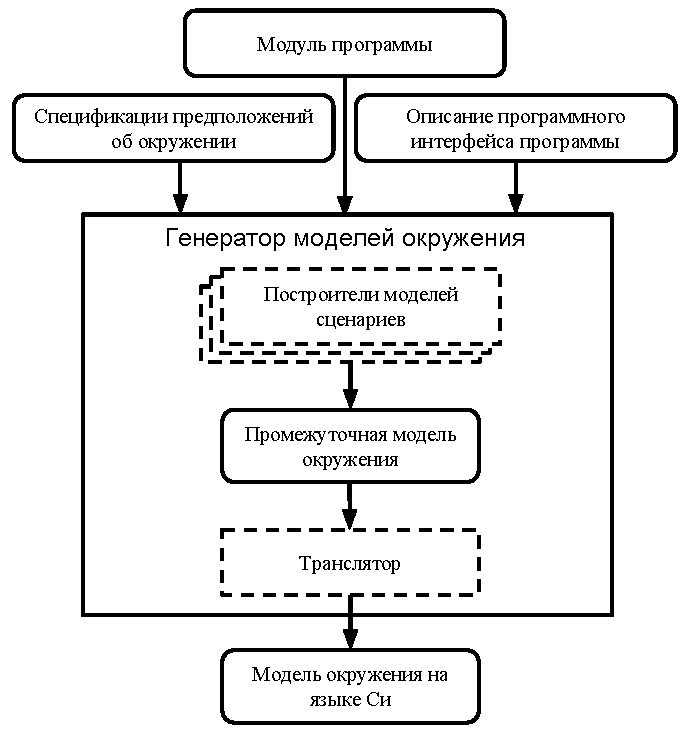
\includegraphics[scale=1.2]{generators}
\caption{Схема синтеза моделей окружения.}
\label{figure:em}
\end{figure}

Спецификации предположений об окружении содержат описания моделей сценариев взаимодействия на языке предметной области.
Построители выполняют подготовку моделей сценариев для промежуточной модели окружения на основе некоторого набора спецификаций предположений об окружении и описания программного интерфейса.
Предлагается использовать языки спецификации, расширяющие язык для задания промежуточной модели окружения, которым может быть либо язык Си расширениями для посылки и получения сигналов, либо специализированный язык предметной области.
Расширения должны учитывать особенности инструментов верификации, проверяемых требований, и верифицируемой программы.
Например, спецификация может представлять собой некоторый набор шаблонов моделей сценариев, на основе которых построитель может сгенерировать конкретные модели сценариев для промежуточной модели окружения. 
Для этого построитель определяет, какая часть программного интерфейса требует моделирования, определяя точки входа и неопределенные функции, а также другую необходимую информацию о программном интерфейсе.
Затем построитель использует те модели сценариев из спецификаций предположений об окружении, которые описывают вызов точек входа именно того модуля, для которого требуется подготовить модель окружения.

Предлагается использовать несколько построителей в зависимости от сложности и устройства верифицируемой программы.
Для крупных событийно-ориентированных программных систем на разработку построителей может требоваться значительное время.
Но универсальный алгоритм для данной задачи сформулировать трудно из-за широкого разнообразия программных систем и требований.

Рассмотрим пример работы простейшего построителя моделей сценариев для вызова функций по заданному пользователем списку имен.
Такой компонент выполняет следующие шаги:
\begin{enumerate}
    \item В качестве спецификации предположений об окружении пользователь передает список имен функций или шаблон, заданный при помощи регулярного выражения, и конфигурационные параметры, определяющие требуется ли вызывать функции в цикле.
    \item Построитель определяет на основе описания программного интерфейса конкретные функции, которые являются точками входа модуля программы и имена которых входят в список, заданный пользователем.
    Затем из описания программного интерфейса получаются сигнатуры точек входа.
    \item Для каждой функции выполняется генерация функции-обертки, помещаемой в тот файл, где определена точка входа. 
    Такая функция-обертка содержит инициализацию параметров с использованием вспомогательных функций для моделирования неопределенных значений, а также сам вызов целевой функции с данными параметрами.
    Обертка позволяет избежать ошибок, связанных с областью видимости типов, которые могут использоваться при задании сигнатуры аргументов точки входа, которую требуется вызвать.
    \item Построитель генерирует одну модель сценария для промежуточной модели окружения, которая вызывает точки входа. 
    Каждое действие модели сценария вызывает одну конкретную функцию-обертку.
    \item Отношение переходов, определяющее последовательность действий, зависит от конфигурационных параметров построителя.
    Если отношение переходов должно быть описано на языке программирования Си, тогда может использоваться оператор switch или цикл, в теле которого находится тот же оператор.
    Оператор switch в случайном порядке выполняет одно из действий --- вызов какой-либо функции-обертки.
    \item Все вспомогательные функции и модель сценария передаются транслятору.
\end{enumerate}

В некоторых случаях удобно вручную скорректировать или разработать модели сценариев для промежуточной модели окружения.
Такие модели сценариев необходимо иметь возможность передать в качестве входных данных генератору моделей окружения, чтобы они были добавлены в промежуточную модель для добавления к сгенерированным моделям сценариев, полученных построителями для определенных модулей, или для их замены.

Транслятор должен иметь ряд конфигурационных параметров, позволяющих настраивать вид модели окружения в зависимости от используемого инструмента верификации моделей программ или проверяемого требования.
На практике может возникать необходимость в следующих преобразованиях:
\begin{itemize}
    \item Выполнять трансляцию промежуточной модели окружения в последовательный или параллельный код на языке программирования Си. 
    При трансляции в последовательный код может требоваться подготовка модели окружения с разной степенью полноты с точки зрения всевозможных чередований событий из разных сценариев.
    \item Для задания параллельной модели окружения могут использоваться разные интерфейсы управления потоками или процессами.
    \item В модели окружения могут быть использованы разные наборы служебных функций.
\end{itemize}

В процессе своей работы транслятор выполняет следующие операции:
\begin{itemize}
    \item Объединяет полученные от построителей сценариев фрагменты промежуточной модели окружения на языке программирования Си, которые обозначались как $V_e, F_e, R_e, T_e$.
    \item Генерирует точку входа, которая вызывает служебную функцию инициализации модели требования.
    Затем в точке входа создаются потоки для сценариев, которые относятся к виду моделей потоков окружения.
    Для этого либо генерируется соответствующий код с созданием и ожиданием POSIX потоков, либо выполняется генерация последовательного кода с некоторым чередованием действий из разных сценариев.
    После завершения всех моделей сценариев в точке входа вызывается служебная функция завершения работы, определение которой находится в модели требования.
    \item Выполняет генерацию вспомогательного исходного кода для трансляции операций посылки и получения сигналов на язык программирования Си, например, в соответствие со схемой, предложенной при доказательстве теоремы об изоморфизме.
\end{itemize}

Модель окружения на языке программирования Си содержит набор файлов с исходным кодом, которые предлагается добавлять к модулю программы при помощи инструментации.
Данная операция выполняется на шаге компоновки верификационной задачи.

\section{Синтез моделей требований}

Для синтеза моделей требований предлагается использовать метод, предложенный ранее в работе~\cite{NovikovDis}.
Данный метод применялся в системе верификации LDV~Tools и показал возможность успешного применения на практике для проверки различных требований к драйверам операционной системы Linux~\cite{Zakharov2015, configurable:Trudy}.
Хотя в упомянутых работах метод применяется только для спецификации требований корректного использования интерфейса ядра в драйверах, он может быть использован и для других требований и программных систем.

Для формализации требования, согласно данному методу, требуется разработать контрактную спецификацию на аспектном расширении языка Си, называемую \textit{спецификацией требования}.
Спецификация содержит модели для функций и макрофункций программного интерфейса модулей программы, которые определены в окружении.
Спецификация позволяет свести задачу проверки требования к свойству корректности недостижимости ошибочного оператора.
Для некоторых требований, например, корректности работы с памятью, разрабатывать спецификацию нецелесообразно, так как модель требования будет чрезмерно сложной и вряд ли может быть проверена на практике инструментами верификации моделей программ.
В этом случае требование должно поддерживаться инструментом верификации в явном виде как проверка соответствующего свойства корректности.

Для генерации модели требования используется инструмент CIF для реализации подхода аспетно-ориентированного программирования, предложенного Е.~М.~Новиковым и апробированным при верификации драйверов ОС Linux в рамках системы верификации LDV~Tools~\cite{Novikov2013}.
Спецификация требования подается инструменту CIF вместе с исходным кодом модуля программы.
Инструмент выполняет препроцессирование исходного кода модуля и его инструментацию для синтеза модели требования на основе спецификации требования и добавления ее в исходный код модуля.

Спецификации предположений об окружении требований могут содержать определения одних и тех же функций.
Чтобы избежать конфликтов вводятся дополнительные служебные функции, которые определены в спецификации требования, но вызываются в модели окружения.
К таким служебным функциям относятся упомянутые ранее функции инициализации требования и функция завершения работы, которые соответствуют началу выполнения и завершению вызова точек входа модуля.
При вызове первой функции модель требования инициализирует начальное состояние,
а при вызове последней выполняет проверку условий, которые должны быть справедливы в момент завершения работы модуля или всех точек входа.
Например, при проверке требования корректной работы с некоторым счетчиком ссылок, модель требования инициализирует значение модели счетчика значением 0, а при вызове функции завершения работы проверяет, что все ссылки были успешно удалены и значение счетчика равно 0.

\section{Компоновка верификационных задач}
В качестве входных данных при компоновке верификационных задач выступают файлы с исходным кодом программы, файлы моделей окружения и требования, а также конфигурационные параметры, заданные пользователем.
В качестве результата компоновки из входных данных должна быть получена отдельная верификационная задача в формате, предложенном сообществом SV"~COMP.

Как ранее упоминалось, для получения исходного кода верификационной задачи может потребоваться инструментация исходного кода.
Для возможности применения данного метода модели должны быть сгенерированы в соответствующих форматах.
После или в процессе выполнения инструментации также следует препроцессировать исходный код всех файлов на языке программирования Си.
Некоторые инстрменты верификации моделей программ требуют, чтобы верификационная задача содержала только один файл.
В этом случае можно следует использовать инструменты для объединения файлов, например CIL~\cite{CIL}.

Для каждого требования следует подготовить соответствующую спецификацию свойства корректности и параметры в зависимости от инструмента верификации и его версии.
Комбинаций инструментов, версий и свойств корректности может быть достаточно много.
Поэтому может быть полезным ввести специальный формат с возможностью наследования наборов опций, чтобы сократить трудоемкость описания каждого набора конфигурационных параметров.

Последней частью верификационной задачи являются максимальные ограничения на вычислительные ресурсы: времени работы, процессорного времени, оперативной и дисковой памяти.
Набор ограничений позволяет также решать важную задачу воспроизводимости результатов.
Так как при использовании одной и той же аппаратуры важно иметь возможность воспроизвести результат и использовать полученные данные, например, для сравнения подходов к верификации или определения наиболее сложных для инструмента верификации верификационных задач с целью улучшить набор спецификаций.
% Глава 3 Архитектура
\chapter{Архитектура системы верификации}
В данной главе представлена архитектура системы верификации для синтеза и решения верификационных задач с использованием многоядерных и распределенных вычислительных систем.

\section{Компоненты системы верификации}
Подготовка и решение верификационных задач выполняются \textit{системой верификации}, для которой предлагается структура, представленная на рисунке~\ref{figure:system}. 
Система состоит из следующих компонентов:
\begin{itemize}
    \item сервер;
    \item решатель верификационных задач и заданий (далее решатель);
    \item генератор верификационных задач (далее генератор);
    \item инструменты верификации моделей программ.
\end{itemize}

\begin{figure}
\centering
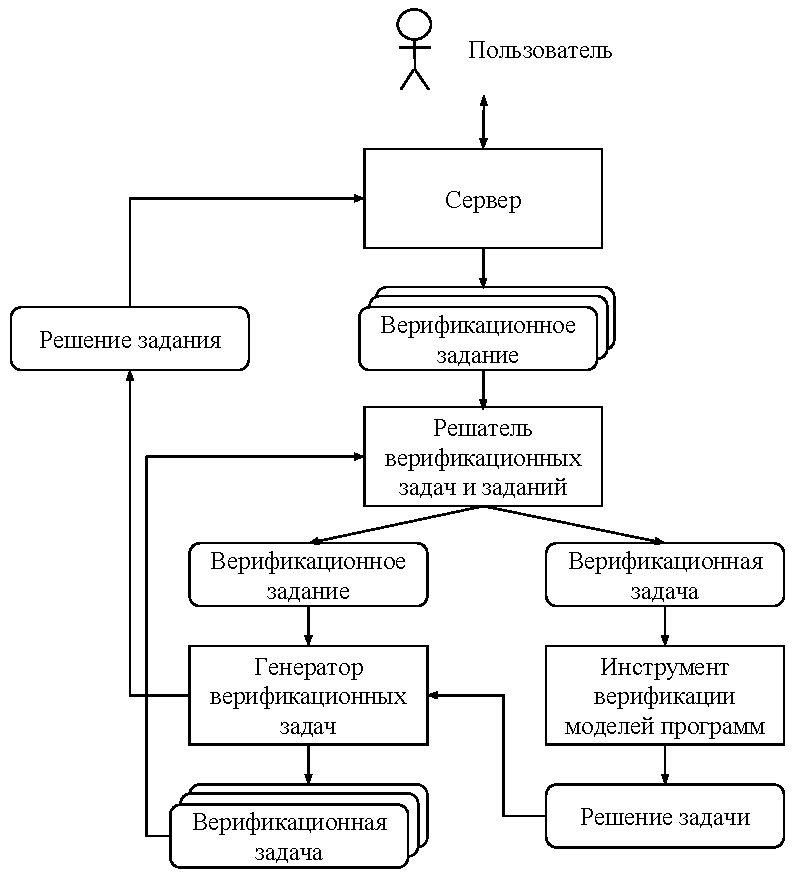
\includegraphics[scale=0.7]{system}
\caption{Структура системы верификации моделей программ.}
\label{figure:system}
\end{figure}

\section{Сервер}
Сервер выполняет следующие функции в рамках системы верификации:
\begin{itemize}
\item взаимодействие с пользователями;
\item организация взаимодействия между компонентами системы.
\item хранение результатов верификации; 
\end{itemize}

Пользователь взаимодействует с системой верификации через пользовательский интерфейс сервера.
Интерфейс предоставляет следующие функции:
\begin{itemize}
\item Позволяет создавать, изменять и удалять верификационные задания, которые содержат базу сборки программы, конфигурационные параметры и спецификации. 
Верификационное задание определяет ту часть программы, которая нуждается в проверке на соответствие заданным требованиям при определенных предположениях об окружении.
Верификационные задания могут включать десятки и сотни файлов, поэтому для каждой программы создается шаблон такого задания, а все последующие создаются пользователем при помощи его копирования и модификации.
\item Предоставляет возможность запуска и остановки решения верификационного задания, а также настройки ограничений на доступные при верификации вычислительные ресурсы. 
Пользователю должна быть доступна информация о всех решаемых верификационных заданиях, включая прогресс решения, оценку необходимого на завершение решения времени и полученные на текущий момент результаты.
Следует представлять пользователю информацию о статусе вычислительной системы, то есть объем доступных и используемых вычислительных ресурсов, подключенные узлы вычислительного кластера и их характеристики.
\item Реализует средства для экспертизы решений верификационных задач, включая оценку покрытия и предупреждений об ошибках.
\item Предоставляет инструменты для сравнения результатов решения верификационных заданий и переноса пользовательских оценок предупреждений об ошибках между результатами разными верификационных заданий, подготовленных для проверки требований к одной и той же программе.
\end{itemize}

В ходе работы между компонентами системы осуществляется активный обмен данными.
Верификационные задачи и задания между решателем и экземплярами генератора также передаются через сервер.
Данный компонент выполняет роль посредника между компонентами и надежного хранилища.
Такой подход позволяет избежать повторной передачи файлов, которые неоднократно могут отправляться компонентами.

В процессе верификации может накапливаться различная информация, которая может быть как получена автоматически в процессе верификации, так и подготовлена пользователем. 
Сервер предназначен для долговременного хранения полученных в ходе верификации артефактов в рамках верификационной системы.

\section{Генератор верификационных задач}
После того, как пользователь подготовил верификационное задание и инициировал его решение, оно попадает на вход решателю верификационных задач и заданий, который запускает экземпляр генератора верификационных задач.
Генератор выполняет подготовку верификационных задач согласно подходу, изложенному во второй главе. 
Кроме декомпозиции, синтеза моделей окружения и требований, композиции верификационной задач в формате, предложенном сообществом SV"~COMP, данный компонент выполняет дополнительные шаги: оценку прогресса решения верификационного задания, добавление атрибутов к верификационным задачам, отправку их решателю и ожидание результатов, первичную обработку решений верификационных задач и подготовку отчета о решении верификационного задания для его загрузки на сервер.

Атрибуты для верификационной задачи отражают ряд ее отличительных свойств, например, имя и версию программы, идентификатор проверяемого требования и т.п.
Атрибуты позволяют в пользовательском интерфейсе сравнивать результаты верификации, полученные в рамках различных верификационных заданий, и могут использоваться решателем при распределении вычислительных ресурсов.

Процесс подготовки верификационных задач может быть длительным, существенно превышающим время компиляции.
Поэтому подготовка задач должна выполняться параллельно и одновременно с их решением.
После декомпозиции программы на модули генератор верификационных задач выполняет шаги генерации верификационной задачи для каждого модуля независимо от остальных, поэтому этот процесс может быть естественным образом распареллелен.
Все генерируемые верификационные задачи отправляются затем решателю для запуска инструментов верификации моделей программ.

Результат решения каждой верификационной задачи состоит из вердикта, свидетельств нарушения или корректности, а также отчета о покрытии, который может быть подготовлен некоторыми инструментами верификации моделей программ.
Так как свидетельства нарушений об ошибках предназначены для валидации, а пользователю необходимо выполнять экспертизу сообщений об ошибках, то выполняется ряд преобразований свидетельств нарушений перед их отправкой на сервер:
\begin{itemize}
    \item Для каждой операции ошибочного пути в свидетельстве нарушения добавляется ссылка на модуль оригинального исходного кода программы, модели окружения или требования.
    Данное преобразование выполняется из-за того, что верификационная задача содержит препроцессированный, инструментированный срез исходного кода определенного модуля программы, который затруднительно анализировать пользователю.
    \item Помечаются операции ошибочного пути в зависимости от принадлежности оригинальному исходному коду программы или моделям окружения или требования.
    \item Добавляются аннотации на естественном языке для пользователя, чтобы объяснить модели событий сценариев взаимодействия в ошибочном пути, а также обосновать нарушение требования.
    \item Выделяются операции, либо релевантные проверяемому требованию, либо содержащие предположения инструмента верификации о неопределенных функциях, значениях переменных и памяти, которые могут оказаться неверными.
\end{itemize}

Покрытие выделяет ту часть программы, которая была проверена инструментом верификации моделей программ.
Хотя инструменты верификации проверяют все возможные пути выполнения в исходном коде верификационной задачи, неполная модель окружения, которая не содержит вызов определенных точек входа модуля, может привести к недостижимости некоторых фрагментов исходного кода.
Отчет о покрытии при верификации схож с отчетом о тестовом покрытии, но он может содержать и дополнительную информацию, например, предположения о диапазонах значений некоторых переменных, число состояний в модели программы для определенного участка верификационной задачи и т.д.
Следует выполнять аналогичные преобразования отчетов о покрытии, что были перечислены для свидетельств нарушений.
Отчеты о покрытии, полученные для разных верификационных задач для проверки одного и того же требования, могут быть объединены в единые итоговые отчеты.
Такой отчет передается генератором верификационных задач на сервер в составе отчета о завершении решения верификационного задания.

Решение верификационного задания может требовать много времени.
Например, система верификации LDV~Tools выполняет проверку драйверов одной версии ядра ОС Linux на соответствие одному требованию за время более суток, решая верификационные задачи последовательно.
Отправка результатов верификации во время решения верификационного задания параллельно с подготовкой и решением верификационных задач позволит на раннем этапе пользователю определить наличие ошибок в конфигурациях и спецификациях.

Обработку результатов решения верификационных задач также следует выполнять параллельно.
Решение каждой верификационной задачи не зависит от остальных, поэтому соответствующие отчеты о покрытии и свидетельства нарушений могут быть подготовлены независимо друг от друга и переданы на сервер.
Итоговые отчеты о покрытии и свидетельства нарушений после первичной обработки могут содержать файлы с исходным кодом программы, моделей требований и окружения.
Поэтому передача данных между сервером и экземплярами генератора верификационных задач должна минимизировать повторную передачу одних и тех же файлов, так как их число и размер могут быть достаточно велики.

\section{Решатель верификационных задач и заданий}
Верификационные задачи, подготовленные в процессе решения верификационного задания, поступают решателю для запуска необходимых инструментов верификации моделей программ.
Каждое верификационное задание и задача имеют максимальное ограничение на вычислительные ресурсы: объем доступных оперативной памяти и памяти на диске, время выполнения и процессорное время.
Ограничения необходимо соблюдать для получения воспроизводимых результатов верификации, поэтому, если инструмент верификации моделей программ или генератор верификационных задач превышают квоту выделенных им вычислительных ресурсов, они должны быть остановлены.
Для контроля за ограничениями потребления вычислительных ресурсов  предлагается использовать существующие решения, например, BenchExec~\cite{Beyer2016}.
Преимуществом применения BenchExec является наличие адаптеров для инструментов верификации моделей программ, делающих интеграцию и применение новых инструментов верификации менее трудоемкой.

Решатель верификационных задач и заданий предназначен для управления вычислительными ресурсами и планирования выполнения экземпляров других компонентов.
Задача управления вычислительными кластерами на сегодняшний день имеет множество решений и реализаций, пригодных для распараллеливания вычислительных задач разного вида, поэтому разрабатывать новый инструмент управления распределенной вычислительной системой избыточно.
В то же время облачные сервисы и системы управления вычислительными кластерами имеют разные функции и ограничения.
Например, в первой главе рассматривался облачный сервис Google App Engine, который позволяет распараллелить запуск инструментов верификации, но не позволяет задать необходимые для практического использования ограничения на вычислительные ресурсы.
Методы и инструменты выполнения облачных вычислений постоянно развиваются, поэтому система верификации не должна опираться в существенной степени на архитектуру какой-либо конкретной системы управления вычислительным кластером.
Поэтому предлагается реализовать отдельные модули в качестве адаптеров к той или иной системе распределенных вычислений в зависимости от ее функциональности:
\begin{itemize}
    \item модуль прогнозирования ограничения на максимальный объем оперативной памяти;
    \item модуль планирования для выбора вычислительного узла;    
    \item модуль запуска экземпляров инструментов верификации и генератора верификационных задач.
\end{itemize}

При решении верификационной задачи резервируется значительный объем оперативной памяти, чтобы соблюсти условие воспроизводимости результатов верификации.
На практике для верификации одного драйвера ОС Linux может требоваться резервирование порядка 10 ГБ оперативной памяти.
В то же время большая часть верификационных задач может требовать существенно меньшего объема вычислительных ресурсов, чем задано в максимальных ограничениях.
Модуль прогнозирования на основе статистики решения верификационных задач оценивает вероятное меньшее значение требуемой оперативной памяти для конкретной верификационной задачи.
Статистика решения верификационных задач собирается независимо для верификационных задач с определенными атрибутами.
При решении задачи подбора подходящего ограничения требуется минимизировать ошибку, иначе, если инструмент верификации потребует больше оперативной памяти, чем было задано в новом ограничении, верификационную задачу следует решать повторно уже с максимальным ограничением, что может занять десятки минут процессорного времени.

Модуль планирования либо выполняет распределение верификационных заданий и задач между узлами вычислительного кластера, либо передает их следующим модулям решателя в случае использования облачного сервиса с собственным планировщиком.
В случае самостоятельного планирования модуль решает следующую задачу: имеется некоторое количество узлов с определенными моделями процессоров, числом физических ядер, объемом оперативной и дисковой памяти; требуется разместить на вычислительных узлах для решения верификационные задачи и задания для минимизации общего времени решения верификационных заданий.
Всю оперативную память и физические ядра процессоров нельзя выделять для решения верификационных заданий, так как в этом случае может не остаться вычислительных ресурсов для решения верификационных задач, что приведет к бесконечному ожиданию запущенных экземпляров генератора.
Данная задача может быть решена при помощи простейшего жадного алгоритма, который будет гарантировать, чтобы для решения верификационных задач всегда оставалось доступно необходимое количество вычислительных ресурсов.
На практике могут быть реализованы различные алгоритмы, учитывающие разные аспекты планирования, например, приоритет решаемых верификационных заданий.

На последнем шаге модуль запуска либо отправляет верификационное задание или задачу в определенный облачный сервис, либо запускает необходимые экземпляры компонентов на заданном вычислительном узле с определенными ограничениями на вычислительные ресурсы.
Данный компонент должен поддерживать отмену решения верификационных заданий или задач, выполняя завершение всех дочерних процессов компонентов и сообщая модулю планирования об освобождении вычислительных ресурсов.
В случае ошибок журнал с их описанием должен быть отправлен на сервер для предупреждения пользователя.

% Глава 4 Реализация
\chapter{Реализация методов}
Предложенные в данной работе методы реализованы в системе верификации Klever для проверки требований к программным системам на языке программирования Си с расширениями GNU методом верификации моделей программ~\cite{klever}.
Klever является проектом с открытым исходным кодом, все компоненты которого реализованы на языке программирования Python 3.

Система Klever может быть установлена и использована на различных дистрибутивах операционной системы Linux и автоматически развернута и использована в облачной IaaS платформе OpenStack.

Для подготовки баз сборки используется инструмент Clade~\cite{clade}.
Clade выполняет контролируемую сборку программы на языке программирования Си для перехвата команд и извлечения необходимой информации о программном интерфейсе.
Для получения данных о файлах, функциях, глобальных переменных, типах и макросах используется механизм запросов к исходному коду, реализованный на основе упомянутого ранее инструмента CIF.

Структура верификационной системы соответствует архитектуре, предложенной в главе 3 данной работы.
Далее рассмотрена реализация отдельных компонентов системы верификации Klever.

\section{Сервер}
Сервер разработан на основе веб-фреймворка Django.
Для хранения компонент использует базу данных под управлением PostgreSQL.
Для установки пользователи могут использовать веб-серверы Apache2 с mod\_wsgi или NGINX с Gunicorn.

Пользовательский интерфейс сервера реализует все функции, необходимые для работы пользователей, которые были обозначены в третьей главе.
Работу с интерфейсом могут выполнять несколько пользователей с различными ролями, для которых настраиваются подходящие представления информации и права доступа.

Для анализа результатов пользователем реализованы представления ошибочных путей и отчетов о покрытии.
Разработаны вспомогательные промежуточные форматы, отличные от предложенных сообществом SV"~COMP, для добавления дополнительной информации к свидетельствам корректности и отчетам о покрытии в процессе первичной обработки результатов.
Интерфейс сервера позволяет сохранять подготовленные верификационные задачи в формате сообщества SV"~COMP для отладки инструментов верификации моделей программ и валидации результатов.

Для каждого свидетельства корректности или нарушения пользователь может указать экспертную оценку и отметить ряд атрибутов, добавленных генератором верификационных задач, по которым данное свидетельство может быть сопоставлено с другими при сравнении результатов решений верификационных заданий.
Атрибутами являются требование, имя проверяемой программы, ее версия и имя модуля.
При создании экспертной оценки пользователь отмечает, является ли вердикт решения верификационной задачи истинным или ложным и может оставить свой комментарий.
Экспертные оценки переносятся автоматически между верификационными задачами с одинаковыми значениями атрибутов.
Чтобы избежать ошибок при экспертизе из-за несовершенных алгоритмов переноса экспертных оценок и сравнения ошибочных путей, перенесенные оценки показываются в виде предложений пользователю с возможностью подтверждения или опровержения такой автоматической разметки результатов.

Для решаемых верификационных заданий оценивается прогресс решения на основе данных, периодически получаемых от генератора верификационных задач.
Оценка прогресса выполняется на основе подсчета числа решенных верификационных задач за равные интервалы времени и их общего числа.
Генератор верификационных задач в рамках каждого этапа своей работы периодически отправляет отчеты о ходе решения верификационного задания на сервер.
В зависимости от уровня отладки, состав отчетов может содержать различную информацию: журналы о выполнении компонентов, промежуточные данные, сообщения об ошибках, статистику о затраченных вычислительных ресурсах, отчеты о покрытии и свидетельства нарушения ошибок.
Вся полученная в данных отчетах информация становится сразу доступна пользователю для анализа и экспертизы.

Классификация ошибок и сбоев в инструментах верификации и компонентах генератора верификационных задач выполняется на основе \textit{описания проблем}.
Описание проблемы представляет собой идентификатор ошибки, описание ошибки на естественном языке и шаблон, заданный регулярным выражением, по которому ошибка обнаруживается в журнале выполнения компонента системы верификации.
При получении отчетов от генератора верификационных задач все журналы проверяются на предмет наличия проблем, описанных для соответствующих компонентов.
Система уже поставляется с набором описаний распространенных проблем, подготовленных заранее, что позволяет на раннем этапе диагностировать ошибки, допущенные пользователем при разработке спецификаций и конфигурировании системы верификации.

В процессе верификации моделей программ накапливаются различные данные, полученные автоматически системой верификации или подготовленные пользователями. 
К первому типу относятся свидетельства корректности и нарушений, база сборки, верификационные задачи, отчеты о покрытии, журналы выполнения компонентов и т.п.
Спецификации, экспертные оценки и описания проблем составляют данные, которые система верификации получает в процессе работы пользователя.
Некоторые результаты может требоваться хранить долгое время.
Поэтому сервер предлагает несколько режимов хранения результатов: полноценный и облегченный.
В полноценном режиме для каждого верификационного задания хранятся все артефакты, которые могут быть проанализированы пользователем.
После завершения работы пользователя с определенным верификационным заданием может быть включен облегченный режим хранения, в котором для данного задания удаляется большая часть данных, подготовленных автоматически системой верификации.

\section{Генератор верификационных задач}
Генератор верификационных задач начинает решение верификационного задания с получения конфигурационных параметров, базы сборки и спецификаций от сервера.
Затем выполняется проверка корректности и целостности полученных данных, включая разработанных пользователем спецификаций.
В случае, если все данные корректны запускаются следующие компоненты генератора:
\begin{itemize}
    \item компонент декомпозиции;
    \item компонент генерации верификационных задач;
    \item компонент обработки результатов;
    \item компонент обмена данными.
\end{itemize}

Затем выполняется декомпозиция программы на модули согласно методу, изложенному во второй главе.
Компонент выполняет шаги декомпозиции и предоставляет инфраструктуру для реализации различных стратегий выделения модулей и агрегации.
В рамках Klever уже реализованы стратегии выделения модулей для ядра ОС Linux и проекта BusyBox.

Для проверки требований к компонентам ядра ОС Linux была реализована стратегия выделения драйверов и подсистем.
Стратегия опирается на граф команд сборки и на основе специальных команд сборки для создания объекта ядра (англ. kernel object) драйвера, определяет входящие в его состав файлы на языке Си, а остальные файлы с исходным кодом из соответствующих директорий, компилируемые статически в ядро ОС, рассматриваются как подсистемы.
В результате стратегия выделяет модули, каждый из которых содержит исходный код либо драйвера, либо подсистемы.

Проект BusyBox объединяет несколько сотен пользовательских программ в виде одной программной системы.
Каждая программа называется апплетом (англ. applet).
Апплет состоит из нескольких файлов на языке программирования Си и опирается только на общую для проекта библиотеку функций libbb и стандартную библиотеку языка программирования Си.
Каждый апплет имеет строго одну точку входа, название которой строится как имя апплета и суффикс \textit{\_main}.
Сигнатура таких функций совпадает с сигнатурой функции \textit{main} пользовательских программ на языке программирования Си.
Стратегия для проекта BusyBox в качестве отдельных модулей выделяет библиотеку libbb и непосредственно апплеты.
В основе реализованной стратегии лежит алгоритм обхода графов файлов и функций для определения состава каждого апплета.

Для агрегации реализованы две стратегии на основе обхода графов функций и модулей с учетом отчетов о покрытии при верификации отдельных модулей.
Первая стратегия выполняет поиск в ширину модулей с определениями функций, отсутствующими в целевом модуле.
Вторая стратегия нацелена на поиск минимального набора модулей, который позволит вызвать как можно больше точек входа целевого модуля.
Отчеты о покрытии используются во второй стратегии для определения тех функций, вызывающих точки входа целевого модуля, которые достижимы при верификации с использованием некоторого набора спецификаций предположений об окружении.

Компонент генерации верификационных задач получает от компонента декомпозиции набор модулей и затем начинает параллельную подготовку для них моделей окружения и требований.
Процесс генерации отдельной верификационной задачи осуществляется набором плагинов, которые выполняют преобразования над исходным кодом модуля.
В конфигурации системы верификации для заданной программы пользователь выбирает те плагины, которые необходимы для подготовки соответствующих верификационных задач.
Первым плагином, как правило, запускается генератор моделей окружения, который в свою очередь содержит несколько построителей моделей сценариев и транслятор.

Для моделирования окружения драйверов и подсистем ядра ОС Linux разработаны два построителя: построитель моделей сценариев вызова обработчиков и построитель моделей сценариев вызова функций инициализации и выхода.
Генератор для вызова обработчиков требует от пользователя разработки спецификации предположений об окружении, описывающих сценарии вызова обработчиков определенных типов.
Формат спецификаций основан на формате задания промежуточной модели окружения, но содержит ряд дополнительных расширений.
Построитель моделей сценариев вызова функций инициализации и выхода требует для работы список макросов, при помощи которых можно определить функции инициализации и выхода драйверов и функции инициализации подсистем.
Набор таких макросов отличается от версии к версии ядра ОС Linux.
Модели сценариев, подготовленные построителем, выполняют вызов функций инициализации и выхода драйверов в соответствии с возможным порядком их загрузки и выгрузки операционной системой, который определяется при решении задачи топологической сортировки графа зависимостей между модулями.
Один из построителей моделей сценариев предназначен для вызова точек входа в произвольном порядке по списку имен функций или регулярному выражению, заданному пользователем.
Данный построитель может использоваться при верификации различных программ, включая апплеты BusyBox.

Транслятор генератора моделей окружения поддерживает подготовку параллельной модели окружения на языке программирования Си с использованием интерфейса управления потоками согласно стандарту POSIX.
Транслятор позволяет подготовить и последовательную модель окружения, но она является неполной из-за сокращения частичных порядков последовательностей событий разных моделей сценариев взаимодействия.
Практические эксперименты показали, что полная последовательная модель окружения, зачастую вызывает взрыв числа состояний в модели, построенной инструментом верификации, и ведет к ухудшению результатов верификации в целом.
Транслятор также позволяет использовать несколько разных наборов реализаций служебных функций для адаптации процесса синтеза моделей окружения для проверки разных требований и использования различных инструментов верификации моделей программ.

Для генерации моделей требований и компоновки исходного кода верификационных задач был реализован подход, апробированный в системе верификации LDV~Tools.
Необходимые компоненты были реализованы в виде плагинов.
Для инструментации и препроцессирования используется CIF, а для задания моделей окружения и требований соответствующее аспектно-ориентированное расширение языка Си.
CIF основан на GCC версии 7.1, поэтому инструмент поддерживает язык Си с расширениями GNU.
Компоновщик верификационных задач слайсера CIL из набора инструментов по дедуктивной верификации AstraVer Toolset~\cite{CILAstra}.
Формат генерируемых верификационных задач полностью следует формату SV"~COMP, поэтому в системе Klever могут применяться различные инструменты верификации.
Для задания конфигурационных параметров был предложен формат спецификаций, позволяющий описывать конфигурационные параметры для определенных версий и инструментов верификации в зависимости от проверяемого требования.

\section{Решатель верификационных задач и заданий}
Решатель верификационных задач и заданий предназначен для запуска экземпляров компонентов генератора верфикационных задач и инструментов верификации моделей программ.

Компонент осуществляет контроль за доступностью и потреблением вычислительных ресурсов и гарантирует изолированную работу данных компонентов.
Данная функциональность реализована при помощи BenchExec~\cite{Beyer2015}.

В рамках решателя были реализованы модуль прогнозирования ограничения на максимальный объем оперативной памяти, выполняющий расчет на основе ряда эвристических предположений и статистики измерения затраченных вычислительных ресурсов при решении верификационных задач.
Модуль планирования реализует жадный алгоритм выбора вычислительного узла для запуска экземпляров генератора верификационных задач и инструментов верификации с учетом приоритета верификационных заданий.
Основные модули запуска компонентов системы верификации позволяют решать верификационные задачи на одном вычислительном узле и в вычислительном кластере, управляемом при помощи VerifierCloud~\cite{VerifierCloud}.
Были также разработаны прототипы модулей запуска для использования систем управления вычислительным кластерами Docker Swarm~\cite{swarm} и Kubernetes~\cite{kubernetes}.

Для решения верификационных задач используются инструменты верификации моделей программ CPAchecker и Ultimate Automizer~\cite{Heizmann2015}.
Для интеграции других инструментов, поддерживающих формат верификационных задач сообщества SV"~COMP, требуется:
\begin{enumerate}
\item Описать конфигурационные параметры для требований, которые могут быть проверены при помощи данных инструментов.
\item Указать пути к исполняемым файлам инструментов в конфигурационных параметрах скриптов установки системы верификации Klever.
\end{enumerate}

На практике в системе верификации используются преимущественно различные версии инструмента верификации CPAchecker, в котором реализована выдача свидетельств нарушения и отчетов о покрытии в наиболее детальном виде.
Инструмент Ultimate Automizer, как и другие инструменты верификации сообщества SV"~COMP, позволяет получить результаты верификации, но из-за неполной информации об ошибочных путях анализ предупреждений об ошибках может быть трудным.


% Глава 5 Результаты
\chapter{Результаты практического применения}

В данной главе представлены результаты практического применения системы верификации Klever, разработанной на основе предложенных методов, и делаются выводы о пределах их применимости на практике.

\section{Критерии оценки результатов}
Процесс верификации крупных программных систем на языке программирования Си характеризуется показателями:
\begin{itemize}
    \item трудоемкостью получения результатов верификации;
    \item скоростью получения результатов верификации;
    \item точностью результатов верификации.
\end{itemize}

Предложенные в данной работе методы для верификации крупных программных систем на языке программирования Си нацелены прежде всего на сокращение трудоемкости и скорости верификации.
При этом необходимо показать, что точность верификации не ухудшилась.

Трудоемкость верификации зависит от трудозатрат, которые необходимы для конфигурирования и разработки спецификаций.
Скорость получения результатов определяется суммарным временем работы системы верификации, за которое выполняется генерация и решение верификационных задач.
Точность верификации будем рассматривать с точки зрения числа пропускаемых ошибок, числа предупреждений об ошибках и долей среди них истинных и ложных предупреждений, а также уровнем покрытия исходного кода при верификации.

Для оценки предложенных методов были рассмотрены результаты проверки требований к драйверам и подсистемам ядра ОС Linux~\cite{linux}, а также к апплетам проекта BusyBox~\cite{busybox}, которые представлены в следующих разделах данной главы. 

\section{Верификация ОС Linux}

В данном разделе рассматриваются результаты верификации драйверов и подсистем ОС Linux при помощи системы верификации Klever.
Все результаты получены для ядра ОС Linux в конфигурации allmodconfig для архитектуры x86\_64~\footnote{Система верификации Klever позволяет верифицировать исходный код и для других архитектур, но для этого требуется подготовка соответствующих инструментов, например, CIF.}.

Драйверы представляют собой событийно-ориентированные программы, которые загружаются в память ядра ОС динамически.
Подсистемами ядра ОС Linux называются компоненты ядра, которые статически компонуются в исполняемый файл ядра ОС Linux.
Подсистемы устройств реализуют поддержку для обработчиков драйверов определенных типов, например, TTY, Serial и других.
Драйверы, как правило, редко реализуют экспортируемые функции, а точками входа драйверов являются обработчики определенных типов.
Подсистемы ядра ОС Linux являются событийно-ориентированными программами и реализуют обработчики, как и драйверы.
Однако исходный код подсистем содержит достаточно экспортируемых функций, то есть выполняет роль библиотек.
Еще одним отличием подсистем от драйверов является другой интерфейс инициализации подсистем.
Подсистемы образуют иерархию, согласно которой ядро ОС вызывает функции инициализации подсистем в начале своей работы.

В ходе экспериментов рассматривались драйвера и подсистемы ОС Linux версии 3.14.79.
Для того, чтобы оценить трудоемкость для достижения высокого уровня точности, был выбран небольшой набор драйверов из директории drivers/serial.
Данная директория содержат 49 Serial драйверов с суммарным объемом исходного кода около 30 тысяч строк.
Для данного набора были разработаны спецификации предположений об окружении, чтобы модели окружения содержали вызов всех точек входа рассматриваемых драйверов.

Система позволяет выполнять проверку требований и для остальных драйверов ОС Linux.
Всего при декомпозиции было выделено 4371 модуль с исходным кодом драйверов.
Верификационные задачи были сгенерированы для 3864 модуля, суммарный размер исходного кода которых превышает три миллиона строк кода.
Для 405 модулей не была синтезирована модель окружения из-за отсутствия функций инициализации драйвера.
Такие драйверы экспортируют функции для других и для их верификации требуется разработка дополнительных спецификаций.
Еще 102 драйвера не были верифицированы из-за ошибок и ограничений в различных компонентах системы верификации Klever.

Для оценки применимости метода агрегации были выбраны три подсистемы ядра ОС Linux.
Информация о составе подсистем представлена в таблице~\ref{table:target_subsystems}.
Для более точной оценки результатов верификации число подсистем было ограничено из-за трудоемкости процесса верификации.

\begin{table}
\centering
\begin{tabular}{| l | l | c | c |}
\hline
Подсистема & Директория & Файлов & Строк кода \\
\hline
Character Devices Support (\textit{CHAR}) & drivers/char & 5 & 4194 \\ 
\hline
General-Purpose I/O (\textit{GPIO}) & drivers/gpio & 6 & 4472 \\ 
\hline
Terminal Devices Support (\textit{TTY}) & drivers/tty & 11 & 12129 \\ 
\hline
\end{tabular}
\caption{Исследуемые подсистемы ядра Linux 3.14.}
\label{table:target_subsystems}
\end{table}

\subsection{Трудоемкость верификации}
Самым трудоемким этапом процесса верификации является разработка спецификаций требований и предположений об окружении.
%Остальные этапы либо выполняются автоматически, либо требуют существенно меньше трудозатрат.
%На практике процесс верификации всегда проходит итеративно, но трудоемкость получения первичных результатов верификации в данной таблице не отражена.
Каждый драйвер реализует обработчики различных видов, для которых требуется разработать спецификации предположений об окружении, в которых должны быть заданы ограничения на порядок вызова обработчиков и их зависимости по данным.
Чтобы достичь уровня покрытия 100\% по функциям при верификации Serial драйверов, были разработаны различные спецификации предположений об окружении для нескольких построителей моделей сценариев.
Затем были разработаны дополнительные спецификации, чтобы достичь уровня покрытия около 50\% в среднем для всех драйверов ОС Linux.
В результате были разработаны спецификации для моделирования сценариев вызова обработчиков следующих типов: block, class, pci, hid, platform, serial, usb, а также для вызова обработчиков ethernet, file, ieee80211, net device, proto, real time clocks, scsi, sequential, block, tty, urb и моделирования механизмов отложенного выполнения таких, как таймеры, очереди, тасклеты, потоки ядра kthreads, а также для моделирования прерываний.
Спецификации были разработаны для версий ОС Linux 2.6.33, 3.14, 4.6.7, но самый полный и точный набор относится к версии 3.14.
%На начальных этапах апробации использовался подход вызова обработчиков на основе эвристик и для других типов обработчиков, чтобы увеличить покрытие исходного кода при верификации без необходимости разработки спецификаций.
%Но экспериментальные результаты показали, что число ложных срабатываний в таком случае существенно возрастает.

Всего для верификации драйверов ОС Linux было разработано в сумме около 17 тыс. строк кода спецификаций предположений об окружении на специализированном языке предметной области, основанном на предложенном в данной работе расширении языка Си.
Согласно оценкам, полученным на основе разработки спецификаций автором и студентами старших курсов вузов, трудоемкость разработки спецификации для одного типа обработчиков драйверов составляет 2 человеко-недели.
В этот процесс входит разработка спецификации, тестов и итеративное уточнение спецификации на основе полученных результатов верификации для исправления выявленных недостатков.

В качестве спецификаций требований использовались 30 спецификаций корректности использования интерфейсов ядра ОС Linux драйверами, разработанные для системы LDV~Tools.
Дополнительно были разработаны модели функций для проверки корректности работы с памятью и отсутствия гонок по данным, а также был реализован ряд служебных функций для связывания моделей требований и моделей окружения.
Таким образом, всего в системе верификации Klever имеется 32 спецификации требований для проверки драйверов и подсистем ОС Linux.
Трудоемкость разработки спецификаций требований оценивалась на основе тех показателей, которые были получены от разработчиков системы верификации LDV~Tools, так как задачи разработки новых спецификаций требований в данной работе на ставилось.

Оценка трудоемкости верификации Serial драйверов, всех драйверов и подсистем при помощи предложенного метода представлена в таблице~\ref{table:difficulty}.
В первом столбце представлены этапы работы, которые необходимо выполнить пользователю, за исключением времени анализа результатов, который в данной работе не рассматривается.
В ячейках представлена оценка трудоемкости и суммарный объем кода, разработанного на соответствующем этапе.
Оценка выполнялась в соответствии со следующей схемой:
\begin{enumerate}
    \item Первые результаты были получены для Serial драйверов, для которых приведены оценки трудоемкости и объем кода, который был разработан.
    \item При переходе к верификации остальных драйверов оцениваются дополнительные трудозатраты, которые были нужны после верификации Serial драйверов с учетом уже имеющихся стратегий, построителей и спецификаций.
    Второе число в каждой ячейке показывает новый суммарный объем исходного кода.
    \item При переходе к верификации подсистем новые спецификации не разрабатывались, чтобы подтвердить возможность повторного использования уже полученных артефактов.
    Поэтому соответствующие этапы содержат только трудозатраты на улучшение уточнение и доработку стратегий и спецификаций.
\end{enumerate}

Из-за высокой сложности драйверов ядра ОС Linux трудоемкость подготовки к верификации даже небольшого набора драйверов оказывается сопоставимой с трудоемкостью разработки спецификаций для верификации всех драйверов, объем исходного кода которых более чем в сто раз превосходит соответствующий объем кода Serial драйверов. 
С одной стороны, это демонстрирует масштабируемость метода и возможность его применения к крупным программным системам.
С другой стороны, применение системы верификации Klever для верификации небольшого числа отдельных компонентов крупной программной системы может быть достаточно трудным. 

%Трудозатраты для получения представленных результатов для подсистем составили  примерно один человеко-месяц.
%Основное время было потрачено на анализ результатов, доработку стратегии выделения модулей, исправление ошибок в спецификациях и доработку построителя моделей сценариев взаимодействия для поддержки вызова функций инициализации подсистем.
%Новые спецификации требований и предположений об окружении не разрабатывались, чтобы подтвердить возможность повторного использования имеющихся артефактов.

\begin{table}
\centering
\begin{tabular}{ | l | c | c | c |}
\hline
Этап разработки& Serial Драйверы & Все драйверы & Подсистемы\\
\hline
\shortstack[l]{Стратегий \\ декомпозиции} & 
\shortstack[c]{0,25 чел. мес. \\ 100LOC Python} & 
\shortstack[c]{0 чел. мес. \\ 100LOC Python} &
\shortstack[c]{0,25 чел. мес. \\ 120LOC Python} \\
\hline
\shortstack[l]{Построителей \\ моделей сценариев} & 
\shortstack[c]{3 чел*мес \\ 3KLOC Python} &
\shortstack[c]{0 чел*мес \\ 3KLOC Python} &
\shortstack[c]{0,5 чел*мес \\ 3,5KLOC Python} \\
\hline
\shortstack[l]{Спецификаций \\ предположений \\об окружении} & 
\shortstack[c]{4,5 чел*мес \\ 7KLOC DSL} &
\shortstack[c]{5,5 чел*мес \\ 17KLOC DSL} &
\shortstack[c]{0 чел*мес \\ 17KLOC DSL} \\
\hline
\shortstack[l]{Спецификаций \\ требований} &
\shortstack[c]{6 чел*мес \\ 550LOC DSL} &
\shortstack[c]{9 чел*мес \\ 1500LOC DSL} & 
\shortstack[c]{0,25 чел*мес \\ 1500LOC DSL} \\
\hline
\textbf{Итого} & 13,75 чел*мес & 14,5 чел*мес & 1 чел*мес \\
\hline
\end{tabular}
\caption{Трудоемкость верификации драйверов и подсистем ОС Linux.}
\label{table:difficulty}
\end{table}

\subsection{Скорость верификации}
Для измерения скорости верификации использовались вычислительные машины с процессорами Intel Core i7-7700 CPU @ 3.60GHz с 4 физическими ядрами.
На решение каждой верификационной задачи отводилось 15 ГБ оперативной памяти и 900 секунд.
Для верификации использовался инструмент CPAchecker версии 1.7.

В таблице~\ref{table:speed} приведены результаты верификации драйверов ОС Linux версии 3.14.79.
При верификации проверялись наборы из 49 Serial драйверов и 3864 всех драйверов на соответствие 30 требованиям корректности использования интерфейса ядра в драйверах.
В первой таблице приведены результаты, в рамках которых генератор верификационных задач выполнял подготовку задач последовательно, а решатель не запускал экземпляры инструментов верификации параллельно.
В следующем столбце представлены результаты, когда ограничения на использование физических ядер не устанавливались, а для решения использовалась одна вычислительная машина.
В последнем столбце представлен результат при использовании 30 вычислительных машин.
Время верификации Serial драйверов не может быть меньше времени подготовки верификационных задач, которое составляет 30 минут при использовании 4 физических ядер.
При верификации всех драйверов время удается существенно сократить, так как в этом случае на работу инструмента верификации тратится гораздо больше времени по сравнению с временем подготовки верификационных задач.

\begin{table}
\centering
\begin{tabular}{| l | c | c | c |}
\hline
Верификационное задание & 2 физ. ядра & 4 физ. ядра & 30 * 4 физ. ядра \\
\hline 
Serial драйверы (30KLOC) & 5ч & 2,7ч & 0,5ч \\
\hline 
Все драйверы (3MLOC) & 600ч & 195ч & 11ч \\
\hline
\end{tabular}
\caption{Время верификации драйверов ОС Linux версии 3.14.79.}
\label{table:speed}
\end{table}

\subsection{Точность верификации}

Таблица \ref{table:coverage} представляет покрытие исходного кода драйверов из директорий drivers ядра ОС Linux версии 3.14.79 и некоторых других директорий, содержащих драйверы, приведенных для сравнения.
В таблице \ref{table:drivers} представлены результаты оценки покрытия драйверов из директорий, вложенных в директорию drivers.
В среднем покрытие драйверов из директории drivers составило 51\% по строкам и 45\% по функциям.
Такой уровень покрытия уже позволяет обнаруживать ошибки в драйверах, которых при помощи системы верификации Klever было выявлено около сотни.

Уровень покрытия исходного кода зависит от числа вызываемых в моделях окружения обработчиков.
На рисунке \ref{figure:handlers} представлена зависимость доли реализаций обработчиков драйверов наиболее популярных типов относительно числа реализаций обработчиков всех типов для ОС Linux 3.14.79. Из графика видно, что более 80\% всех обработчиков имеют тип из числа 100 наиболее популярных.
Таким образом, чтобы получить значительно больший уровень покрытия по исходному коду, потребуется затратить существенно больше усилий на разработку спецификаций предположений об окружении для поддержки новых типов обработчиков драйверов.

\begin{figure}
\centering
\begin{tikzpicture}
\begin{axis}[
    xlabel={Число типов обработчиков},
    ylabel={Доля реализаций обработчиков},
    xmin=0, xmax=700,
    ymin=0, ymax=100,
    xtick={0,100,200,300,400,500,600,700},
    ytick={0,20,40,60,80,100},
    yticklabel={\pgfmathprintnumber\tick\%}
]
\addplot coordinates {(1,15) (2,27) (3,40) (4,45) (5,48) (10,60) (20,71) (50,82) (100,88) (200,94) (300, 96) (500, 99) (700, 100)};
\end{axis}
\end{tikzpicture}
\caption{Зависимость доли реализаций обработчиков наиболее распространенных типов от числа всех обработчиков драйверов ОС Linux 3.14.}
\label{figure:handlers}
\end{figure}

\begin{table}
\centering
\begin{tabular}{ | l | l | l |}
\hline
Директория & Покрытие по строкам & Покрытие по функциям\\
\hline
arch & 46\% (3340/7222) & 21\% (103/486)\\
\hline
block & 14\% (429/2955) & 1\% (4/267)\\
\hline
crypto & 39\% (7411/18793) & 23\% (168/722)\\
\hline
drivers & 55\% (1398511/2538372) &  45\% (49820/110525) \\
\hline
net & 28\% (72746/254327) & 26\% (3455/13180) \\  	
\hline
fs & 25\% (69221/267952) & 17\% (2051/11736) \\ 	
\hline
sound & 57\% (151810/262443)  & 29\% (3029/10419) \\ 
\hline
\end{tabular}
\caption{Уровень покрытия исходного кода загружаемых модулей из различных директорий ядра ОС Linux 3.14.79.}
\label{table:coverage}
\end{table}

\begin{table}
\centering
\begin{tabular}{| l | l | l |}
\hline
Директория & Покрытие по строкам & Покрытие по функциям\\
\hline 
drivers/gpu & 13\% (13476/96446)  & 4\% (190/4626) \\  	
\hline
drivers/infiniband & 34\% (36314/104686) &  24\% (1056/4357) \\
\hline
drivers/isdn & 58\% (30777/52354) 	& 52\% (993/1877) \\
\hline
drivers/media &  47\% (118324/249319) & 27\% (2687/9677) \\
\hline
drivers/net & 66\% (363300/549366) & 62\% (15033/24147) \\
\hline
drivers/staging & 66\% (161825/244187) & 55\% (4554/8250) \\
\hline
drivers/usb & 57\% (96389/168336)  & 53\% (3796/7101) \\
\hline
drivers/video & 58\% (32225/54924) & 48\% (1127/2302) \\  
\hline
\end{tabular}
\caption{Уровень покрытия исходного кода драйверов из директории ядра ОС Linux 3.14.78.}
\label{table:drivers}
\end{table}

Serial драйверы проверялись на соответствие всем 32 требованиям.
Система верификации LDV~Tools позволяет проверять 30 правил корректности использования интерфейса ядра в драйверах из данного набора.
Но уровень точности моделей окружения в LDV~Tools не позволял выполнять проверку требований корректности работы с памятью и отсутствия гонок по данным.
Для того, чтобы оценить точность моделей окружения в сравнении с подходом, реализованным в системе верификации LDV~Tools, для выбранных драйверов были выполнены соответствующие эксперименты, результаты которых представлены в таблице~\ref{table:serialldv}.
В первой строке таблицы приведены результаты верификации Serial драйверов при помощи системы верификации Klever на соответствие всем требованиям.
Во второй строке представлены результаты верификации, полученные при помощи системы верификации Klever, только для тех требований, проверка которых может быть выполнена и при помощи системы верификации LDV~Tools.
Третья строка содержит результаты, полученные при помощи системы верификации LDV Tools.
Предупреждения, выданные в рамках системы верификации LDV~Tools, содержат существенно больше ложных предупреждений об ошибках из-за некорректных моделей окружения, которые в рамках этой системы верификации исправить не представляется возможным.
%Данный результат подтверждает, что точность моделей окружения в системе верификации Klever повысилась.

Проверка требований корректности работы с памятью и отсутствия гонок по данным стала возможной в системе верификации Klever с появлением конфигурируемого транслятора промежуточной модели окружения, который позволяет настраивать вид моделей окружения в зависимости от проверяемого требования к программе.
Новые обнаруженные ошибки демонстрируют важность данной функции на практике.

\begin{table}
\centering
\begin{tabular}{| l | c | c | c | c |}
\hline
\shortstack[l]{Верификационное \\ задание} &
\shortstack[l]{Ложное \\ предупреждение} &
Ошибка & Нет вердикта\\
\hline
\shortstack[l]{Klever, Serial \\ драйверы, расширенный \\ набор требований} & 16  & 6 & 46\\ 
\hline
\shortstack[l]{Klever, Serial \\ драйверы, сокращенный \\ набор требований} & 5  & 1 & 16\\ 
\hline
\shortstack[l]{LDV Tools, Serial \\ драйверы, сокращенный \\ набор требований} & 31  & 0 & 9\\
\hline
\end{tabular}
\caption{Вердикты при верификации Serial драйверов ОС Linux версии 3.14.79.}
\label{table:serialldv}
\end{table}

Эксперименты с подсистемами ядра ОС Linux выполнялись для исследования возможности повторного использования спецификаций при верификации, поэтому при верификации подсистем новые спецификации не разрабатывались.
Чтобы повысить уровень покрытия при верификации был использован подход агрегации подсистем с драйверами.

Чтобы выяснить, как на точность результатов влияет верификация разных версий ядра ОС с одним и тем же набором спецификаций требований и предположений об окружении, были рассмотрены версии ядра ОС Linux, начиная с 3.9, выпущенной 28 апреля 2013, и заканчивая 3.19, выпущенной 8 февраля 2015.
За рассматриваемый почти 2-х летний период разработки было выпущено 11 версий ядра.
Таблица \ref{table:target_subsystem_changes} отражает число изменений, сделанных в подсистемах за данный период.

\begin{table}
\caption{Изменения в исходном коде целевых подсистем относительно версии ОС Linux 3.14}
\label{table:target_subsystem_changes}
\centering
\begin{tabular}{ l l l }
\hline
Подсистема & Файлов добавлено/удалено & Строк добавлено/удалено\\
\hline
\textit{CHAR} & +0/-1 (+0\%/-20\%) & +950/-712 (+23\%/-17\%) \\ 
\textit{GPIO} & +2/-3 (+33\%/-50\%) & +5074/-3079 (+113\%/-69\%) \\ 
\textit{TTY} & +1/-0 (+9\%/-0\%) & +4012/-3221 (+33\%/-27\%) \\ 
\hline
\end{tabular}
\end{table}


\begin{figure}
\centering
\begin{tikzpicture}
\begin{axis}[
  width=13cm,
  height=7cm,
  grid=major,
  xlabel=Версия ядра Linux,
  ylabel=Покрытие по функциям,
  xtick=data,
  xticklabels={3.9,3.10,3.11,3.12,3.13,3.14,3.15,3.16,3.17,3.18,3.19},
  yticklabel={\pgfmathprintnumber\tick\%},
  ymin=40,
  ymax=100,
  legend style={
    at={(0.95,0.5)},
    anchor=west
  }
]
\addplot coordinates {(0,77.2) (1,78.8) (2,78.6) (3,78.6) (4,77.6) (5,77.6)	(6,76.2) (7,76.2) (8,74.0) (9,73.8)	(10,73.8)};
\addlegendentry{CHAR}
\addplot coordinates {(0,53.0) (1,51.8) (2,54.2) (3,54.7) (4,49.7) (5,59.1)	(6,53.5) (7,59.6) (8,63.6) (9,64.3)	(10,54.2)};
\addlegendentry{GPIO}
\addplot coordinates {(0,81.2) (1,80.7) (2,76.5) (3,82.9) (4,82.9) (5,83.0)	(6,82.5) (7,82.5) (8,82.5) (9,82.7)	(10,83.0)};
\addlegendentry{TTY}
\end{axis}
\end{tikzpicture}
\caption{Уровень покрытия по функциям исходного кода целевых подсистем.}
\label{figure:func_coverage}
\end{figure}

График на рисунке~\ref{figure:func_coverage} отражает покрытие по функциям в зависимости от версии ядра ОС Linux.
Покрытие подсистем CHAR и TTY меняется незначительно.
В подсистеме TTY в версии 3.11 был добавлен новый файл с определениями семафоров, которые на тот момент еще не использовались в других файлах подсистемы или драйверов, что вызвало падение покрытия при верификации.
Покрытие по функциям подсистемы GPIO меняется значительно из-за активной разработки подсистемы в рассматриваемый период.
Подсистема была добавлена в 2008~\cite{gpio} и достаточно активно менялась в отличие от CHAR и TTY еще долгое время.
Насколько значительно изменялись подсистемы относительно версии ядра ОС Linux 3.14 можно видеть из таблицы \ref{table:target_subsystem_changes}.

\begin{figure}
\centering
% \subfigure[Total statistics]{
% \begin{tikzpicture}
% \pie[radius=2, scale font, text=legend, sum=auto]{
%   105/Absent environment model specifications,
%   40/Invoked from other subsystems,
%   10/Replaced with models,
%   10/No invocations at all,
%   9/Another architecture and configuration
% }
% \end{tikzpicture}
% }
% \subfigure[Statistics for each subsystem]{
\begin{tikzpicture} \begin{axis}[ 
  ybar,
  enlargelimits=0.25,
  legend style={
    at={(0.8,0.75)},
    anchor=west
  },
  ylabel=Непокрытие функции,
  symbolic x coords={CHAR,GPIO,TTY},
  xtick=data,
  nodes near coords,
  nodes near coords align={vertical}
]
\addplot coordinates {(CHAR,14) (GPIO,46) (TTY,45)};
\addplot coordinates {(CHAR,9) (GPIO,15) (TTY,16)};
\addplot coordinates {(CHAR,2) (GPIO,0) (TTY,8)};
\addplot coordinates {(CHAR,1) (GPIO,5) (TTY,4)};
\addplot coordinates {(CHAR,0) (GPIO,5) (TTY,4)};
\legend{Нет спецификаций,Вызов из другой подсистемы,Функция заменена моделью,Функция не вызывается,Другая архитектура/конфигурация}
\end{axis}
\end{tikzpicture}
% }
\caption{Причины отсутствия покрытия функций для исследуемых подсистем из ядра ОС Linux версии 3.14.}
\label{figure:func_no_coverage}
\end{figure}

На диаграмме на рисунке \ref{figure:func_no_coverage} отражены причины отсутствия покрытия по функциям.
Для вызова некоторых обработчиков требовалась разработка спецификаций предположений об окружении.
Некоторые функции, которые вызывались только из другой подсистемы, требовали добавления в состав агрегаций еще и других подсистем, а не только драйверов, но этот подход не был реализован.
Некоторые функции вовсе не имели вызовов в рассматриваемых версиях ядра.
Ряд функций вызывался только в исходном коде, предназначенном для другой архитектуры или конфигурации ядра.

\begin{figure}
\centering
\begin{tikzpicture}
\begin{axis}[
  width=13cm,
  height=7cm,
  grid=major,
  xlabel=Версия ядра Linux,
  ylabel=Среднее число вердиктов,
  xtick=data,
  xticklabels={3.9,3.10,3.11,3.12,3.13,3.14,3.15,3.16,3.17,3.18,3.19},
  legend style={
    at={(0.95,0.5)},
    anchor=west
  }
]
\addplot[blue,mark=*]         coordinates {(0,9.0) (1,9.0) (2,9.0) (3,9.0) (4,9.0) (5,9.0) (6,9.0) (7,9.0) (8,9.0) (9,9.0) (10,9.0)};
\addlegendentry{CHAR True}
\addplot[red,mark=*]          coordinates {(0,9.0) (1,8.1) (2,8.8) (3,8.6) (4,8.6) (5,8.7) (6,8.8) (7,9.8) (8,8.8) (9,8.8) (10,10.2)};
\addlegendentry{GPIO True}
\addplot[brown,mark=*]        coordinates {(0,7.4) (1,7.4) (2,7.4) (3,7.4) (4,7.4) (5,7.4) (6,7.4) (7,7.4) (8,7.4) (9,7.5) (10,7.5)};
\addlegendentry{TTY True}
\addplot[blue,mark=square*]   coordinates {(0,0.0) (1,0.0) (2,0.0) (3,0.0) (4,0.0) (5,0.0) (6,0.0) (7,0.0) (8,0.0) (9,0.0) (10,0.0)};
\addlegendentry{CHAR False}
\addplot[red,mark=square*]    coordinates {(0,0.5) (1,0.5) (2,0.5) (3,0.5) (4,0.5) (5,0.6) (6,0.9) (7,0.8) (8,1.8) (9,1.7) (10,0.5)};
\addlegendentry{GPIO False}
\addplot[brown,mark=square*]  coordinates {(0,0.6) (1,0.3) (2,0.3) (3,0.7) (4,0.8) (5,0.7) (6,0.7) (7,0.7) (8,0.7) (9,0.6) (10,0.3)};
\addlegendentry{TTY False}
\addplot[blue,mark=diamond*]  coordinates {(0,3.0) (1,3.0) (2,3.0) (3,3.0) (4,3.0) (5,3.0) (6,3.0) (7,3.0) (8,3.0) (9,3.0) (10,3.0)};
\addlegendentry{CHAR Unknown}
\addplot[red,mark=diamond*]   coordinates {(0,2.5) (1,3.4) (2,2.8) (3,2.9) (4,2.9) (5,2.7) (6,2.3) (7,1.4) (8,1.5) (9,1.5) (10,1.2)};
\addlegendentry{GPIO Unknown}
\addplot[brown,mark=diamond*] coordinates {(0,4.0) (1,4.3) (2,4.3) (3,3.9) (4,3.8) (5,3.9) (6,3.9) (7,3.9) (8,3.9) (9,3.9) (10,4.2)};
\addlegendentry{TTY Unknown}
\end{axis}
\end{tikzpicture}
\caption{Среднее число вердиктов при верификации целевых подсистем в зависимости от версии ОС Linux.}
\label{figure:verdicts}
\end{figure}

Целевые подсистемы были верифицированы на соответствие 12 релевантным требованиям: memory, alloc:\{irq, spinlock\}, arch:io, base:\{class, dma-mapping\}, fs:sysfs, locking:\{mutex, rwlock, spinlock\}, kernel:module, rcu:update:lock.
На рисунке~\ref{figure:verdicts} представлено изменение результатов верификации в зависимости от версии ядра.
Среднее число вердиктов позволяет на одном графике сравнить результаты для всех трех подсистем. 
Причины изменений можно видеть из графиков с покрытием функций в зависимости от версии ядра ОС Linux~\ref{figure:func_coverage}.
Например, в версии Linux 3.17 и Linux 3.18 была внесена ошибка, которая обнаруживалась Klever при проверке требования locking:spinlock.

В подсистемах CHAR и TTY не было найдено ошибок.
При верификации подсистемы TTY 62\% ложных сообщений об ошибках относились к подсистеме, а остальные 38\% относились к драйверам, с которыми проверялась подсистема.
Все ложные сообщения были вызваны неточностью спецификаций предположений об окружении.
В подсистеме GPIO 51\% всех вердиктов False являются подтвержденными ошибками.
Одна из ошибок уже упомянута и была внесена в исходный код ОС Linux в версии 3.17 и исправлена в версии 3.19.
Еще 2 ошибки были найдены в драйверах и не были исправлены в новых версиях ядра.
Для подсистемы GPIO 59\% ложных сообщений об ошибках относились к исходному коду подсистемы и 41\% к драйверам.
Причиной 86\% ложных сообщений об ошибках являются неточные спецификации предположений об окружении, а 14\% вызваны неточностью инструмента верификации CPAchecker.

% CHAR: 77
% GPIO: 130
% TTY: 281
Также для выбранных версий ядра была попытка обнаружить ошибки, исправленные в рассматриваемый период и которые нарушают требования, проверку которых можно осуществить при помощи системы верификации Klever.
Для этого были проанализированы вручную 488 изменений, исключая слияния веток, сделанные начиная с версии 3.9 и заканчивая 3.19 в репозитории ОС Linux~\cite{linuxrepo}.
Среди найденных исправлений ошибок были найдены 8 подходящих, представленные в таблице~\ref{table:target_subsystem_faults}.

\begin{table}
\centering
\begin{tabular}{ c l l l }
\hline
Название & Изменение & Требование & Статус \\
\hline
\multirow{3}{*}{\textit{CHAR}} & 08d2d00b291e & \textit{memory} & \ding{55} (Иная конфигурация) \\ 
                               & b5325a02aa84 & \textit{memory} & \ding{51}  \\ 
                               & 61c6375d5523 & \textit{memory} & \ding{55} (Иная конфигурация) \\ 
\hline
\multirow{2}{*}{\textit{GPIO}} & e9595f84a627 & \textit{memory} & \ding{51} \\ 
                               & 00acc3dc2480 & \textit{locking:spinlock} & \ding{51} \\ 
\hline
\multirow{3}{*}{\textit{TTY}}  & b216df538481 & \textit{memory} & \ding{55} (Ограничение инструмента) \\ 
                               & 07584d4a356e & \textit{kernel:module} & \ding{51}  \\ 
                               & 1d9e689c934b & \textit{memory} & \ding{55} (Не хватило ресурсов) \\  
\hline
\end{tabular}
\caption{Результат поиска известных ошибок в рассматриваемых подсистемах.}
\label{table:target_subsystem_faults}
\end{table}

Ошибка из изменения \textit{00acc3dc2480} была уже упомянута и была успешно обнаружена Klever.
Для поиска ошибок из \textit{b5325a02aa84} и \textit{e9595f84a627} потребовалось добавить больше драйверов в агрегации, с которыми верифицировалась подсистема из-за нехватки моделей некоторых неопределенных функций.
Ошибка \textit{07584d4a356e} как таковая не была обнаружена, но инструмент доказал недостижимость данного исходного кода из-за другой ошибки в подсистеме.

Чтобы обнаружить ошибку, исправленную в \textit{08d2d00b291e}, требовалось анализировать исходный код подсистемы \textit{CHAR} для архитектуры \textit{x86\_32}.
Для обнаружения ошибки, исправленной в \textit{61c6375d5523}, необходимо было использовать конфигурацию, отличную от \textit{allmodconfig}.
Чтобы найти ошибку до исправления \textit{b216df538481} требовался более точный анализ вызовов по функциональным указателям, который не был реализован в соответствующей версии CPAchecker на момент выполнения экспериментов.
Из-за недостаточной масштабируемости данного инструмента верификации моделей программ также не удалось обнаружить ошибку, исправленную в \textit{1d9e689c934b}.

\section{Верификация апплетов проекта BusyBox}
В отличие от драйверов и подсистем ОС Linux проект BusyBox содержит пользовательские программы, которые имеют одну точку входа и являются преобразующими с точки зрения устройства.
Чтобы продемонстрировать возможность применения системы верификации Klever и к таким программных системам, были выполнены соответствующие эксперименты.
В данном разделе представлены результаты верификации проекта BusyBox версии 1.28.3 в конфигурации alldefconfig для архитектуры x86\_64.

\subsection{Трудоемкость верификации}
Подготовка к верификации апплетов BusyBox состояла из следующих этапов:
\begin{itemize}
    \item разработка стратегии выделения модулей и спецификации декомпозиции;
    \item разработка спецификаций предположений об окружении с моделями функций стандартной библиотеки;
    \item разработка спецификаций требований.
\end{itemize}
Так как каждый апплет имеет одну точку входа, то разработка спецификаций для моделирования сценариев не потребовалась, поэтому был использован построитель моделей сценариев, который выполняет подготовку промежуточной модели окружения полностью автоматически.
Суммарное время выполнения данных этапов составило около одного человеко-месяца и представлено в таблице~\ref{busybox:difficulty}.

Для проверки требований были разработаны две спецификации.
Проверка требования корректности работы с файловыми дескрипторами была сведена к проверке свойства недостижимости ошибочного оператора, а для проверки требования корректности работы с памятью потребовалось разработать ряд моделей функций стандартной библиотеки. 
Для сокращения числа ложных предупреждений об ошибках были разработаны 34 модели различных функций.

\subsection{Скорость верификации}
Для верификации использовалась 8-ядерная виртуальная машина, работающая на процессорах \mbox{Intel Xeon E312xx} (Sandy~Bridge) CPU, с 64~Гб оперативной памяти.
Для решения верификационных задач был использован инструмент верификации моделей программ CPAchecker.
На решение каждой верификационной задачи отводилось 15 Гб оперативной памяти и 900 секунд процессорного времени.

Время верификации составило 5,5 и 7 часов при проверке корректности работы с памятью и корректности использования файловых дескрипторов соответственно.
По сравнению с верификацией драйверов ОС Linux заметно существенно снижение скорости работы инструмента верификации при верификации апплетов, что было вызвано невозможностью использования слайсера при подготовке верификационных задач.

\subsection{Точность верификации}
При верификации апплеты проверялись на соответствие требованиям корректности работы с файловыми дескрипторами и памятью.
Уровень покрытия при верификации составил 97\% по строкам и 94\% по функциям.

При проверке требования корректности работы с памятью приемлемого уровня точности достигнуть не удалось.
Основным ограничением в данном случае стала недостаточная точность моделирования операций со строками в инструменте верификации моделей программ CPAchecker.

Результаты проверки требования корректности работы с файловыми дескрипторами приведены в таблице~\ref{table:busy}.
Нарушение проверяемого требования апплетом ssl\_client отмечено как истинное предупреждение, так как апплет требует в качестве входных данных передачи уже открытых файловых дескрипторов, что было запрещено формальной моделью требования.
Одна ложная ошибка была вызвана неточной моделью аргументов командной строки апплета, а в остальных 5 случаях причиной стала недостаточная точностью инструмента верификации при моделировании операций с массивами, функциональными указателями и битовыми векторами.
Для 105 апплетов вердикт не удалось получить за приемлемое время из-за проблемы взрыва числа состояний в модели. 
Еще 23 апплета не были проверены из-за ошибок в инструменте CIF.

\begin{table}
\centering
\begin{tabular}{ | l | c | c | c |}
\hline
Этап разработки& BusyBox\\
\hline
\shortstack[l]{Стратегий \\ декомпозиции} & 
\shortstack[c]{0,25 чел. мес. \\ 100LOC Python} \\ 
\hline
\shortstack[l]{Построителей \\ моделей сценариев} & 
\shortstack[c]{0 чел*мес} \\
\hline
\shortstack[l]{Спецификаций \\ предположений \\об окружении} & 
\shortstack[c]{0,25 чел*мес \\ 200LOC DSL} \\
\hline
\shortstack[l]{Спецификаций \\ требований} &
\shortstack[c]{0,5 чел*мес \\ 300LOC DSL} \\
\hline
\textbf{Итого} & 1 чел*мес \\
\hline
\end{tabular}
\caption{Трудоемкость верификации апплетов проекта BusyBox.}
\label{busybox:difficulty}
\end{table}

\begin{table}
\centering
\begin{tabular}{| l | c | }
\hline
Вердикт & Число апплетов\\
\hline
False (ложный) & 6 \\
\hline
False (истинный) & 1 \\
\hline
True & 159 \\
\hline
Unknown & 133 \\
\hline
\end{tabular}
\caption{Вердикты, полученные при верификации апплетов проекта BusyBox.}
\label{table:busy}
\end{table}

\section{Область применимости и ограничения метода}

Результаты практического применения системы Klever показали возможность успешного применения метода к крупным программным системам на языке программирования Си с расширениями GNU, модули которых устроены как библиотеки, событийно-ориентированные или преобразующие программы.
Исследовались как компоненты ядра ОС Linux, так и пользовательские программы на примере проекта BusyBox.

Наиболее трудоемким этапом при верификации является разработка спецификаций требований и предположений об окружении.
На примере верификации драйверов и подсистем ОС Linux было продемонстрировано, что предложенный подход имеет существенно более низкую трудоемкость по сравнению с разработкой моделей окружения вручную, а также позволяет достичь более высокого уровня точности моделей окружения по сравнению с подходом генерации моделей окружения на основе эвристик, реализованном в системе верификации LDV~Tools.
Результаты, полученные для проекта BusyBox, показывают, что трудоемкость верификации преобразующих программ с небольшим числом точек входа не требует так много усилий, как при верификации библиотек и событийно-ориентированных программ, для которых может потребоваться разработка новых компоновщиков моделей сценариев взаимодействия и большого объема спецификаций предположений об окружении.

Предложенный метод также ограничен возможностями современных инструментов верификации моделей программ, которые имеют невысокую масштабируемость и не всегда поддерживают моделирование операций в исходном коде программы с надлежащей точностью.
Если не удается подобрать подходящий инструмент верификации для верификации определенной программной системы на языке Си, то для такой программы трудно получить результаты с высоким уровнем качества.

Предложенные методы реализованы в системе верификации Klever, которую целесообразно применять для проверки требований к крупным программным системам на языке Си с расширениями GNU, которые имеют событийно-ориентированную архитектуру.
Во-первых, предложенный метод в таком случае позволяет существенно сократить трудоемкость применения инструментов верификации моделей программ.
Во-вторых, к модулям таких программ может быть трудно применять другие методы верификации, из-за чего повышается риск пропустить ошибки, которые могут существенно снизить надежность и безопасность исследуемой программы.
% Заключение
\conclusion

Основные научные результаты, полученные в диссертационной работе и выносимые на защиту, состоят в следующем:
\begin{itemize}
    \item Разработан метод автоматизированной декомпозиции Си-программ на модули.
    \item Разработан метод спецификации моделей окружения модулей на основе композиции систем переходов.
    \item Разработан метод автоматизированного синтеза моделей окружения модулей, позволяющий адаптировать процесс синтеза для проверки разных видов требований и программ.
\end{itemize}

На основе предлагаемых методов была реализована система верификации Klever, предназначенная для проверки требований к программным системам на языке программирования Си с расширениями GNU методом верификации моделей программ.
Система разрабатывалась в рамках проектов отдела Технологий программирования Института системного программирования им. В.П.~Иванникова РАН при непосредственном участии автора в качестве проектировщика и разработчика основных компонентов системы верификации.
Продемонстрировано, что разработанная архитектура системы верификации позволяет проводить верификацию на различных многоядерных и распределенных вычислительных системах.


\newpage
\printbibliography[heading=authorcited,keyword={mypaper},resetnumbers=true]
\printbibliography[heading=cited, notkeyword={mypaper}]

\end{document}

